% =====================================================================
% GROUNDING-PARADOX PAPER — reframed submission draft (2026-07-08)
% Supersedes conditional_optimality_skeleton.tex (theory-first, headlined the
% REFUTED Thm3 "conditional optimality iff"). That file is kept for reference /
% reusable Fisher+T-extrap numbers, NOT the thesis.
%
% THESIS PIVOT: from "physics helps iff (conditions)" -> the GROUNDING PARADOX:
%   feeding the TRUE external physical latent (VT-2005 sigma-profiles) through the
%   differentiable COSMO-SAC closure makes activity/solubility prediction WORSE,
%   and we MEASURE why: B = B_closure + B_insuff, closure dominates.
%
% SECTION MAP (general-theory reframe, 2026-07-11):
%   Abstract + Contributions ...... general composed-predictor method (paradox + decomposition
%                                   instrument + Gamma-symptom + physics-tax) ; solubility = instance
%   S2 Setup ...................... SLE eq + sigma-profile closure + z* external latent   [reuse eq:sle]
%   S3 Framework (general g(h(x))). Lemmas 1-3 (non-identifiability/efficient-info/B-decomposition);
%                                   Theorem 1 grounding-gap sandwich 0<=Gamma<=B_clos (thm:gap, sec:gap);
%                                   Proposition penalty sign rule (prop:tax, sec:tax);
%                                   proofs in SI. Gamma = SYMPTOM, decomposition = certificate.
%   S4 Results .................... R1 paradox; R2 B measurement (keystone); R3 Gate B null;
%                                   synthetic dial (sec:dial) + pKa second closure (sec:pka); data-eff; maps
%   S5 Discussion ................. phase picture / when a physics prior must lose + 4 hedges + scope
%   S6 Conclusion
%
% NUMBER PROVENANCE: Fig-paradox / chemistry-map numbers regenerate from
% results/e5_sigma_grounding/ via scripts/analysis/run_e5_comparison.py
% (3-seed aggregate: results/e5_sigma_grounding/THREE_SEED_SUMMARY.md).
% Table-2 B-decomposition numbers regenerate from
% scripts/analysis/run_b_insuff_decomposition.py -> results/b_insuff/decomposition.json.
% BIB: murphy1973 / degroot1983 (calibration refinement) and white1982 (QMLE under
% misspecification) are present in references_verified.bib and cited.
% =====================================================================
% ---------------------------------------------------------------------
% FORMAT: J. Chem. Inf. Model. (ACS). The journal code jcisd8 and the
% permitted manuscript types (article, suppinfo) come from
% achemso-jcisd8.cfg; the class supplies geometry (2.54 cm margins) and
% natbib itself, so neither is loaded here.
% The JCIM configuration calls \SectionNumbersOff. We restore numbering
% with the class's own \SectionNumbersOn because the manuscript carries
% 135 numbered cross-references to its own sections.
%
% LAYOUT. `layout=twocolumn' is the published-article measure and is what the
% 22-page main-text figure refers to. ACS expects the double-spaced
% single-column measure at submission: drop `,layout=twocolumn' for that (the
% same content then runs to about 43 pages of main text, which is normal for
% the submission format and is not a content change).
% ---------------------------------------------------------------------
\documentclass[journal=jcisd8,manuscript=article,layout=twocolumn]{achemso}
\SectionNumbersOn
\usepackage{amsmath,amssymb,amsthm}
\usepackage{booktabs}
\usepackage{graphicx}
\usepackage{xcolor}
\usepackage{hyperref}

\newtheorem{theorem}{Theorem}
\newtheorem{lemma}{Lemma}
\newtheorem{proposition}{Proposition}
\newtheorem{corollary}{Corollary}
\newtheorem{assumption}{Assumption}
\newtheorem{definition}{Definition}

\newcommand{\pending}[1][?]{{\color{red}\texttt{[#1]}}}
\newcommand{\lnx}{\ensuremath{\ln x_2}}
\newcommand{\Phicry}{\ensuremath{\Phi}}
\newcommand{\lng}{\ensuremath{\ln\gamma_2}}
\newcommand{\lngi}{\ensuremath{\ln\gamma_2^\infty}}
\newcommand{\Tm}{\ensuremath{T_m}}
\newcommand{\dHfus}{\ensuremath{\Delta H_{\mathrm{fus}}}}
\newcommand{\Rgas}{\ensuremath{R}}
\newcommand{\zstar}{\ensuremath{z^\star}}
\newcommand{\Bclos}{\ensuremath{B_{\mathrm{closure}}}}
\newcommand{\Binsuf}{\ensuremath{B_{\mathrm{insuff}}}}
\newcommand{\Ex}{\ensuremath{\mathbb{E}}}
\newcommand{\Var}{\ensuremath{\mathrm{Var}}}
% The grounding gap. Renamed from \Gamma (2026-07-27) so that it no longer collides with the
% COSMO-SAC segment activity coefficient \Gamma_S of Eq.~(4).
\newcommand{\Ggap}{\ensuremath{\mathcal{G}}}
% Hammett substituent constant, renamed from sigma so that it no longer collides with the
% charge-density profile sigma of the main text.
\newcommand{\hammett}{\ensuremath{\sigma_{\mathrm H}}}

% Previous title (kept for reference): When Reference Physical Inputs Hurt a Learned Solubility Model: The Latent Becomes a Compensating Surrogate
% Previous title (kept for reference): ... Separating Closure Misspecification from Input
% Insufficiency ... -- retitled 2026-07-27 to name the axis on which the separation is
% performed and the strength actually reached.
\title{To Thine Own $\sigma$ Be False: Bounding Closure Misspecification against
Input Insufficiency on the Activity Axis When Reference $\sigma$-Profiles Hurt
COSMO-SAC Solubility Prediction}

% NOTE: achemso re-typesets the arguments of \affiliation and \email, which breaks the
% \pending macro (optional argument + \color), so anything outstanding here is plain text.
% ORCID (entered in the ACS submission form, not typeset here):
%   N. L. Polomoshnov  0009-0001-4342-8539
%   A. V. Rudik        [outstanding]
% STILL OUTSTANDING: street address and postcode of each institution. N. L. Polomoshnov is
% the corresponding author; add a second \email under A. V. Rudik if she corresponds too.
\author{N.~L. Polomoshnov}
\affiliation[MSU]{Faculty of Bioengineering and Bioinformatics, Lomonosov Moscow State
University, Moscow, Russia}
\alsoaffiliation[IBMC]{V.~N. Orekhovich Institute of Biomedical Chemistry, Moscow, Russia}
\email{nikitapol@fbb.msu.ru}
\author{A.~V. Rudik}
\affiliation[IBMC]{V.~N. Orekhovich Institute of Biomedical Chemistry, Moscow, Russia}

\abbreviations{SLE, solid--liquid equilibrium; IDAC, infinite-dilution activity
coefficient; LFER, linear free-energy relationship; LOTV, law of total variance;
MAD, mean absolute deviation}
\keywords{solubility prediction, physics-informed machine learning, COSMO-SAC,
model misspecification, representation probing}

\setlength{\emergencystretch}{2.5em}
\begin{document}

% ACS requires a table-of-contents graphic. Panel (a) of the overview figure is
% the self-contained one: it shows the pipeline and the substitution that makes
% the prediction worse, which is the paper in one image.
\begin{tocentry}
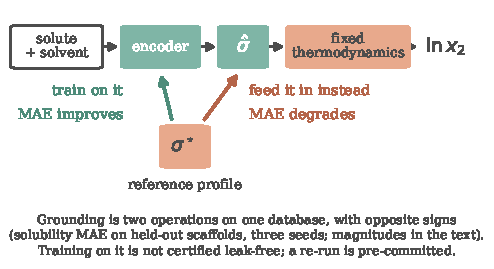
\includegraphics[width=\linewidth]{figs/fig_toc.pdf}
\end{tocentry}

\maketitle
\begin{abstract}
Physics-informed models route a prediction through interpretable physical quantities, on the expectation
that grounding those quantities in accurate reference values improves accuracy. Whether it does depends on
the fixed model that consumes them, and on which sense of grounding is meant. We make that dependence
measurable for solid--liquid solubility: with COSMO-SAC implemented as differentiable
activity-coefficient layers, an external reference for the learned input gives an instrument that splits
the prediction error into a misspecification term and an insufficiency term. The split is an exact
identity; its misspecification bound needs no model fit, but the insufficiency term is estimated by
binning and enters as a one-sided bound. Grounding at \emph{training} time, as supervision from the same
reference database, helps: it improves solubility mean absolute error from $2.04$ to $1.85$ in
$\lnx$ units. Grounding at \emph{inference} time, by substituting the reference profile for the learned
one, hurts: $1.85$ to $2.25$ when the substitution is made at evaluation only, and $1.80$ to $1.98$ at one
seed when the model is allowed to co-adapt to it during training, so about half of the larger figure is
ordinary test-time distribution shift. That substitution falls almost entirely on the solvent channel,
few drug-like solutes carrying a reference profile. On a matched activity axis, where both channels
carry one, the misspecification term of the deployed COSMO-SAC-2002 kernel is likely the larger: on
$477$ infinite-dilution measurements over $185$ molecule pairs it is bounded below by $1.21$ against
an insufficiency term bounded above by $0.70$, a margin of $+0.51$ whose $90\%$ interval spans zero
under two of three clusterings; on the $60$-pair subset for which the paradox's own reference
database is matchable the margin falls to $+0.05$. Both figures are for the combinatorial convention
the pipeline deploys, applied to both sets; the literature-standard convention puts the margins at
$+0.95$ and $+0.58$. Under the modern 2010 kernel the ordering is lost on the small set. Trained end
to end through the misspecified model, the learned profile departs from the reference along a direction
shared across molecules and no longer reports the physical quantity; that this departure cancels part of
the model's error remains unmeasured. The one direct check we can run argues against it but is weak:
it uses a retained checkpoint whose departure is half again the studied one, on the infinite-dilution
rather than the finite-composition axis that produces the drift, and at several times the target
variance, where partial cancellation would be undetectable. Raising the
fixed model's fidelity more than halves its error on the matched corner's hydrogen-bonding chemistry
but does not lower it on representative data. The sign reversal
appears again in a synthetic family of models and, in a second chemical domain---acid dissociation
constants---in at least $19$ of $20$ resampled splits, there through the insufficiency channel rather
than through this mechanism. The instrument applies to any composed predictor: grounded latents are not
reliably interpretable when the model consuming them is misspecified.
\end{abstract}

\section{Introduction}
\label{sec:intro}
The solubility of a solid in a liquid solvent decides how a drug is formulated, how a product is
crystallised and purified, and which synthetic routes are practical, yet it remains hard to predict from
molecular structure alone. Measurements of the same system disagree substantially between laboratories,
and the property depends jointly on how a molecule interacts with the solvent and on the energetics of
its crystalline solid, so first-principles calculation is costly and any data-driven predictor must
generalise to molecules unlike those it was trained on.

Two broad strategies have emerged. Purely data-driven models regress solubility directly from molecular
descriptors or learned representations; they are at present the most accurate on unseen molecules, but
they are opaque and offer no account of why a given prediction succeeds or fails. Physics-informed models
instead route the prediction through interpretable thermodynamic quantities---an activity coefficient
that describes the solute--solvent interaction, and the melting properties of the crystalline solid---each
of which can be calibrated against abundant single-component reference data that a black-box regressor cannot
exploit. The appeal of this second strategy rests on a widely held expectation: that supplying a model
with physical inputs closer to their true values should make its predictions more accurate.

This expectation can fail, and which sense of ``grounding'' is meant decides the sign. We study a
physics-informed solubility model whose learned intermediate is a molecular charge-density profile (a
$\sigma$-profile) consumed by a fixed thermodynamic model, COSMO-SAC. Such a fixed, non-fitted map from a
learned intermediate to a prediction is what we call a \emph{closure}. Supervising the learned profile
against an external quantum-chemical database during training \emph{helps}: it is the difference between
the ungrounded and grounded arms of Table~\ref{tab:si-arms} ($\mathrm{MAE}\ 2.04\to1.85$). Substituting
the reference profile for the learned one at inference \emph{hurts}, and by less than half as much
($1.85\to2.25$ evaluation-only; Fig.~\ref{fig:overview}). Those are opposite operations on the same
database, and only the second is the paradox. The closure is misspecified, and the learned profile,
trained end to end through it, no longer reports the physical quantity it nominally represents; its
departure from the reference has the form a compensation for the closure's error would take, though we do
not measure that the compensation occurs.

Diagnosing such a failure is difficult because the error of a composed predictor confounds two causes:
the closure may be wrong, or the learned inputs may carry too little information. Our central
methodological result is that an external reference for the learned intermediate separates the two
exactly. The identity fits no further model, and neither does the bound it places on the misspecification
term; the insufficiency term is estimated by binning, so the separation is one-sided in either
direction it can fail. On the activity axis it places the accuracy ceiling of the deployed kernel in the
closure rather than in the inputs. Grounding a learned latent on reference values, and reading it as the
physical quantity, is therefore safe only when the model that consumes it is faithful.

\paragraph{Contributions.} This article makes the following contributions.
\begin{enumerate}
\renewcommand{\labelenumi}{(\alph{enumi})}
  \item We implement the COSMO-SAC family of activity-coefficient models as differentiable layers and
  build an instrument that, using an external reference for a model's learned input, splits the
  prediction error into a model-misspecification term and an input-insufficiency term. The bound it
  places on misspecification fits no further model; the insufficiency term is estimated by binning. The
  instrument applies to any predictor that composes a fixed physical model over a learned intermediate.
  \item A graph neural network predicts solubility more accurately from its own learned
  $\sigma$-profiles than from external quantum-chemical reference profiles supplied to the same fixed
  COSMO-SAC closure---predominantly a solvent-channel substitution, few drug-like solutes carrying a
  reference profile. On the activity axis, where solute and solvent alike carry one, the
  misspecification term of the deployed 2002 kernel is the larger on the $n{=}477$ representative set
  and likely so on the $n{=}60$ matched corner; its transfer to the solubility regime is argued, not
  measured.
  \item Raising the closure's fidelity is a lever with a boundary, and we locate it. The standard
  $2002\to2010$ upgrade more than halves the error on the hydrogen-bond-dominated matched corner---so
  there the misspecification term \emph{is} reducible by a better closure---but does not lower it on
  representative data; run block by block within one database and one temperature, the reversal
  tracks the chemistry rather than the profile source or the temperature range. A post-hoc
  correction of the closure's output restores calibration but not accuracy. These are findings about
  \emph{routes out of} the ceiling, not further evidence for where it sits, which is what (b)
  measures.
  \item Trained end to end through the misspecified closure, the learned latent departs from the
  reference along a direction shared across molecules and transferable between them, and so no longer
  reports the physical quantity. Whether that departure \emph{cancels} closure error---which would
  explain why more accurate inputs reduce accuracy---is not established: the only direct check we can
  run on retained checkpoints runs against it, on the wrong axis and with too little power to exclude
  partial cancellation (\S\ref{sec:surrogate}).
  \item The same reversal of the grounding effect appears in a controlled synthetic family of models and
  in a second chemical domain, the prediction of acid dissociation constants, where an in-distribution
  test reproduces both signs of the effect in at least 19 of 20 resampled splits---there through the
  input-insufficiency channel, so it replicates the sign rule and not the mechanism of (d).
\end{enumerate}

The remainder of this article is organised as follows. Section~\ref{sec:related} reviews data-driven and
physics-informed approaches to solubility prediction and the broader question of when imposed physical
structure helps or hurts a learned model. Section~\ref{sec:framework} develops the theory for a composed
predictor and defines the exact separation of model misspecification from input insufficiency.
Section~\ref{sec:methods} describes the model, the data, and the reference-input substitution.
Section~\ref{sec:results} presents the solubility paradox, the measurement that attributes the accuracy
ceiling to the fixed model, the learned latent's departure from its reference, and the synthetic and
second-domain replications. Section~\ref{sec:discussion} discusses the implications and the limitations, and
Section~\ref{sec:conclusion} concludes.

\begin{figure*}[t]
\centering
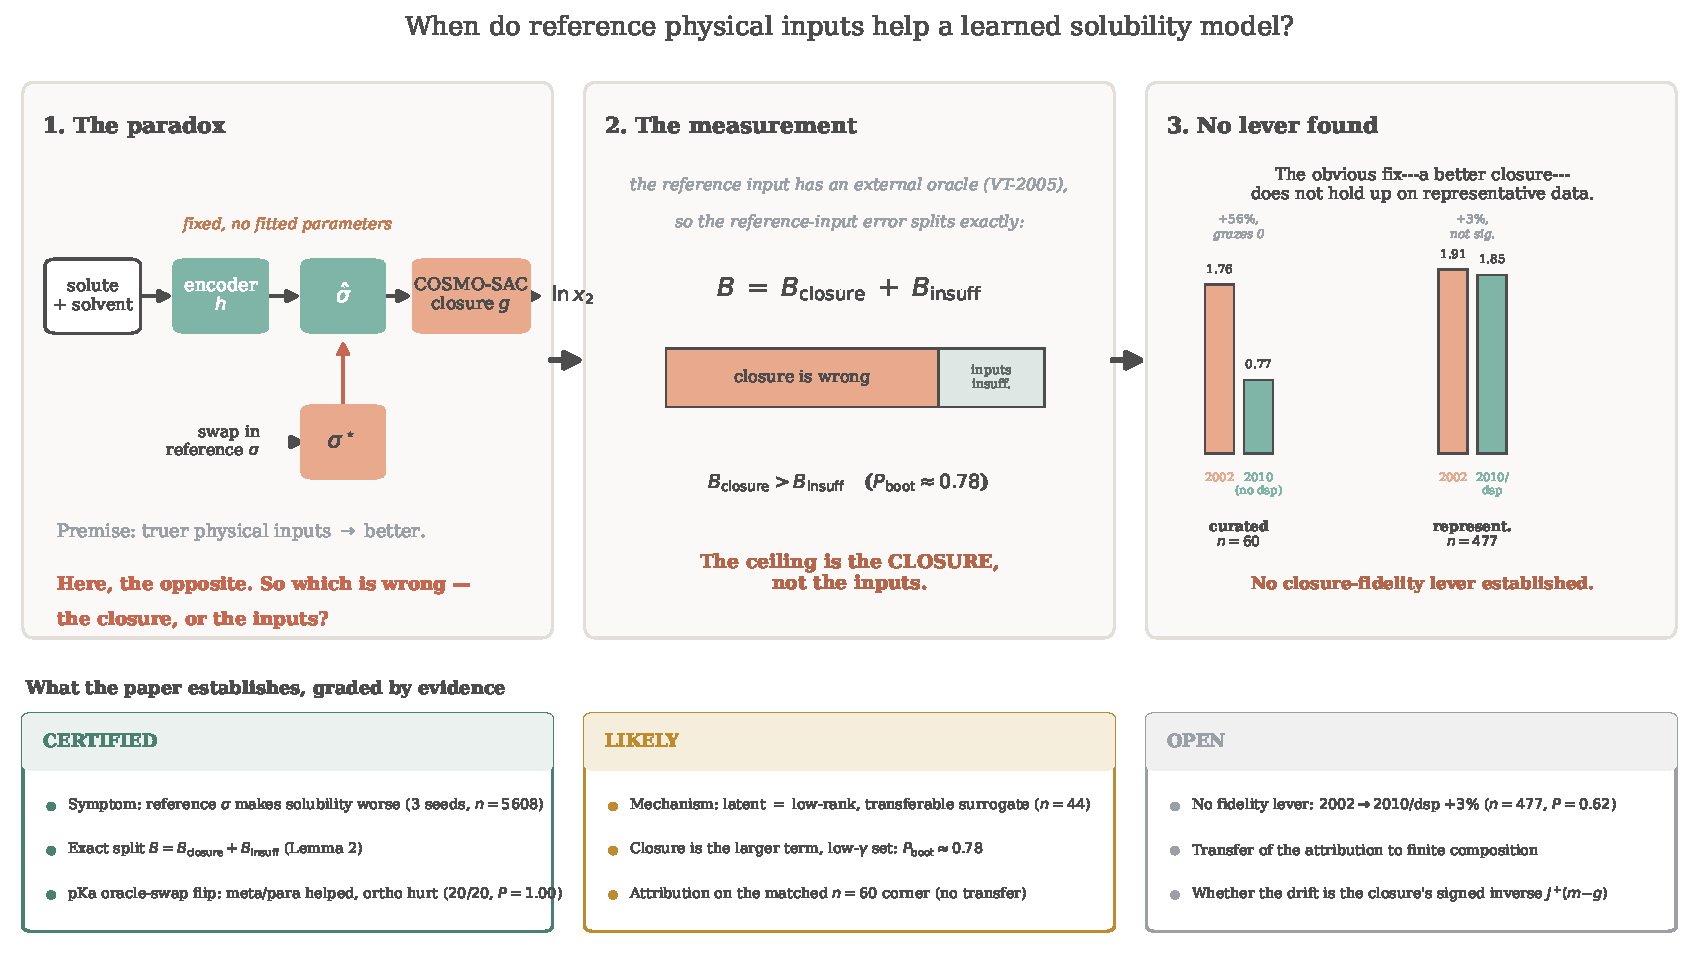
\includegraphics[width=\linewidth]{figs/fig_overview.pdf}
\caption{\textbf{Overview.} \textbf{(a)}~A learned encoder predicts a molecular charge-density
profile $\hat\sigma$, which a fixed thermodynamic model converts into a solubility; substituting an
external quantum-chemical reference profile $\sigma^\star$ for $\hat\sigma$ at evaluation makes the
prediction worse. That substitution is the opposite operation to supervising $\hat\sigma$ against the
same database during training, which helps (\S\ref{sec:paradox}). \textbf{(b)}~The counterpart error
on the activity axis, where solute and solvent alike carry a reference profile, under one-sided
bounds: an upper bound on the input-insufficiency term and the lower bound it implies for the
model-misspecification term, on the representative set ($477$ measurements over $185$ molecule pairs)
under the \emph{deployed} residual-only combinatorial convention, the convention headlined on both
sets (\S\ref{sec:measure}). The two blocks
are contiguous shares of one total, not intervals on an axis; the quantity that orders them is the
separation margin printed in the panel, whose interval spans zero under two of the three clusterings,
so the ordering here is likely rather than resolved. On the $n{=}60$ corner of (a)'s own reference
database it is weaker again, and transfer of either to (a)'s finite-composition regime is argued, not
measured.}
\label{fig:overview}
\end{figure*}

\section{Related work} \label{sec:related}

Two families of methods dominate the prediction of solid solubility and solvation, and they make
opposite choices about physical structure. Physics-informed pipelines such as SolProp
\cite{vermeire2022solprop} assemble a thermodynamic cycle from separately learned components
(solvation free energy, vapour pressure, fusion properties), so that each prediction is decomposable
and its intermediate quantities carry physical meaning. Direct models forgo that structure: FastSolv
\cite{osanloo2024} regresses solubility from molecular descriptors with a deep neural network and is the
current leader on extrapolation to new solutes, a task on which inter-laboratory disagreement sets a
substantial irreducible-error floor. On accuracy the ordering is clear: the black box leads and the
physics-informed cycle trails it.

The activity coefficient is the quantity a solubility model must supply, and learned surrogates for it
have advanced quickly. Winter et al.\ \cite{winter2022} predict infinite-dilution activity coefficients
\lngi\ directly from SMILES with a language model, and Sanchez-Medina et al.\ \cite{sanchezmedina2023}
embed a Gibbs--Helmholtz constraint in a graph network to capture their temperature dependence. These
approaches treat the activity coefficient as the regression target, rather than retaining a mechanistic
model that consumes a predicted molecular property.

The broader question of when a fixed physical structure helps or hurts a learned model is central to
physics-informed machine learning \cite{karniadakis2021}. Its dominant forms impose structure as a
differentiable object: physics-informed neural networks enforce a governing equation through the loss
\cite{raissi2019}, while physics-guided and gray-box hybrids compose learned components with fixed
mechanistic maps \cite{willard2022}, and a recent operator-learning approach adds a trainable correction
to a misspecified governing equation \cite{ma2026}. The prevailing expectation is that more physics
improves generalisation, yet the same structure can degrade it: physics-informed networks have
documented failure modes in which the imposed constraint makes optimisation or accuracy worse
\cite{krishnapriyan2021}. In neural solvers of partial differential equations, Mohan et al.\
\cite{mohan2024} show that a learnable term added to a fixed discretised operator can absorb the
simulation's truncation artifacts rather than the physics, so that the program's apparent
interpretability is illusory; their error source is numerical, and they have no external reference for
the learned term.

The same concern appears in concept-bottleneck models as \emph{concept leakage}, in which a learned
concept silently encodes information beyond its nominal meaning and its interpretation becomes misleading
\cite{mahinpei2021,margeloiu2021,havasi2022}. Recent work traces one route to leakage to the downstream
model rather than to a trainable head: an inflexible or misspecified head forces the encoder to deform
the concept into carrying a dependence the head cannot represent \cite{parisini2025}, and overwriting a
frozen head's leaked concepts with their ground-truth values can then degrade accuracy
\cite{espinosa2025leakage}.

Several diagnostic tools are relevant to such failures. The gap between a fixed physical map and reality
is the model-discrepancy problem of Kennedy and O'Hagan \cite{kennedy2001} and its calibration critique
\cite{brynjarsdottir2014}; separating whether predictions are right on average from whether they are
sharp is the calibration and reliability--resolution decomposition of Murphy and DeGroot
\cite{murphy1973,degroot1983}; and a misspecified model still converges to a well-defined pseudo-true
limit under the quasi-maximum-likelihood account of White \cite{white1982}. That a decomposition may be
only weakly constrained by the data is the subject of parameter sloppiness
\cite{transtrum2015,gutenkunst2007} and of structural versus practical identifiability
\cite{raue2009,villaverde2016}, and the risk that apparent skill reflects pipeline choices rather than
physics is the concern of underspecification \cite{damour2022}, leakage and reproducibility
\cite{kapoor2023}, and compositional risk \cite{mahajan2025crm}.

What this literature lacks is a way to \emph{measure}, rather than merely diagnose, whether a fixed
physical model or its learned inputs limits a composed predictor's accuracy, and to test whether the
learned intermediate has become a surrogate that compensates for the model's error. The concept-leakage
literature identifies the phenomenon but has no external reference against which to quantify it, and the
neural-solver work has a fixed operator but only a numerical, unreferenced error term. We supply the
missing ingredient: an external reference for the learned intermediate---a reference $\sigma$-profile
for solubility, and tabulated substituent constants for a second chemical domain---which turns the
qualitative concern into a model-free measurement that separates model misspecification from input
insufficiency. Using it, we show on a fixed thermodynamic model that the learned intermediate becomes a
low-rank, transferable surrogate, and that grounding it on reference values can therefore reduce
accuracy. Our data are drawn from BigSolDB~2.0 \cite{krasnov2025bigsoldb}; FastSolv and SolProp remain
the accuracy reference points, which we do not contest.


\section{Setup and theory}
\label{sec:framework}
For a solute~$s$ in solvent~$v$ at temperature~$T$, the target is $y=\lnx$, the
log saturated mole fraction. Dissolving a solid trades two costs against each
other---breaking the crystal lattice ($\Phicry$) and mixing the freed molecules
against non-ideal solute--solvent interactions ($\lng$)---and solid--liquid
equilibrium (SLE) sets the log-solubility to their negative sum:
\begin{equation}
  \lnx = -\underbrace{\frac{\dHfus}{\Rgas}\!\Big(\tfrac1T-\tfrac1\Tm\Big)}_{\Phicry(T)\ \text{(crystal)}}
         \;-\;\underbrace{\lng(x_2,T)}_{\text{activity}} ,
  \label{eq:sle}
\end{equation}
with the constant-$\Delta C_p$ (heat-capacity-of-fusion) correction omitted for
clarity. The activity term is produced by a \emph{differentiable closure} $g$:
a graph encoder predicts a $\sigma$-profile---the distribution of screening
(surface) charge density over a molecule, the histogram a COSMO model
consumes---for each molecule, and COSMO-SAC (the COnductor-like Screening
Model--Segment Activity Coefficient \cite{lin2002}, a reformulation of COSMO-RS)
maps the pair of profiles to $\lng$. Write $\zstar$ for the \emph{reference} physical latent, the externally referenced
$\sigma$-profile from the VT-2005 database (the Virginia Tech 2005 compilation of
quantum-chemically computed screening-charge profiles for ${\sim}1{,}400$
compounds \cite{mullins2006}), and $g(\zstar)$ for the closure output when fed the
reference profile. The model's own head instead predicts a \emph{learned} profile
$\hat z$ and evaluates $g(\hat z)$. We call each trained configuration, and each
closure variant we evaluate, an \emph{arm}; a \emph{DirectGNN} control arm shares the
encoder, interaction, readout, capacity and epoch budget but emits $\lnx$ with no
closure, and is the reference against which the cost of the physics bottleneck is
measured (schematic in SI, Fig.~\ref{fig:arch}). Their optimisation settings---dropout,
learning rate, gradient clipping, weight decay---were tuned per arm and differ, so the
gap is not attributable to the bottleneck alone.

\paragraph{The oracle substitution.} Feeding $\zstar$ in place of $\hat z$
(a $\sigma$-oracle) isolates the closure from encoder error: if the closure were
well specified, $g(\zstar)$ should be the best available activity estimate. The
paradox is that it is not.

\paragraph{Data.} Solubility measurements are a Bemis--Murcko scaffold split of
BigSolDB \cite{krasnov2025bigsoldb} (grouping molecules by ring-system-plus-linker
scaffold, side chains stripped), so test solutes share no scaffold with training;
the activity labels $m$ are experimental infinite-dilution activity coefficients
($\lngi$, IDAC) compiled from ThermoML (the NIST/IUPAC archive of experimental
thermophysical data \cite{frenkel2011thermoml}), and the reference $\sigma$-profiles
$\zstar$ are the VT-2005 database.


The results below are stated for a general \emph{composed predictor} $\hat y=g(h(x))$
in which a fixed closure $g$ consumes a learned physical
intermediate $z=h(x)$, and are compared against a matched free predictor that shares the
encoder but drops $g$. Solubility, with $g$ the COSMO-SAC closure and $z$ the
$\sigma$-profile, is one instance; App.~\ref{sec:pka} gives a second (pKa through a fixed
Hammett closure), and App.~\ref{sec:dial} a controlled synthetic family. Nothing in
Lemmas~\ref{prop:ident}--\ref{prop:decomp}, Theorem~\ref{thm:gap}, or
Proposition~\ref{prop:tax} is specific to COSMO-SAC. Two quantities organise the section:
the closure/insufficiency split $B=\Bclos+\Binsuf$, which is the assumption-light
\emph{instrument}, and the observable grounding gap $\Ggap$, which is an \emph{indicator} of
closure misspecification whose validity we characterise.

\subsection{Why a free head can compensate: structural non-identifiability}
The crystal/activity split is not identifiable from solubility data alone, which
is precisely why an unconstrained head can silently absorb crystal error into the
activity term.
\begin{lemma}[Structural non-identifiability of the SLE split]\label{prop:ident}
Consider the infinite-dilution SLE observable $\mu(T)=-\Phicry(T)-\lngi(T)$ with
$\Delta C_p=0$, so that $\Phicry(T)=(\dHfus/\Rgas)(1/T-1/\Tm)$ is affine in $u=1/T$,
and a symmetric two-suffix activity class ($\lng=\lngi\,(1-x_2)^2$) in which
$\lngi(T)$ is affine in $u$. Then, for any design with at least two distinct
temperatures, $\mu$ depends on the parameters only through the two-dimensional
statistic (its slope and intercept in $u$), and the activity intercept and slope
already span that plane;
hence the crystal parameters $(\dHfus,\Tm)$ are unidentified, the profiled Fisher
information for $\dHfus$ is exactly zero, and the indeterminacy set is
two-dimensional. The deficiency is closed only by a rank-completing external
constraint (a direct crystal label, or a fixed activity slope). At finite dilution
the composition factor $(1-x_2)^2$ breaks the exact affinity, leaving a non-zero but
near-degenerate information of order $x_2^2$.
\end{lemma}
\noindent How near-degenerate is a property of the temperature design, not a constant: over
$\Delta T$ from $120$ to $10$\,K the numerical conditioning of the solubility-only design runs from
$1.7\times10^{3}$ to $1.9\times10^{16}$, passing $2.3\times10^{5}$ at the $\Delta T=40$\,K window used
for the audit below (\S\ref{sec:ident}, which states the noise levels, operating point and design that
fix these values).
\noindent This is the standard structural-identifiability picture for a
collinear design \cite{raue2009,villaverde2016}---equivalently the null-space picture of
regularisation theory, in which the component of an inverse fit the data leaves unconstrained
lives in the null space of the forward map and is fixed only by the prior \cite{engl1996,hansen1998},
restated for learned reconstruction as null-space networks \cite{schwab2019}. What is specific to our
setting is that this indeterminate component is not projected out by construction but is left free
under \emph{end-to-end} training of the SLE-coupled latent. We prove it in the SLE form
(App.~\ref{sec:si-proofs}) and audit it numerically in \S\ref{sec:ident}. It is
\emph{enabling background}
rather than a principal claim: it explains why grounding an under-determined factor on
external single-component data is necessary, and why compensation between the
factors is expected. By itself it says nothing about whether grounding helps.
That depends on whether the closure that consumes the grounded inputs is
correctly specified, which is the question we make measurable next.

The non-identifiability is graded by the activity class rather than binary: no information about
$\dHfus$ survives when the activity term can imitate the crystal term's temperature dependence
$\{1,1/T\}$, and some survives once the activity slope is constrained
(Lemma~\ref{prop:semiparam}, App.~\ref{sec:si-proofs}). Restricting that slope leaves
$\mathrm{sd}(\dHfus)\approx8{,}251$\,J/mol---finite but unusable---whereas external crystal labels
close it to $\approx1{,}689$\,J/mol (\S\ref{sec:ident}).

\subsection{The closure--insufficiency decomposition: the instrument}
\label{sec:decomp}
Let $m$ be the activity target (experimental $\lngi$) and $g(\zstar)$ the closure
evaluated on the true latent. The risk of the reference-input path---its mean squared error
$\Ex[(m-g(\zstar))^2]$---decomposes exactly into a part the intermediate cannot resolve (the
irreducible Bayes term) and a part attributable to error in the fixed map; the excess over the Bayes predictor
$\Ex[m\mid\cdot]$ is the second term alone.

\begin{lemma}[Exact closure--insufficiency decomposition and its one-sided bounds]\label{prop:decomp}
For a \emph{fixed} (non-fitted) closure $g$, with $\zstar$ denoting the closure's \emph{entire}
argument (on the representative set of \S\ref{sec:measure} the profile pair together with the
temperature the closure is evaluated at),
\begin{equation}
\begin{aligned}
  \underbrace{\Ex\big[(m-g(\zstar))^2\big]}_{\text{ref.-input MSE}}
  &= \underbrace{\Ex\big[\Var(m\mid \zstar)\big]}_{\Binsuf\ (\text{irreducible})} \\
  &\quad + \underbrace{\Ex\big[(\Ex[m\mid\zstar]-g(\zstar))^2\big]}_{\Bclos\ (\text{decoder bias})} .
\end{aligned}
  \label{eq:decomp}
\end{equation}
The cross term vanishes identically because $\Ex[m\mid\zstar]-g(\zstar)$ is
$\zstar$-measurable and $\Ex[(m-\Ex[m\mid\zstar])\mid\zstar]=0$---which is why $\zstar$ must be the
closure's whole argument and not a part of it. The split is exact with no fitting of the closure
$g$---the cross term vanishes because $g$ is
fixed and $\zstar$ is externally observed---so the total and $\Bclos$'s Jensen lower bound are
fit-free; $\Binsuf=\Ex[\Var(m\mid\zstar)]$, however, must be estimated with a conditional-variance
smoother whose choice affects the verdict (\S\ref{sec:measure}).
\end{lemma}
\noindent Equation~\eqref{eq:decomp} is a bias--variance split of model
discrepancy in the sense of Kennedy--O'Hagan \cite{kennedy2001,brynjarsdottir2014}:
$\Bclos$ is the systematic discrepancy of a fixed physical map, and its dominance over
$\Binsuf$ is the empirical content of the claim that the accuracy ceiling is set by the closure
rather than by the inputs. The split itself is standard; what an externally grounded
$\zstar$ adds is that it can be \emph{measured} rather than assumed. Model-discrepancy
calibration \emph{fits} a correction from held-out observations, whereas here $g$ is fixed and
$\zstar$ externally observed, so the map's error is
\emph{attributed}, not corrected---available only where an external latent oracle exists
(linear free-energy relationships, or LFERs; COSMO and group-contribution closures; thermodynamic
cycles), not in gray-box hybrids. \textbf{Exactness is contingent on $g$ being fixed}: for a \emph{fitted}
decoder the cross term does not vanish and a plug-in point split is invalid (a spurious
$-0.36$ cross term appears when $\Ex[m\mid\zstar]$ is replaced by a fitted estimate). We
therefore report \emph{one-sided bounds}, not a point split (each proved in
App.~\ref{sec:si-proofs}):
\begin{itemize}
  \item $\Bclos \ge (\Ex[m]-\Ex[g])^2$ by Jensen: a constant offset between the
  decoder's mean output and the target is misspecification, not input insufficiency, and
  this bound needs \emph{no smoothness assumption}. Its one requirement is that $m$ and $g$
  share the $\lngi$ reference state, which we check directly (\S\ref{sec:measure}).
  \item $\Binsuf \le \Ex[\Var(m\mid \mathrm{bin}(g(\zstar)))]$, a valid
  \emph{upper} bound (law of total variance, since a binning of $g(\zstar)$
  coarsens $\zstar$).
\end{itemize}
The Jensen constant-offset bound is convention-specific---it separates under the full combinatorial
convention but inverts under the deployed residual-only default---so the separation reported in
\S\ref{sec:measure} rests on the leakage-immune (that is, model-free) law-of-total-variance (LOTV)
bound, and the Jensen numbers are reported in App.~\ref{sec:si-tables}.
Because $\Binsuf=\Ex[\Var(m\mid\zstar)]$ depends only on $(m,\zstar)$, it is
\emph{independent of the combinatorial convention} (full vs.\ residual) at fixed $\zstar$:
disagreement between closures that share one reference profile is decoder disagreement and lands
in $\Bclos$. A kernel that carries its own $\sigma$-averaging, by contrast, changes $\zstar$ itself,
so the 2002-vs-2010 contrast (\S\ref{sec:measure}) is not a fixed-input decoder difference.

\paragraph{What population, what is conditioned on, and what sets the instrument's resolution.}
$\Binsuf$ is only well posed once two things are named: the population over which the conditional
variance is taken, and the variable conditioned on. The first decides whether it can be non-zero at
all; the second decides whether the identity and the bound hold.

The population is the \emph{measurement superpopulation}: a draw is a nominal compound pair
\emph{at a temperature}, together with the conformer, tautomer and protonation state actually
populated under those measurement conditions, and an independent experimental determination of
$\lngi$ for it. The conditioning variable is whatever the closure reads---its full argument. Where
$g$ consumes a temperature as well as a profile pair, as it does on the representative set of
\S\ref{sec:measure}, that argument is $(\zstar,T)$ and every statement below is read against
$\sigma(\zstar,T)$; conditioning on $\zstar$ alone would leave $g$ non-measurable with respect to the
conditioning variable, and then neither the cross term's vanishing nor the coarsening bound would
follow. We write $\zstar$ for the argument throughout and name $T$ explicitly where it enters.
Neither the conformational state nor the replicate determination is part of that argument: $\zstar$
is one fixed, quantum-chemically computed profile per nominal compound. $\Var(m\mid\zstar,T)$ is
therefore the spread of $\lngi$ across the conformational ensemble and across replicate
determinations that share a reference profile and a temperature, and it is non-zero for physical
reasons that have nothing to do with sample size. Experimental label noise $\sigma_\eta^2$ is a
\emph{component} of it, not a term beside it: an independent zero-mean error on $m$ enters
$\Var(m\mid\zstar,T)$ directly, so it is already inside every bound we report and is never added on
(Table~\ref{tab:decomp}). What the deployed design cannot do is \emph{observe} it: VT-2005
assigns one profile per compound, the $44$ matched compounds have distinct profiles (closest pair
$L_2{=}3.4$ against a median profile norm of $44$), and no pair carries a replicate, so on the corner
the design holds no two rows at a common $\zstar$. The representative set comes closer without
reaching it: $359$ of its $477$ rows share a molecule pair with another row, but at a different
temperature, hence at a different $(\zstar,T)$. Every $\Binsuf$ entry of Table~\ref{tab:decomp} is accordingly
an \emph{upper bound} obtained by coarsening, and $\Bclos$ only lower-bounded. Two consequences follow,
and they are what reconcile the bounding apparatus with the injectivity of the design. First the
bounds are conservative in one direction only: if the superpopulation variance were in fact negligible,
the finding would be the stronger $\Bclos=\mathrm{MSE}$, so nothing we report can be an artifact of
having over-estimated $\Binsuf$, and no entry should be read as the share of the error the inputs
contribute. Second, the resampling frequencies quoted below are statements about the
\emph{instrument}, not about the superpopulation: $P_{\mathrm{boot}}$ measures how often the
\emph{measured bound} still falls below $\mathrm{MSE}/2$ under resampling of the clusters, that is,
whether this design resolves the ordering---not the probability that an inequality between two
population quantities holds. A low $P_{\mathrm{boot}}$ is loss of resolution, never evidence for the
inputs. Resolution itself is governed by $\dim(\zstar)/n$, since a conditional variance in
$\dim(\zstar)$ dimensions is a nonparametric problem: on the VT-2005 corner $\zstar$ is a $102$-bin
concatenated profile with $n{=}60$ ($\dim(\zstar)/n\approx1.7$), which is why that set supports bounds
only; on the $n{=}477$ representative set of \S\ref{sec:measure} the ratio is $0.21$ per row and
$0.56$ per distinct molecule pair, and the same bound is far tighter on either count. Where the latent is low-dimensional \emph{and} many-to-one the instrument does
better: the pKa Hammett constant is a \emph{scalar} with $n{=}1004$
($\dim(\zstar)/n\approx10^{-3}$) shared across molecules, so $\Binsuf$ is estimated directly rather
than through a coarsening (App.~\ref{sec:pka})---though that estimator is an out-of-fold regression
residual, hence itself an upper estimate, leaving $\Bclos$ lower-bounded there too.

\subsection{What the instrument resolves, and what it does not}
\label{sec:gap}
The decomposition (\S\ref{sec:decomp}) is the load-bearing measurement---assumption-light, needing
neither a representable encoder nor a lossless bottleneck. Alongside it we report a cheaper, purely
observable quantity: the \emph{grounding gap} $\Ggap:=R_{\mathrm{orc}}-R_{\mathrm{e2e}}$, the
oracle risk minus the best end-to-end risk; the paradox is $\Ggap>0$. Under a representable encoder
(A1) and a lossless bottleneck (A2) it is sandwiched $0\le\Ggap\le\Bclos$, so an observed $\Ggap>0$
would certify $\Bclos>0$ (Theorem~\ref{thm:gap}, App.~\ref{sec:si-proofs}). But A1 is empirically
doubtful (the encoder is transfer-limited: a linear probe drops from train $R^2\approx0.76$ to test
$R^2\approx0.45$) and A2 is unverifiable and physically dubious; when A2 fails, $\Ggap>0$ conflates
closure misspecification with input insufficiency---a well-specified closure with a lossy latent gives
$\Bclos=0$ yet $\Ggap>0$ (App.~\ref{sec:dial}, and the pKa ortho sweep of App.~\ref{sec:pka}). We therefore
read $\Ggap$ as corroborating \emph{evidence} and base the model-dominance conclusion on the
decomposition: \emph{the decomposition is the instrument; $\Ggap$ is the indicator that motivates it}.

\paragraph{When a fixed prior loses; and scope.}\label{sec:tax} The deployed question---does the
\emph{trained} physics model outperform the \emph{trained} black box at sample size $n$?---follows a sign
rule. Writing each trained risk as an asymptote plus estimation variance,
$\Ex[\hat R_{\mathrm{phys}}(n)]\approx R_{\mathrm{e2e}}+V_{\mathrm{phys}}(n)$ and
$\Ex[\hat R_{\mathrm{direct}}(n)]\approx R_{\mathrm{direct},\infty}+V_{\mathrm{direct}}(n)$ with
$V(n)\downarrow0$, the \emph{physics penalty at budget $n$} is
$\mathcal{T}(n)\approx\Delta_\infty+[V_{\mathrm{phys}}(n)-V_{\mathrm{direct}}(n)]$ with
$\Delta_\infty:=R_{\mathrm{e2e}}-R_{\mathrm{direct},\infty}$ its \emph{asymptotic} part. Every
measured arm difference reported below is a value of $\mathcal{T}(n)$ at the budget actually trained,
not of $\Delta_\infty$.
\begin{proposition}[Sign of the physics penalty]\label{prop:tax}
(i)~$\mathcal{T}(n)<0$ (physics helps) iff $V_{\mathrm{direct}}(n)-V_{\mathrm{phys}}(n)>\Delta_\infty$:
the variance a constrained prior saves must exceed its asymptotic bias. (ii)~If
$\Delta_\infty>0$ and the variance gap vanishes ($V_{\mathrm{direct}}-V_{\mathrm{phys}}\to0$),
there is a critical budget $n^\star$ beyond which $\mathcal{T}(n)>0$ for all $n>n^\star$. (iii)~Since
$V_{\mathrm{direct}}-V_{\mathrm{phys}}\le V_{\mathrm{direct}}$, as the black box nears the
aleatoric floor ($V_{\mathrm{direct}}\to0$) the penalty tends to $\Delta_\infty$; this limit is
$\ge0$ when the control is asymptotically Bayes ($R_{\mathrm{direct},\infty}=R_{\mathrm{free}}$, the
risk of an unconstrained predictor), not merely from $V_{\mathrm{direct}}\to0$.
\end{proposition}
\noindent The consequence for grounding is~(ii): a fixed-closure prior with strictly positive asymptotic
bias always loses once the budget passes $n^\star$ (proof in App.~\ref{sec:si-proofs}). There is no
``optimal grounding'' theorem, and the decomposition does not improve out-of-distribution accuracy
(\S\ref{sec:results}). Everything here is measured at infinite dilution, on two sets that differ in
regime: the representative set spans $273$--$403$\,K on the UD profiles and is not a low-$\gamma$
design ($\overline{m}=3.42$), while the VT-2005-matchable corner is $298$\,K and low-$\gamma$
($\overline{m}=0.75$). Transfer of either to the finite-composition
regime in which the paradox is observed is a conjecture (\S\ref{sec:discussion}). We read these
results against existing work on model discrepancy \cite{kennedy2001,brynjarsdottir2014}, parameter sloppiness
\cite{transtrum2015,gutenkunst2007}, identifiability \cite{raue2009,villaverde2016}, misspecification
\cite{white1982}, and underspecification \cite{damour2022}.

% COMPUTATIONAL METHODS.  Since 2026-08-02 this is the whole of Sec. 2: the former "Setup and
% theory" section was folded in here, because the composed predictor, the error split and the
% estimator that measures it are the method, and JCIM does not carry a separate theory section.
% WHAT MAY NOT LEAVE THIS SECTION, however tempting the page saving -- a reader of the main text
% alone must never be able to conclude that a control was not run:
%   * the data, the scaffold split, and what the labels are;
%   * the closure implementation AND its validation, including where the validation stops (the
%     dispersion term), because the fidelity result of Sec. 3.2.3 rests on that boundary;
%   * the evaluation protocol: the three oracle applications, which results are three-seed and which
%     single-seed, and on what row set;
%   * the estimator cell, the convention rule, the stratification rule and the admissibility rule,
%     all four fixed here, before any margin is reported;
%   * every disclosure that qualifies a result -- the separately tuned arms, the scaffold-leak guard
%     being a property of the builder and not of these runs, the wrong-split sigma-stream build, and
%     the placeholder repository.
% Construction detail (the solver's damped map, implicit-function gradients, the three phases by
% name, the loss taxonomy and per-phase weights, the architecture, the NRTL parametrisation, the
% COSMO-SAC constants and the 51-bin grid, all hyperparameters) is in App. A; split hazards, stream
% provenance and the full leak audit in App. F.
\section{Computational methods}
\label{sec:methods}

\subsection{The composed predictor and its error split}
\label{sec:framework}
For a solute~$s$ in solvent~$v$ at temperature~$T$, the target is $y=\lnx$, the
log saturated mole fraction. Dissolving a solid trades two costs against each
other---breaking the crystal lattice ($\Phicry$) and mixing the freed molecules
against non-ideal solute--solvent interactions ($\lng$)---and solid--liquid
equilibrium (SLE) sets the log-solubility to their negative sum:
\begin{equation}
  \lnx = -\underbrace{\frac{\dHfus}{\Rgas}\!\Big(\tfrac1T-\tfrac1\Tm\Big)}_{\Phicry(T)\ \text{(crystal)}}
         \;-\;\underbrace{\lng(x_2,T)}_{\text{activity}} ,
  \label{eq:sle}
\end{equation}
with the constant-$\Delta C_p$ (heat-capacity-of-fusion) correction omitted for clarity. The
activity term is produced by a \emph{differentiable closure} $g$: a graph encoder predicts a
$\sigma$-profile---the distribution of screening (surface) charge density over a molecule,
the histogram a COSMO model consumes---for each molecule, and COSMO-SAC \cite{lin2002}, a
segment-activity reformulation of COSMO-RS, maps the pair of profiles to $\lng$. Inside that
map the segment-interaction energy---the electrostatic-misfit and hydrogen-bonding terms
setting what two surface segments cost each other---is the closure's \emph{kernel}, the part
the published revisions rewrite, so a closure variant is named for the year of its kernel:
the deployed \emph{2002 kernel}, and the \emph{2010 kernel} that types segments as
hydrogen-bond donors or acceptors instead of treating hydrogen bonding with one
parameter. Write $\zstar$ for the \emph{reference} physical latent, the
$\sigma$-profile tabulated in the VT-2005 database \cite{mullins2006}, and $g(\zstar)$ for the
closure output when fed it; the model's own head instead predicts a \emph{learned} profile $\hat z$
and evaluates $g(\hat z)$. Feeding $\zstar$ in place of $\hat z$ (a $\sigma$-oracle) isolates the
closure from encoder error: if the closure were well specified, $g(\zstar)$ should be the best
available activity estimate. Each trained configuration, and each closure variant evaluated, is an
\emph{arm}; a \emph{DirectGNN} control arm drops the closure and emits $\lnx$ directly
(Fig.~\ref{fig:arch}), and the two were tuned separately, so the gap between them is not
attributable to the bottleneck alone (\S\ref{sec:eval}; per-arm settings in
\S\ref{sec:si-methods}).

Everything below is stated for a general \emph{composed predictor} $\hat y=g(h(x))$ in which a
fixed closure $g$ consumes a learned physical intermediate $z=h(x)$, against a matched free
predictor that shares the encoder and drops $g$; solubility is one instance, \S\ref{sec:pka} a
second (pKa through a fixed Hammett closure) and \S\ref{sec:dial} a controlled synthetic family.
Nothing in Lemma~\ref{prop:decomp} or in \S\ref{sec:si-proofs} is specific to COSMO-SAC.

The crystal/activity split of Eq.~\eqref{eq:sle} is not identifiable from solubility alone, which
is why an unconstrained head can silently absorb crystal error into the activity term---an
indeterminate component end-to-end training leaves free rather than projecting out, closed only by
a rank-completing external constraint (Lemma~\ref{prop:ident}, \S\ref{sec:si-proofs}). That is
enabling background: it explains why an under-determined factor needs external single-component
data and why compensation between the factors is expected, and says nothing by itself about
whether grounding helps.

\subsubsection{The closure--insufficiency decomposition}
\label{sec:decomp}
Let $m$ be the activity target---the experimental infinite-dilution activity coefficient
$\lngi$---and $g(\zstar)$ the closure evaluated on the true latent.

\begin{lemma}[Exact closure--insufficiency decomposition and its one-sided bounds]\label{prop:decomp}
For a \emph{fixed} (non-fitted) closure $g$, with $\zstar$ denoting the closure's \emph{entire}
argument (the profile pair together with the temperature wherever the closure reads one),
\begin{equation}
\begin{aligned}
  \underbrace{\Ex\big[(m-g(\zstar))^2\big]}_{\text{ref.-input MSE}}
  &= \underbrace{\Ex\big[\Var(m\mid \zstar)\big]}_{\Binsuf\ (\text{irreducible})} \\
  &\quad + \underbrace{\Ex\big[(\Ex[m\mid\zstar]-g(\zstar))^2\big]}_{\Bclos\ (\text{decoder bias})} .
\end{aligned}
  \label{eq:decomp}
\end{equation}
The cross term vanishes identically, which is why $\zstar$ must be the
closure's whole argument and not a part of it (proof, \S\ref{sec:si-proofs}). The split is exact with no fitting of the closure
$g$, so the total and $\Bclos$'s Jensen lower bound are
fit-free. $\Binsuf=\Ex[\Var(m\mid\zstar)]$, however, must be estimated with a conditional-variance
smoother whose choice affects the verdict (\S\ref{sec:estimator}).
\end{lemma}
\noindent $\Bclos$ is the systematic discrepancy of a fixed physical map in the sense of
Kennedy--O'Hagan \cite{kennedy2001,brynjarsdottir2014}, and its dominance over $\Binsuf$ is the
empirical content of the claim that the accuracy ceiling is set by the closure rather than by the
inputs. Where model-discrepancy calibration \emph{fits} a correction from held-out observations,
here $g$ is fixed and $\zstar$ externally observed, so the map's error is \emph{attributed} rather
than corrected---available only where an external latent oracle exists, not in gray-box hybrids
(\S\ref{sec:si-positioning}). \textbf{Exactness is contingent on $g$ being fixed}: for a
\emph{fitted} decoder the cross term does not vanish and a plug-in point split is invalid, so we
report \emph{one-sided bounds} (proved in \S\ref{sec:si-proofs}):
\begin{itemize}
  \item $\Bclos \ge (\Ex[m]-\Ex[g])^2$ by Jensen: a constant offset between the
  decoder's mean output and the target is misspecification, not input insufficiency, and
  this bound needs \emph{no smoothness assumption}. Its one requirement is that $m$ and $g$
  share the $\lngi$ reference state, which the closure validation of \S\ref{sec:model} establishes.
  \item $\Binsuf \le \Ex[\Var(m\mid \mathrm{bin}(g(\zstar)))]$, a valid
  \emph{upper} bound (law of total variance, since a binning of $g(\zstar)$
  coarsens $\zstar$).
\end{itemize}
Because $\Binsuf$ is bounded above and $\Bclos$ below, a positive \emph{separation margin}
$\mathrm{MSE}-2\Binsuf^{\mathrm{up}}$ establishes that the closure's own error exceeds what input
insufficiency can account for, while a non-positive one is a failure to separate and licenses
nothing: a reversal would need a \emph{lower} bound on $\Binsuf$, which this instrument does not
supply.

\paragraph{What population, what is conditioned on, and what sets the resolution.}
$\Binsuf$ is well posed only once the population and the conditioning variable are named. The
population is the \emph{measurement superpopulation}: a draw is a nominal compound pair \emph{at a
temperature}, together with the conformer, tautomer and protonation state actually populated under
those conditions, and an independent experimental determination of $\lngi$ for it. The conditioning
variable is the closure's full argument, $(\zstar,T)$ where $g$ reads a temperature. Neither the
conformational state nor the replicate determination is part of it, so $\Var(m\mid\zstar,T)$ is the
spread of $\lngi$ across the conformational ensemble and across replicate determinations at one
reference profile and temperature, non-zero for physical reasons unrelated to sample size.
Experimental label noise is a \emph{component} of it, not a term beside it: an independent
zero-mean error on $m$ enters $\Var(m\mid\zstar,T)$ directly, so it is inside every bound we report
and never added on. What the design cannot do is \emph{observe} it, neither set holding two rows at
a common argument (\S\ref{sec:si-repro}), so $\Binsuf$ is reached only from above and $\Bclos$ only
from below. The bounds are conservative in one direction only---were the superpopulation variance
negligible the finding would be the stronger $\Bclos=\mathrm{MSE}$---so nothing reported can be an
artifact of over-estimating $\Binsuf$, and no entry is the share of the error the inputs
contribute. A low $P_{\mathrm{boot}}$, the cluster-bootstrap frequency that the measured margin
stays positive, is likewise loss of resolution and never evidence for the inputs; resolution is
governed by $\dim(\zstar)/n$.

\subsubsection{The decomposition and the grounding gap}
\label{sec:gap}
The decomposition is the measurement the conclusions rest on: assumption-light, needing neither a
representable encoder nor a lossless bottleneck. Alongside it we report a second, purely observable
quantity, the \emph{grounding gap} $\Ggap:=R_{\mathrm{orc}}-R_{\mathrm{e2e}}$, the oracle risk minus
the best end-to-end risk; the paradox is $\Ggap>0$. Under a representable encoder (A1) and a
lossless bottleneck (A2) it is sandwiched $0\le\Ggap\le\Bclos$, so $\Ggap>0$ would certify
$\Bclos>0$ (Theorem~\ref{thm:gap}, \S\ref{sec:si-proofs}). A1 is empirically doubtful---the encoder
is transfer-limited, a linear probe dropping from train $R^2\approx0.76$ to test
$R^2\approx0.45$---and A2 is unverifiable and physically dubious; when A2 fails, $\Ggap>0$ conflates
closure misspecification with input insufficiency, a well-specified closure with a lossy latent
giving $\Bclos=0$ yet $\Ggap>0$ (\S\ref{sec:dial}, and the pKa ortho sweep of \S\ref{sec:pka}). We
therefore read $\Ggap$ as corroborating evidence and base the model-dominance conclusion on the
decomposition.

\paragraph{The sign rule, and scope.}\label{sec:tax} Whether the \emph{trained} physics model
outperforms the \emph{trained} black box at sample size $n$ follows a sign rule with two halves: a
constrained prior helps only where the estimation variance it saves exceeds its asymptotic bias
$\Delta_\infty$, and a prior whose asymptotic bias is strictly positive always loses once the budget
passes a critical size, the variance it saves vanishing as data accumulate while $\Delta_\infty$
does not (Proposition~\ref{prop:tax}, \S\ref{sec:si-proofs}). Each physics-versus-control difference
below is a penalty at the budget actually trained, not an asymptotic one; there is no ``optimal
grounding'' theorem, and the decomposition does not improve out-of-distribution accuracy. Everything
here is measured at infinite dilution on two sets that differ in regime (\S\ref{sec:measure}), and
transfer of either to the finite-composition regime in which the paradox is observed is a conjecture
(\S\ref{sec:discussion}). We read these results against the model-discrepancy, sloppiness,
identifiability, misspecification, underspecification and null-space-prior literatures
(\S\ref{sec:si-positioning}). Spanning two chemical domains, this paper would otherwise use two
letters for more than one quantity each; Table~\ref{tab:notation} gives the renamings that separate
them, and every other symbol is defined where it is used.

% Notation table. Moved from the SI to the main text (2026-07-27) so that the symbols and the coined
% vocabulary are defined before the Results use them, and set at the end of the theory section
% (2026-07-29) when the separate notation-and-grading section was dissolved (criterion 7).
%
% SIMPLIFIED 2026-07-29 under criterion (8). It is a glossary, not a second methods section: one line
% per symbol, the qualification that belongs to a measurement kept where the measurement is made
% (Sec. 5.2, Tables 2-4, App. C). What left this table and where it now stands:
%   - the sets' sizes, temperature and heavy-atom ceiling, and the deposited file names -> Sec. 5.2(i)-(ii)
%   - "label noise is inside B_insuff, not beside it" -> Sec. 3.2 and Table 3, note k
%   - the margin's bootstrap-resolution rule -> the grading rule at the head of Sec. 5
%   - the full inventory of subscripted sigmas (Fisher design, cutoff, derivative) -> App. F, App. G
%   - "deflated" -> App. C, where the deflated estimators are tabulated
% Keep it to one line per row; a row that grows to three is a paragraph in the wrong place.
\begin{table*}[t]
\centering
\caption{Symbols and coined terms used throughout.}
\label{tab:notation}
{\footnotesize
\begin{tabular}{@{}lp{0.68\linewidth}@{}}
\toprule
Symbol / term & Meaning \\
\midrule
$g$ (closure), $h$ (encoder) & fixed, non-fitted physical map (COSMO-SAC; a Hammett linear free-energy relation, LFER, for pKa); learned graph network $x\mapsto z$ \\
$\zstar$, $\hat z$, $m$ & reference (oracle) vs.\ learned $\sigma$-profile; activity target (experimental $\lngi$). $\zstar$ is the closure's whole argument: the concatenated profile pair, written $(\zstar,T)$ where $g$ also reads a temperature \\
$\Bclos$, $\Binsuf$    & closure misspecification $\Ex[(\Ex[m\mid\zstar]-g(\zstar))^2]$; input insufficiency $\Ex[\Var(m\mid\zstar)]$, over the measurement superpopulation of \S\ref{sec:decomp} \\
separation margin      & $\mathrm{MSE}-2\Binsuf^{\mathrm{up}}$; positive witnesses $\Bclos>\Binsuf$ on the sample measured, negative loses that ordering rather than reversing it \\
the corner / the broad IDAC set & the two activity data sets the instrument is run on: the VT-2005-matchable pairs at one temperature, and the larger set matched to the University of Delaware (UD) $\sigma$-profile database across temperatures (\S\ref{sec:measure}) \\
LOTV; leakage-immune & law of total variance, the model-free binning bound on $\Binsuf$; \emph{leakage-immune}, fitting no model, so no held-out row borrows strength from a near-twin \\
\Ggap\ (grounding gap) & $R_{\mathrm{orc}}-R_{\mathrm{e2e}}$: oracle risk minus best end-to-end risk ($R_{\mathrm{free}}$ is the free black box's) \\
$\Gamma_{S}$; \hammett; $\sigma_\eta$ & COSMO-SAC segment activity coefficient (Eq.~\eqref{eq:cosmo}), \emph{not} the grounding gap \Ggap; Hammett substituent constant, renamed from $\sigma$; experimental label noise. Standing alone, $\sigma$ is the charge-density profile, and $\sigma(\cdot)$ with an argument is the generated $\sigma$-algebra \\
$\Delta_\infty$ (physics penalty) & asymptotic risk of the physics arm minus the budget-matched control \\
full / res             & COSMO-SAC with / without the Staverman--Guggenheim combinatorial term \\
compensating surrogate & a learned $\hat z$ that would \emph{cancel} the closure's error instead of matching $\zstar$; the hypothesis of \S\ref{sec:surrogate} \\
$P_{\mathrm{boot}}$    & clustered-bootstrap frequency that the \emph{measured} separation margin stays positive: the instrument's resolution on this design, not a posterior probability \\
\bottomrule
\end{tabular}}
\end{table*}


\subsection{Data, splits, and labels}
\label{sec:data}
Solubility measurements come from BigSolDB~2.0 \cite{krasnov2025bigsoldb}: $127{,}930$ rows over
$15{,}665$ solutes and $221$ solvents between $243$ and $438$\,K, partitioned by Bemis--Murcko
scaffold into $111{,}724$ training, $8{,}103$ validation and $8{,}103$ test rows so that every test
solute is unseen at training; a
melting-point-independent miscibility/structure filter sets row membership, and crystal $\Tm$,
$\dHfus$, Hansen parameters and infinite-dilution activity coefficients \lngi\ are merged on as
per-solute labels where available. Crystal supervision is scarce---the test and validation splits
contain essentially no measured $\dHfus$, the quantitative basis of the identifiability argument
(\S\ref{sec:framework}). The external single-component data used for grounding are an open
crystal-property pool ($\sim$15{,}000 melting points), the VT-2005 $\sigma$-profile database, and
ThermoML infinite-dilution activity coefficients \cite{frenkel2011thermoml}. Two hazards the
pipeline handles explicitly---melting-point unit detection, and the instability of the seeded
scaffold split across pipeline versions---are recorded in \S\ref{sec:si-repro}.

\paragraph{Disclosure: the scaffold guarantee is not certified for these runs.}
The released stream builder excludes any pool molecule whose scaffold appears in validation
or test and aborts on a missing split file --- but that is a property of the builder, not a
certified property of the runs reported here. One $\sigma$-stream build on disk was
generated against the wrong split files, $91$ of its $1425$ rows being held-out solutes by
canonical SMILES, and per-run stream provenance was not logged, so the artifacts cannot certify
which build fed which arm. \S\ref{sec:si-repro} gives the file-order evidence, the three facts that
bound what a leak could do, and the one molecule it touches in the $n{=}44$ analysis of
\S\ref{sec:surrogate}. We therefore do not assert the scaffold guarantee for these runs.

\subsection{Model, closure, and training}
\label{sec:model}
A \emph{shared} message-passing encoder embeds solute and solvent, a bipartite cross-attention block
lets them interact, and the resulting pair representation feeds every head; two interchangeable
encoder alternatives do not outperform it. A fusion head predicts $\Tm$ and $\dHfus$, giving the
ideal term $\Phicry(T)$ of Eq.~\eqref{eq:sle} with the constant-$\Delta C_p$ correction omitted
(audited in \S\ref{sec:si-mech}). The activity term \lng\ comes from one of three differentiable
closures. Two are controls: the fitted NRTL model and its symmetric one-parameter collapse, in which
the identifiability analysis is cleanest (\S\ref{sec:framework}). The third, parameter-free, is the
closure under study---a $\sigma$-profile head emitting a $51$-bin screening-charge-density profile
per molecule, and a COSMO-SAC layer mapping the profile pair to \lng\ with an optional
Staverman--Guggenheim combinatorial term, the full/residual-only distinction on which
Table~\ref{tab:claims} and \S\ref{sec:measure} turn. That closure over a network-\emph{predicted}
$\sigma$-profile, and the intervention that swaps it for the external reference, are the object of
study (\S\ref{sec:paradox}).

The saturated mole fraction solves $\lnx=-\Phicry(T)-\lng(x_2,T)$ as a damped fixed point in $x_2$
(\S\ref{sec:si-methods}); a bounded, gated ``adaptive physics correction'' perturbs the physical
parameters rather than the output, so the physical decomposition survives it. External
single-component data enter through \emph{grounding streams}---the training-time sense of grounding,
a separate operation from the evaluation-time substitution below. Each stream is a sidecar of
\emph{self-solvent} rows ($\mathrm{solvent}=\mathrm{solute}$, no solubility label, only the target
factor's mask active), interleaved into training under the guard above; the streams ground the
crystal factor from the melting-point pool and the activity factor from the $\sigma$-profile
database, identifying from external data a factor that solubility alone leaves non-identifiable
(\S\ref{sec:framework}) and that a black-box predictor cannot use. Training runs a three-stage
curriculum under a weighted loss: a warm-up on the auxiliary streams alone, then joint training
against solubility, then a low-rate stabilisation stage. The schedule pinned for the arms of
Fig.~\ref{fig:paradox} freezes the $\sigma$ head at the end of the warm-up, so the $\sigma$ stream
enters the warm-up only (\S\ref{sec:si-tables}).

\paragraph{The in-house closures, and where their validation stops.}
% Artifact: results/b_insuff/closure_reference_validation.json (2002, rmse 0.0035) via
% scripts/analysis/run_closure_reference_validation.py. The 2010 figure has no deposited
% artifact -- scripts/analysis/validate_cosmo2010_layer.py printed to stdout on the run it
% comes from -- which the SI states.
The dispersion-off closures in the fidelity measurement (\S\ref{sec:fidelity}) are our own
differentiable implementations, so those arms share one code path, and each consumes its own
model-prescribed $\sigma$-averaging (Mullins for 2002, Hsieh for 2010). Our 2002 layer---the
\emph{fair 2002} arm wherever the kernels are compared, because it reads all three profile
channels---reproduces the NIST reference COSMO-SAC-2002~\cite{bell2020cosmosac} to RMSE
$0.0035\,\ln\gamma$ on identical VT-2005 profiles, and our COSMO-SAC-2010/dsp
layer~\cite{hsieh2010,hsieh2014dsp}, built on the \emph{typed} latent of three
donor/acceptor-resolved $\sigma$-profiles per molecule in place of one, reproduces the NIST 2010
reference with dispersion \emph{off}. The dispersion term is \emph{not} validated to that standard,
which is why every dispersion-off contrast is computed on our layers while the \emph{2010,
dispersion on} runs are quoted from \texttt{cCOSMO}. Layer definitions, validation figures and the
full scope of the dispersion caveat are in \S\ref{sec:si-methods}.

\subsection{Evaluation protocol, and the DirectGNN control}
\label{sec:eval}
The \emph{oracle substitution} replaces the predicted $\sigma$-profile $\hat z$ with the reference
VT-2005 profile $\zstar$ before the closure, matched by canonical SMILES. It is applied three ways
to rule out implementation artifacts: at evaluation only; injected at training time so the model
co-adapts; and as a channel-swap control, injected at training under a coordinate-descent schedule
that freezes the crystal branch during the SLE phase, so that only the activity branch refits
against it. The last two are at seed $42$ only. An analogous override substitutes reference crystal
targets. The activity target for the decomposition (\S\ref{sec:measure}) is the infinite-dilution
$\lngi=\lim_{x_2\to0}\lng$, on two sets that differ in their reference database and their regime
(\S\ref{sec:broad}--\S\ref{sec:vt2005}).

DirectGNN shares the encoder, interaction, readout and pair representation, adds a thermometer
(cumulative-threshold) temperature encoding, and maps directly to \lnx\ with no heads, closure or
solver. The two arms therefore share their representation but not their inputs or their tuning: the
control receives an explicit temperature encoding the physics arm does not, seeing $T$ instead
through $\Phi(T)$ and the closure, and the optimisation settings were tuned per arm and differ. The
TGNNSolv$-$DirectGNN gap is accordingly a comparison of two separately tuned pipelines that differ
in the thermodynamic bottleneck, not an isolation of the bottleneck, and every physics-penalty
comparison in \S\ref{sec:results} carries that caveat.

The controlled comparisons of \S\ref{sec:paradox} are run at three seeds and reported as
mean$\pm$sd on a cross-arm row set; $5608$ is that lock, the test rows supervised and finite in
every arm, so all arms score identical rows. Single-seed, and labelled as such where each is
reported, are the training-time and channel-swap oracle controls, the output-residual arms
(\S\ref{sec:gateb}), the data-efficiency curve (\S\ref{sec:data-efficiency}) and the
loss-simplification ablation (\S\ref{sec:si-methods}). The two audit runs behind
\S\ref{sec:measure} are named there with the script and the artifact file of each; not every
artifact those scripts read is small enough to version, and the larger ones are deposited
separately (\S\ref{sec:discussion}).

\subsection{Estimating the split: one cell, one convention, one rule}
\label{sec:estimator}
Four analyst choices set the law-of-total-variance bound---the bin count, where the equal-count bin
edges fall, the within-bin variance convention, and the combinatorial convention---and all four are
fixed here, before any margin is reported.

\emph{The estimator cell.} Eight equal-count bins of $g(\zstar)$, the \emph{unbiased} within-bin
variance, and the row unit, applied identically to every set and every stratum whatever its size.
Enumerating every equal-count contiguous partition, the bin-edge choice is immaterial on the broad
IDAC set and material on the VT-2005-matched set, whose margin changes sign inside the envelope; we
accordingly read that set's $+0.05$ as consistent with zero and carry the claim on the broad set in
stratified form. The binning rule and its envelope are in \S\ref{sec:si-tables}.

\emph{The convention rule.} The margin depends on the combinatorial convention, so one rule governs
both sets: headline the \emph{deployed} residual-only convention, pairing $\mathrm{MSE}$ and the
bound computed under that same convention. Headlining the deployed convention on the smaller set and
the full convention on the broad one would be the favourable choice on each set taken separately;
one rule applied to both costs the broad set's margin about half its value. The Jensen
constant-offset bound is convention-specific---it separates under the full combinatorial convention
and inverts under the deployed residual-only default---so the separation reported in
\S\ref{sec:measure} rests on the model-free law-of-total-variance (LOTV) bound, which fits nothing
and so lets no held-out row borrow strength from a near-twin. $\Binsuf$ is one population quantity
while the two conventions coarsen two different statistics of it, so both bounds are valid on it,
and so is the smaller. The Jensen numbers are in \S\ref{sec:si-tables} and \S\ref{sec:si-proofs}.

\emph{The stratification rule.} The broad set is stratifiable where the VT-2005-matched set's $60$
pairs are not, on two axes that are pure functions of molecular structure: an ordered nine-class
cascade of substructure tests over the solvent, hydrogen-bonding role first and dominant functional
group second, and the solute's role as water or as an organic. The classifier reads a SMILES string
and nothing else---never $m$, $g$, the squared error, the source or the bootstrap---so no cell can
have been chosen on its outcome, which is a property of the code rather than an assurance. A stratum
is \emph{boundable} at $n\ge40$, where eight bins hold five rows; the smaller ones are reported at
that same cell rather than at a rule of their own, with the resample-adaptive rule
$\max(3,\lfloor n/10\rfloor)$ carried beside them in the deposited table, nothing being dropped for
being small.

\emph{The admissibility rule.} A stratum is \emph{admissible} only if it is \emph{(a)}~boundable at
that fixed cell and \emph{(b)}~robust to leave-one-source-out---its margin keeps its sign when each
source publication contributing to it is deleted in turn---in all four
unit\,$\times$\,convention cells, since the map reports all four. That last clause is load-bearing
and is never dropped: without it the set taken whole passes too. A stratum drawing on one publication
fails~(b) by non-testability: there is no deletion to perform, so the sign was never put at risk. A
deletion leaving fewer than $16$ rows leaves the fixed cell undefined and the sign unverifiable,
which fails~(b) as well. Everything else is \emph{reported in the map and not stated}, with its $n$,
its sources, its margin, its interval and the reason. The rule governs the cells that favour us and
those that do not alike, and it tests whether a number is stable and not what it means: an
admissible stratum whose margin is not positive, and an admissible stratum that is another one
restated, both establish nothing.


\section{Notation, and how the claims are graded}
\label{sec:grading}
Table~\ref{tab:notation} fixes the symbols and the coined vocabulary before they are used. Three
collisions are unavoidable in a paper that spans two chemical domains and are resolved by renaming:
$\sigma$ is the charge-density profile throughout, the Hammett substituent constant of
App.~\ref{sec:pka} is written \hammett, and the crystal head's squashing function is written
$\mathrm{logistic}(\cdot)$; the grounding gap is written \Ggap\ so that $\Gamma_{S}$ can keep its
standard COSMO-SAC meaning as the segment activity coefficient of Eq.~\eqref{eq:cosmo}; and label
noise keeps its subscript, $\sigma_\eta$.

% Notation table. Moved from the SI to the main text (2026-07-27) so that the symbols and the coined
% vocabulary are defined before the Results use them, and set at the end of the theory section
% (2026-07-29) when the separate notation-and-grading section was dissolved (criterion 7).
%
% SIMPLIFIED 2026-07-29 under criterion (8). It is a glossary, not a second methods section: one line
% per symbol, the qualification that belongs to a measurement kept where the measurement is made
% (Sec. 5.2, Tables 2-4, App. C). What left this table and where it now stands:
%   - the sets' sizes, temperature and heavy-atom ceiling, and the deposited file names -> Sec. 5.2(i)-(ii)
%   - "label noise is inside B_insuff, not beside it" -> Sec. 3.2 and Table 3, note k
%   - the margin's bootstrap-resolution rule -> the grading rule at the head of Sec. 5
%   - the full inventory of subscripted sigmas (Fisher design, cutoff, derivative) -> App. F, App. G
%   - "deflated" -> App. C, where the deflated estimators are tabulated
% Keep it to one line per row; a row that grows to three is a paragraph in the wrong place.
\begin{table*}[t]
\centering
\caption{Symbols and coined terms used throughout.}
\label{tab:notation}
{\footnotesize
\begin{tabular}{@{}lp{0.68\linewidth}@{}}
\toprule
Symbol / term & Meaning \\
\midrule
$g$ (closure), $h$ (encoder) & fixed, non-fitted physical map (COSMO-SAC; a Hammett linear free-energy relation, LFER, for pKa); learned graph network $x\mapsto z$ \\
$\zstar$, $\hat z$, $m$ & reference (oracle) vs.\ learned $\sigma$-profile; activity target (experimental $\lngi$). $\zstar$ is the closure's whole argument: the concatenated profile pair, written $(\zstar,T)$ where $g$ also reads a temperature \\
$\Bclos$, $\Binsuf$    & closure misspecification $\Ex[(\Ex[m\mid\zstar]-g(\zstar))^2]$; input insufficiency $\Ex[\Var(m\mid\zstar)]$, over the measurement superpopulation of \S\ref{sec:decomp} \\
separation margin      & $\mathrm{MSE}-2\Binsuf^{\mathrm{up}}$; positive witnesses $\Bclos>\Binsuf$ on the sample measured, negative loses that ordering rather than reversing it \\
the corner / the broad IDAC set & the two activity data sets the instrument is run on: the VT-2005-matchable pairs at one temperature, and the larger set matched to the University of Delaware (UD) $\sigma$-profile database across temperatures (\S\ref{sec:measure}) \\
LOTV; leakage-immune & law of total variance, the model-free binning bound on $\Binsuf$; \emph{leakage-immune}, fitting no model, so no held-out row borrows strength from a near-twin \\
\Ggap\ (grounding gap) & $R_{\mathrm{orc}}-R_{\mathrm{e2e}}$: oracle risk minus best end-to-end risk ($R_{\mathrm{free}}$ is the free black box's) \\
$\Gamma_{S}$; \hammett; $\sigma_\eta$ & COSMO-SAC segment activity coefficient (Eq.~\eqref{eq:cosmo}), \emph{not} the grounding gap \Ggap; Hammett substituent constant, renamed from $\sigma$; experimental label noise. Standing alone, $\sigma$ is the charge-density profile, and $\sigma(\cdot)$ with an argument is the generated $\sigma$-algebra \\
$\Delta_\infty$ (physics penalty) & asymptotic risk of the physics arm minus the budget-matched control \\
full / res             & COSMO-SAC with / without the Staverman--Guggenheim combinatorial term \\
compensating surrogate & a learned $\hat z$ that would \emph{cancel} the closure's error instead of matching $\zstar$; the hypothesis of \S\ref{sec:surrogate} \\
$P_{\mathrm{boot}}$    & clustered-bootstrap frequency that the \emph{measured} separation margin stays positive: the instrument's resolution on this design, not a posterior probability \\
\bottomrule
\end{tabular}}
\end{table*}


Each claim below carries a grade where it is stated, and Table~\ref{tab:claims} collects them.
\emph{Certified} means it holds under any closure configuration we evaluate, is exactly proved, or is
bootstrap-certified across resamples of many clusters. \emph{Likely} means measured but sub-threshold,
or one-sidedly bounded, or resolved only on the matched $n{=}60$/$n{=}44$ sets. \emph{Open} means
unestablished, directional, or conjectural. We make no accuracy claim in either direction: the two
arms were tuned separately (\S\ref{sec:methods}), so no difference between them is attributable to the
thermodynamic bottleneck, and every $\Delta\mathrm{MAE}$ in this paper is a difference between
pipelines. Bootstrap frequencies are quoted as bands---rounded to one decimal, with $>0.95$ and
$<0.2$ closing the ends---because with $17$ solvent and $41$ solute clusters on the corner they do not
carry two-decimal resolution (App.~\ref{sec:si-tables}); the two-decimal values are in the deposited
artifacts. The rule is a rounding rule, not a fixed vocabulary, so every frequency in the paper and in
Table~\ref{tab:claims} is quotable within it.

\section{Results}
\label{sec:results}

The instrument (\S\ref{sec:measure}) and the latent's departure from its reference (\S\ref{sec:surrogate})
are the paper's load-bearing contributions: the decomposition locates the ceiling of the deployed
closure in the map rather than in its inputs, and held against its reference on matched pairs the
end-to-end latent no longer reports the physical quantity. The grounding paradox (\S\ref{sec:paradox})
is the observable effect that makes the failure visible but does not by itself carry the attribution;
whether a higher-fidelity closure (COSMO-SAC-2010/dsp) moves the ceiling we could not establish on
representative data (\S\ref{sec:measure}). The synthetic sweep (App.~\ref{sec:dial}), the
output-residual control (\S\ref{sec:gateb}) and the pKa closure (App.~\ref{sec:pka}) stress-test the
account, with further diagnostics in the SI. Table~\ref{tab:claims} states each claim with the set it
is measured on and the grade it carries, and \S\ref{sec:grading} defines those grades before they are
used.

% ---------------------------------------------------------------------------
% Claim ledger: one row per load-bearing claim, so a reader can see data set, n,
% estimator, value and grade without reconstructing them from the prose.
% ---------------------------------------------------------------------------
\begin{table*}[t]
\centering
\caption{What is claimed, where it is measured, and how strongly. ``Margin'' is
$\mathrm{MSE}-2\Binsuf^{\mathrm{up}}$, positive when $\Bclos$ exceeds $\Binsuf$; $P$ is a two-way
(solute\,$\times$\,solvent) cluster-bootstrap frequency, reported as a band (\S\ref{sec:grading}).
LOTV rows use eight equal-count bins, the unbiased within-bin variance, and the \emph{deployed
residual-only} combinatorial convention on both sets---the third analyst choice, named here because
it moves the representative margin from $+0.95$ to $+0.51$ (\S\ref{sec:measure}(i)). Resolution
$\dim(\zstar,T)/n$ is given per row and per distinct molecule pair, since repeated temperatures of
one pair are not independent design points.}
\label{tab:claims}
{\small
\begin{tabular}{@{}p{0.40\linewidth}p{0.17\linewidth}p{0.28\linewidth}l@{}}
\toprule
Claim & Set ($n$) & Value & Grade \\
\midrule
Reference profiles hurt solubility at evaluation (MAE) & test split ($5608$), 3 seeds & $1.85\to2.25$ & certified \\
\ldots and still hurt when injected at training & same lock, seed $42$ & $1.80\to1.98$ & likely \\
Training-time $\sigma$ supervision \emph{helps} (MAE) & same lock, 3 seeds & $2.04\to1.85$ & certified \\
$\Bclos>\Binsuf$, 2002 kernel (LOTV), deployed convention & representative ($477$ rows, $185$ pairs), UD; $\dim/n=0.22$ per row, $0.56$ per pair & margin $+0.51$; $P>0.95$ over pairs, ${\approx}0.9$ two-way and over sources & likely \\
\ldots\ same rows, literature-standard (full) convention & as above & margin $+0.95$, $P>0.95$ (all three clusterings) & likely \\
$\Bclos>\Binsuf$, 2002 kernel (LOTV), deployed convention & corner ($60$), VT-2005; $\dim/n=1.7$ & margin $+0.05$, $P\approx0.7$ & likely \\
$\Bclos>\Binsuf$, 2010 kernel on its \emph{own} typed latent & representative ($477$), UD; $\dim/n=0.64$ per row, $1.66$ per pair & margin $+0.78$, $P\approx0.8$ & likely \\
$\Bclos>\Binsuf$, 2010 kernel on its \emph{own} typed latent & corner ($60$), UD; $\dim/n=5.1$ & margin $-0.61$, $P\approx0.3$ & open (fails) \\
The $2002\to2010$ upgrade lowers the error & representative ($477$) & $-0.07$, $P\approx0.6$ & open (null) \\
\ldots but does on the corner's chemistry, at fixed database and temperature & $57$ pairs shared by both sets, UD & $1.78\to0.77$, $P>0.95$ & likely \\
A fitted kernel residual transfers across solvents & corner ($60$), grouped folds & $-5\pm16\%$ & open (null) \\
The latent departs from its reference along a shared direction & matched molecules ($44$), 3 seeds & $51\pm2\%$ & likely \\
\ldots and the drift's top-two share exceeds a phase-randomised null & one grounded checkpoint, same $44$ molecules & $0.40$ against $0.22\pm0.01$ ($\pm$ is the null's spread) & likely \\
That departure \emph{cancels} closure error & not measured; the direct check is under-powered and runs against it & --- & open \\
Physics arm vs.\ DirectGNN accuracy ($\Delta$MAE) & test split ($5608$), separately tuned arms & $+0.14$ & no claim \\
\bottomrule
\end{tabular}}
\end{table*}


\subsection{The grounding paradox}
\label{sec:paradox}
% Artifacts: results/e5_sigma_grounding/seed_{42,43,44}/comparison.json (3-seed e5 lock, n=5608); aggregate THREE_SEED_SUMMARY.md via run_e5_comparison.py.
% Triple confirmation: eval-oracle / true-at-train / channel-swap.
The word ``grounding'' names two opposite operations on the same VT-2005 database, and they carry
opposite signs. Supervising the $\sigma$ head against the database \emph{during training} improves
solubility MAE from $2.043\pm0.040$ (ungrounded) to $1.846\pm0.053$ (grounded), a larger effect and in
the helpful direction (Table~\ref{tab:si-arms}). Substituting the reference profile for the learned one
\emph{at inference} degrades it, and that substitution alone is the paradox. It fails the way a
\emph{misspecified map} does---not the way missing information would. The effect erases any positive
$R^2$ (Fig.~\ref{fig:paradox}): the model predicts solubility better \emph{from its own learned
$\sigma$-profile} than when \emph{given the external reference one} (MAE $1.85$ vs $2.25$, in $\lnx$
units).

The headline $+0.40$ is the evaluation-only substitution, and it contains a component that has nothing
to do with the closure: any pipeline degrades when an input distribution is swapped at test time. The
control that removes that component injects the reference profile \emph{at training}, so the model
co-adapts; it costs $+0.18$ ($1.80\to1.98$ at seed $42$), so co-adaptation recovers more than half the
headline gap and the confound-free magnitude is the smaller one. A channel-swap control costs $+0.28$.
Both are worse than the learned-$\sigma$ arm, which is what rules out an implementation artifact, but
both are single-seed and fix a sign rather than an effect size.\footnote{The three oracle-application
controls (evaluation-only, training-time injection, channel-swap; \S\ref{sec:methods}) are computed on
the same three-seed cross-arm lock as Table~\ref{tab:si-arms}; only the first is three-seed
(\S\ref{sec:si-tables}). Their per-arm predictions are released with the code.} That the
fault is a wrong \emph{map} rather than a missing input is measured on the activity axis, where the
reference input is clean: restoring the physically \emph{more} complete Staverman--Guggenheim
combinatorial term (the entropic contribution from solute--solvent size and shape mismatch)
\emph{increases} error, and the fixed reference-input closure sits well above the bound on what its
inputs can fail to resolve, under-predicting $\lngi$ with a systematic bias
(SI, Fig.~\ref{fig:parity}).

\paragraph{Why the solubility paradox does not by itself carry the attribution.} The solubility effect is real and
certified (three seeds, three controls), but it cannot carry the closure-versus-input attribution, for a
data reason. Drug-like solutes are essentially absent from the VT-2005 reference set, so the reference
substitution falls almost entirely on the \emph{solvent} channel, and the both-channel substitution the
attribution would need covers only ${\approx}7$ solutes---too few to separate the cause either way.
Computing reference profiles for drug-like solutes costs hundreds of quantum-chemistry runs on large,
multi-conformer molecules, which is not warranted for an effect already certified as a
phenomenon. We therefore carry the causal claim on the activity axis, where the reference
input is clean and matched on both channels: the decomposition (\S\ref{sec:measure}) and the latent's
departure from its reference ($n{=}44$, \S\ref{sec:surrogate}). The title names that axis for this
reason.

\begin{figure*}[t]
\centering
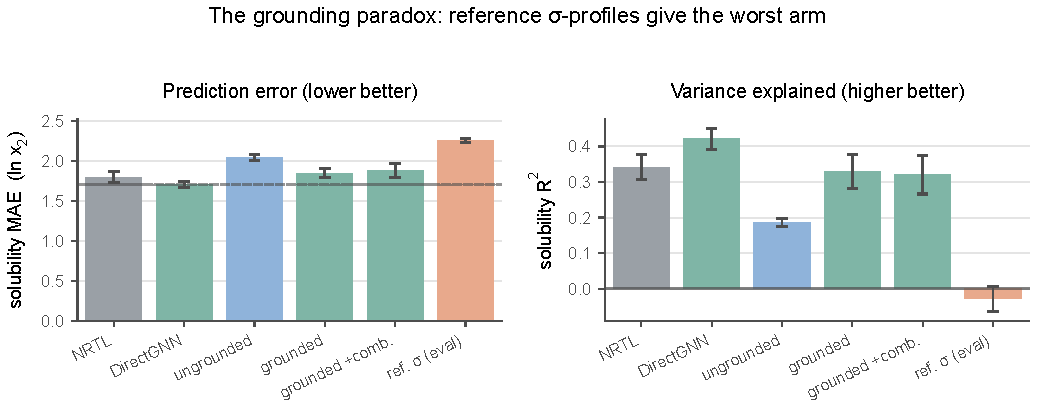
\includegraphics[width=\linewidth]{figs/fig_paradox.pdf}
\caption{Controlled comparison on the scaffold split ($n{=}5608$; solid bars 3 seeds, mean$\pm$sd;
the two hatched bars at the right are the co-adaptation controls and are seed $42$ only, so they
carry no error bar and their $R^2$ was not computed). DirectGNN
shares the encoder but has no thermodynamic model; the physics arms trail it, though the control's
optimisation settings were tuned separately from theirs (\S\ref{sec:framework}). The \emph{NRTL} arm swaps
COSMO-SAC for a more expressive fitted closure (\S\ref{sec:methods}); the four COSMO-SAC arms
differ in how the $\sigma$ head is trained and in what it is fed: \emph{ungrounded} sees no external
$\sigma$ label; the two \emph{grounded} arms add a $\sigma$-profile pretraining stream, the second also
restoring the Staverman--Guggenheim combinatorial term; the \emph{$\sigma$-oracle} (salmon) is the
grounded checkpoint re-evaluated with the external reference VT-2005 profile substituted for the learned
one at test time, where VT-2005 supplies one---in practice almost entirely on the solvent side. That
substitution, not the pretraining stream, is the paradox: it gives the worst arm
($\mathrm{MAE}\ 2.25$ against $1.85$ from the learned profile; $R^2$ to $\approx0$). Because the swap
is made only at evaluation, that bar is annotated in-panel as such: it contains an ordinary test-time
distribution-shift component as well as the closure effect. The co-adapted control that removes that
component---the reference profile injected during training, so the model adapts to it---is the
seventh bar, and costs $+0.18$ against the seed-$42$ learned-$\sigma$ value $1.803$ rather than
$+0.41$; the channel swap is the eighth. The \emph{ungrounded}-to-\emph{grounded} step, in the
opposite direction, is training-time supervision from the same database and \emph{helps}. Per-arm
values are in Table~\ref{tab:si-arms}.}
\label{fig:paradox}
\end{figure*}

\subsection{The closure-fidelity axis: locating the ceiling, and moving it}
\label{sec:measure}
% Artifacts. Corner (n=60): results/b_insuff/decomposition.json via run_b_insuff_decomposition.py;
% bin-count / Bessel / convention grid with per-cell bootstrap: results/b_insuff/estimator_grid.json
% via scripts/analysis/run_b_insuff_estimator_grid.py; blocked-fold and distinct-pair estimators and
% the deployed adaptive-bin bootstrap: results/b_insuff/keystone_robustness.json via
% run_b_insuff_keystone_robustness.py; design composition: results/b_insuff/matched_pairs.csv and
% leverage_robustness.json.
% Representative set (n=477): results/b_insuff/representative_decomposition.json via
% scripts/analysis/run_b_insuff_representative.py (construction ladder, LOTV grid, kernel-contrast
% bootstrap); kernel MSEs cross-checked against results/b_insuff/fidelity_lever_fair2002.json.
% Round-2 design/provenance audit: results/b_insuff/representative_audit.json via
% scripts/analysis/run_b_insuff_representative_audit.py -- distinct-pair counts, pair-blocked
% out-of-fold estimators, within-pair variance across T, collapse to 185 design points, method and
% source-DOI composition, GC-only margin, DOI- and pair-clustered bootstraps, the 2002-vs-2010
% contrast split into the shared 57 and complementary 420 rows, the corner LOTV bound recomputed
% with z* = the UD profile pair (so the corner floor check is same-database), and both sets' floors
% under the 2010 kernel's own typed latent.
The externally-referenced decomposition of \S\ref{sec:decomp} acts as an \emph{instrument}: it asks
whether a fixed closure's ceiling sits in the map or in its inputs. This subsection runs it on two
data sets that must not be conflated---\emph{(i)}~the \emph{representative set}, $n{=}477$
infinite-dilution activity pairs at all temperatures on the University of Delaware (UD) profiles the
deployed COSMO-SAC-2002 kernel consumes there, and \emph{(ii)}~the \emph{corner}, the $n{=}60$ pairs
at $298$\,K for which the paradox's own reference database, VT-2005, supplies both profiles---and then
turns \emph{(iii)} to whether a better closure moves the ceiling. A better-resolved counterpart in
another domain is the scalar-latent pKa closure (App.~\ref{sec:pka}), where the same instrument
recovers the a-priori channel assignment (there, insufficiency)---evidence the instrument works, not
a re-confirmation of this verdict.

\paragraph{(i) The decomposition on the representative set ($n{=}477$).} The closure reads a
temperature as well as a profile pair, and is evaluated here at each row's own temperature, so the
conditioning variable is the closure's full argument $(\zstar,T)$---the concatenated UD
solute/solvent profile pair together with $T$, $103$ dimensions against $n{=}477$
($\dim/n\approx0.21$). Both the identity of Lemma~\ref{prop:decomp} and the LOTV bound are read
against \emph{that} $\sigma$-field, under which $\mathrm{bin}(g(\zstar,T))$ is a coarsening and the
cross term vanishes; conditioning on the profile pair alone would license neither, since $g$ is then
not measurable with respect to the conditioning variable. The target $m$ is the experimental $\lngi$,
so floor and closure error are measured on one data set and one profile database. Construction in
\S\ref{sec:si-repro}: $78$ solutes, $36$ solvents, $35$ temperatures from $273$ to $403$\,K, and
$185$ \emph{distinct} solute--solvent pairs---$118$ of them carrying a single row, the largest $15$,
median one. Counted in rows the set is eight times better resolved than the corner; counted in
distinct pairs, three times ($103/185\approx0.56$ against $102/60\approx1.7$). We give both, the
second being the conservative count.

One asymmetry in the matching deserves naming, because it runs against the ordering we claim. The
corner is matched to VT-2005 by canonical SMILES, a rule we defend there on the ground that a profile
imported across a tautomer or protonation variant is the wrong $\zstar$; the representative set is
matched to UD by InChIKey with a first-block fallback, which is looser, and a wrong $\zstar$ inflates
$\mathrm{MSE}$ and so $\Bclos$. The exposure is small and we measure it rather than argue it: of the
$90$ distinct molecules here, $86$ resolve by full InChIKey and four only through the first block,
touching $12$ of the $477$ rows. On the $465$ rows matched exactly the verdict is unchanged---deployed
convention $\mathrm{MSE}\ 1.930$, $\Binsuf\lesssim0.70$, margin $+0.53$ at $P\approx0.9$; full
convention $1.926$, $0.49$, $+0.94$ at $P>0.95$---so the looser rule is not carrying the result.

\emph{One convention rule, applied to both sets.} The margin depends on the combinatorial convention,
so we fix the rule before the numbers: headline the \emph{deployed} residual-only convention, pairing
$\mathrm{MSE}$ and the LOTV bound computed under that same convention, on the representative set and
on the corner alike. An earlier draft headlined the deployed convention on the corner and the full
convention here, which is the favourable choice on each set taken separately; that inconsistency is
removed, and it costs the representative margin about half its value.

Under that rule the deployed 2002 kernel scores $\mathrm{MSE}=1.902$ against $\Var(m)=4.85$, the
LOTV bound gives $\Binsuf\lesssim0.70$ and hence $\Bclos\gtrsim1.21$, at eight equal-count bins under
the \emph{unbiased} within-bin variance: a separation margin of $\mathbf{+0.51}$. The full convention
on the same rows gives $1.911$ against $\Binsuf\lesssim0.48$, margin $+0.95$, and is reported
throughout as the comparison rather than the headline. The margin is positive in all $56$ cells of a
bin-count ($3$ to $48$) $\times$ variance $\times$ convention grid; within the deployed convention its
smallest values are $+0.01$ at four bins and $+0.10$ at three, where the bound is valid but weakest,
and it exceeds $+0.48$ at every bin count from five upward. Three clusterings of the bootstrap
disagree in resolution, and we report all three rather than the most favourable: over the $185$
molecule pairs $P>0.95$ ($90\%$ margin $[+0.23,+1.16]$); two-way over the $78\times36$
solute/solvent clusters $P\approx0.9$ ($[-0.08,+2.16]$); over the $15$ source publications
$P\approx0.9$ ($[-0.07,+1.74]$). Two of the three intervals graze zero, so on the deployed convention
the representative ordering is \emph{likely}, not resolved---the grade Table~\ref{tab:claims} carries
for it. Under the full convention all three clear ($P>0.95$; $[+0.71,+1.27]$, $[+0.48,+1.85]$,
$[+0.50,+1.57]$). Collapsing to one row per distinct pair---$185$ design points, each the row nearest
$298$\,K---gives $\mathrm{MSE}=1.540$, $\Binsuf\lesssim0.63$ and a margin of $+0.27$ at $P\approx0.8$
on the deployed convention ($1.679$, $0.49$, $+0.69$, $P>0.95$ on the full one), so the verdict is
not an artifact of counting repeated measurements of one pair as independent draws, but it is not
sharpened by removing them either.

\emph{The tighter of the two bounds is admissible, and we do not headline it.} $\Binsuf$ is the same
population quantity under both conventions (\S\ref{sec:decomp}); what differs is the statistic the
coarsening bins on, $g_{\text{full}}(\zstar,T)$ or $g_{\text{res}}(\zstar,T)$, each a deterministic
function of the same argument and each therefore giving a separately valid upper bound. The smaller
of the two is consequently also a valid upper bound in population, and charging it against the
deployed error gives $1.902$ against $2\times0.48$, a margin of $+0.94$ (on the corner, $1.472$
against $2\times0.61$, $+0.26$). We report this but do not headline it: a minimum over two
finite-sample estimates is anti-conservative even when each is valid in population, and the
same-convention pairing is the conservative reading.

Two disclosures qualify the corroborating estimators, not the bound. First, the out-of-fold values we
previously quoted were leaked in exactly the way we had disqualified them for on the corner: under
random folds a held-out row's own molecule pair sits in the training fold at a neighbouring
temperature. Blocking folds on the pair moves the random forest from $0.15$ to $0.88$ and the ridge
from $0.80$ to $1.47$, and only the first still clears the $\mathrm{MSE}/2=0.96$ threshold. The LOTV
bound is untouched, having no fold design to leak through---which is why it, and not the agreement of
three estimators, carries the verdict. Second, molecule-pair identity is itself a coarsening of
$(\zstar,T)$, so $\Ex[\Var(m\mid\text{pair})]$ is by the same law-of-total-variance argument a valid
upper bound on $\Binsuf$---over the subpopulation that supports it, the $359$ rows sharing a pair
with another. It is $0.046$, thirteen times tighter than the binning bound on those same rows
($0.61$), and it would put the margin there at $+2.16$ rather than $+0.51$. We do not promote it,
for a reason that is itself informative: all $67$ multi-row pairs draw their rows from a
\emph{single} publication, so within-pair rows are one laboratory's temperature series and not the
independent determinations the superpopulation of \S\ref{sec:decomp} draws. That bound therefore
measures the conformational and within-series components of $\Var(m\mid\zstar,T)$ and not the
between-laboratory one, which is exactly the component the binning bound does sample, its eight bins
mixing all $15$ sources. Read together the two say the binning bound is slack rather than that
$\Binsuf$ is negligible; and the same fact---that the temperature axis carries under $1\%$ of
$\Var(m)$ at a fixed profile pair---makes the choice between conditioning on $\zstar$ and on
$(\zstar,T)$ numerically immaterial here, though only the latter is licensed and it is the one we use.

The labels are also stratifiable, which the corner's $60$ pairs were not: $334$ rows chromatographic,
$37$ chemical or heterogeneous equilibration, $106$ carrying no method field, over $15$ publications
in four journals of which the largest contributes $105$ rows. Restricting to the chromatographic
rows---the cut that \emph{inverted} the enlarged $298$\,K corner of Limitation~(i)---does not invert
here under either convention, but it does not uniformly widen the margin either: on the deployed
convention it narrows it from $+0.51$ to $+0.31$ ($\mathrm{MSE}\ 1.474$ against
$\Binsuf\lesssim0.58$, $P\approx0.9$), on the full convention it widens it from $+0.95$ to $+1.06$
($1.783$ against $0.36$, $P>0.95$). What matters is that neither reproduces the corner's sign change.
On the set the deployed kernel is actually used on, the ceiling is in the map.

\paragraph{(ii) The decomposition on the corner ($n{=}60$).} The corner is where the paper's other
reference-matched analyses live, and it is far weaker: all $60$ rows sit at $298$\,K, so $\zstar$ is
the profile pair alone and $\dim(\zstar)/n\approx102/60$ leaves the split behind one-sided bounds. It
spans $41$ solutes and $17$ solvents (two formamide pairs excluded for a canonical-SMILES tautomer
mismatch), and it is strongly unbalanced: methanol occupies $25$ of the $60$ rows ($12$ as solute,
$13$ as solvent), pyridine is the largest solvent stratum ($20$ rows), and the two worst-fit
pairs---$1$-hexanamine and cyclohexylamine in methanol---carry $34\%$ of the squared error. Both rest
on a single record, and the first sits far off its own homologous series ($\lngi{=}2.62$ against
$-0.78$ for $1$-butanamine in the same solvent), so we do not read that concentration as established
chemistry; the separation survives their deletion ($\mathrm{MSE}\ 1.01$, $\Binsuf^{\text{up}}\ 0.44$).
These are not $60$ exchangeable observations, and the folds below hinge on the same molecules. Of the
$60$ pairs, $57$ also appear in the representative set at $298$\,K under UD profiles, so the two are
not independent samples---the corner is the sub-design on which VT-2005, and therefore the paradox's
own oracle, is defined.

\begin{table*}[t]
\centering
\caption{Closure--insufficiency decomposition on the reference-input activity path, reported as bounds
rather than a point split, under the ``full'' (with Staverman--Guggenheim combinatorial term) and
``res'' (residual-only) conventions, on the representative set ($n{=}477$, UD profiles) and on the
corner ($n{=}60$, VT-2005 profiles). \textbf{The headline columns are the deployed residual-only ones
on \emph{both} sets}, one rule applied throughout (\S\ref{sec:measure}(i)); the full-convention
columns are the comparison. The input-insufficiency ($\Binsuf$) rows are upper bounds; the
load-bearing row is the law-of-total-variance (LOTV) bound on the model-misspecification term
$\Bclos$, which fits no model to the data. The headline LOTV rows use the unbiased
(Bessel-corrected) within-bin variance at eight equal-count bins of $g(\zstar,T)$; the
maximum-likelihood variance, which is biased in the favourable direction, is given beneath for
comparison. The separation margin $\mathrm{MSE}-2\Binsuf^{\mathrm{up}}$ is the quantity that orders the
two terms; its full bin-count $\times$ variance $\times$ convention grid, with a bootstrap frequency
per cell, is Table~\ref{tab:grid} for the corner and Table~\ref{tab:grid-rep} for the representative
set. Because $\Binsuf$ is one population quantity while the two conventions coarsen two different
statistics of the same argument, the \emph{smaller} of the two LOTV bounds is also a valid upper
bound; that reading is given as its own row and is not headlined
(\S\ref{sec:measure}(i)). The corner columns are VT-2005 throughout; the \emph{same} $60$
molecule pairs scored on UD profiles---the database the kernel-fidelity comparison runs on---give
$\mathrm{MSE}\ 1.757$ against a UD-native $\Binsuf\lesssim0.54$, margin $+0.69$, and the two corner
MSEs differ in nothing but the profile database (\S\ref{sec:measure}(iii)). On the representative set
the conditioning variable is the closure's whole argument $(\zstar,T)$. \emph{Deflated}: biased low
by the crossed design, in which two pairs sharing a molecule agree on $51$ of the $102$ $\zstar$
coordinates.}
\label{tab:decomp}
{\small
\begin{tabular}{@{}p{0.44\linewidth}rrrr@{}}
\toprule
 & \multicolumn{2}{c}{representative ($477$)} & \multicolumn{2}{c}{corner ($60$)} \\
\cmidrule(lr){2-3}\cmidrule(lr){4-5}
Quantity & \textbf{res} & full & \textbf{res} & full \\
\midrule
MSE$_{\text{total}}=\Bclos+\Binsuf$ (exact)      & $1.90$ & $1.91$ & $1.47$ & $1.80$ \\
$\Binsuf$ upper (LOTV, $8$ bins, unbiased variance) & $0.70$ & $0.48$ & $0.71$ & $0.61$ \\
$\Bclos$ lower $=\mathrm{MSE}-\Binsuf^{\text{up}}$ (\emph{load-bearing}) & $1.21$ & $1.43$ & $0.76$ & $1.19$ \\
\quad separation margin $\mathrm{MSE}-2\Binsuf^{\text{up}}$ & $\mathbf{+0.51}$ & $+0.95$ & $\mathbf{+0.05}$ & $+0.58$ \\
\quad \dots\ bootstrap band, pair / two-way / source clusters & $>\!0.95/{\approx}0.9/{\approx}0.9$ & $>\!0.95$ (all three) & \multicolumn{2}{c}{${\approx}0.7$ / ${\approx}0.9$ (two-way; no source clusters)} \\
\quad same rows, maximum-likelihood within-bin variance ($\Binsuf$ upper / margin) & $0.69/{+}0.53$ & $0.47/{+}0.96$ & $0.62/{+}0.24$ & $0.53/{+}0.74$ \\
\quad tighter of the two conventions' bounds, charged against the deployed MSE (not headlined) & \multicolumn{2}{c}{$0.48$, margin $+0.94$} & \multicolumn{2}{c}{$0.61$, margin $+0.26$} \\
$\Binsuf$ upper (RF / ridge out-of-fold, random folds --- \emph{leaky}) & \multicolumn{2}{c}{$0.15/0.80$} & \multicolumn{2}{c}{$0.56/0.62$} \\
\quad same, folds blocked on the molecule pair (corner: on both molecules) & \multicolumn{2}{c}{$0.88/1.47$} & \multicolumn{2}{c}{$3.65$/div.} \\
$\Ex[\Var(m\mid\text{pair})]$, binning-free, on the $359$ rows that support it (single-source; \S\ref{sec:measure}(i)) & \multicolumn{2}{c}{$0.046$} & \multicolumn{2}{c}{--- (no repeated pairs)} \\
$\Binsuf$ (k\textsc{nn}-in-$\zstar$, convention-indep., deflated / least conservative) & --- & --- & $0.40$ & $0.40$ \\
label noise $\sigma_\eta^2$ (IDAC) & \multicolumn{4}{c}{a \emph{component} of $\Binsuf$, not a term beside it: already inside every row above (\S\ref{sec:decomp})} \\
\bottomrule
\end{tabular}
}
\end{table*}

\begin{figure*}[t]
\centering
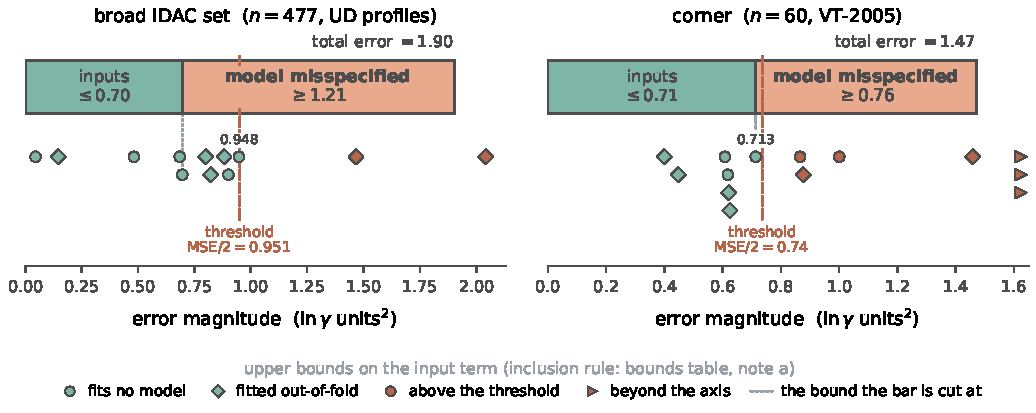
\includegraphics[width=\linewidth]{figs/fig_decomposition.pdf}
\caption{One-sided bounds on the closure--insufficiency split, both panels under the \emph{same}
deployed residual-only convention. \emph{Left:} the representative set ($n{=}477$, UD profiles).
\emph{Right:} the corner ($n{=}60$, VT-2005). Each bar is the total error, cut at the headline LOTV
upper bound on input insufficiency (teal, eight equal-count bins under the \emph{unbiased} within-bin
variance); the remainder is the lower bound this implies for model misspecification (salmon, as in
Fig.~\ref{fig:overview}(b)). The segments are contiguous---they sum to the MSE---so the separation is
the margin $\mathrm{MSE}-2\Binsuf^{\text{up}}$ printed in each panel, not a gap on the axis; the dashed
line is the separation threshold $\mathrm{MSE}/2$, which every plotted $\Binsuf$ bound must fall below
for the ordering to hold. The inclusion rule is now the same in both panels: every $\Binsuf$ upper
bound reported anywhere in the paper for that set is plotted, and any that exceeds the panel's range
is drawn at the right edge as an arrow and labelled \emph{off scale}. That is what the corner's
molecule-blocked estimators are---random forest $3.65$ and $k$NN $1.83$, both above the total MSE and
therefore vacuous, with $k$NN $1.46$ on scale and ridge divergent---and an earlier version of this
figure omitted them while claiming completeness. Also drawn: on both sets the maximum-likelihood
variant of the headline bound and the bound obtained under the \emph{other} combinatorial convention,
which is separately valid (\S\ref{sec:measure}(i)); on the corner the deliberately aggressive
out-of-fold ridge ($0.88$) and the two $\zstar$-conditioning smoothers flagged \emph{deflated}; on the
representative set both the random-fold out-of-fold values, which leak through a held-out row's own
molecule pair at a neighbouring temperature, and the \emph{pair-blocked} ones that do not---blocking
costs the random forest its tightness ($0.15\to0.88$) and pushes the ridge across the threshold
($0.80\to1.47$, in the threat colour)---together with the binning-free
$\Ex[\Var(m\mid\text{pair})]=0.046$, which is valid on the $359$ rows supporting it but samples no
between-laboratory spread. The binning bound, which fits nothing, is unaffected by any fold design.
The headline margin is $+0.51$ on the representative set and $+0.05$ on the corner.}
\label{fig:decomp}
\end{figure*}

\paragraph{The separation margin, and the choices it depends on.} Since the two terms sum to the total,
$\Bclos>\Binsuf$ follows whenever $\mathrm{MSE}$ exceeds the \emph{separation threshold}
$2\Binsuf^{\text{up}}$; the excess $\mathrm{MSE}-2\Binsuf^{\text{up}}$ is the \emph{separation margin}.
The threshold uses an upper bound, so a negative margin loses the separation rather than reversing it.
On the corner under the deployed residual-only convention and the \emph{unbiased} within-bin variance,
the LOTV bound gives $\Binsuf\lesssim0.71$ and $\Bclos\gtrsim0.76$---that is, $1.47$ against a threshold
of $1.42$, a margin of $\mathbf{+0.05}$. We headline that number rather than the maximum-likelihood
variant, which biases the within-bin variance downward and so the margin upward ($\Binsuf\lesssim0.62$,
margin $+0.24$); on the corner the honest statement is that the ordering holds by a margin the design
cannot resolve. Three analyst choices set it---bin count, variance convention, combinatorial
convention---and Table~\ref{tab:grid} gives all $72$ cells with a per-cell bootstrap frequency. The
margin is positive in $66$ of them and non-positive only at the coarsest conditioning, three bins in
either convention and four bins residual-only, where the bound is valid but weakest; and, as
\S\ref{sec:si-tables} sets out, finer bins buy their sharpness with a finite-sample downward bias in
the within-bin variance, so no cell in that grid is unambiguously the right one.

The bound fits no model to the data, which is all \emph{leakage-immune} means here, not that it is
unbiased. The out-of-fold estimators do not control the remaining bias independently, on either set.
On the corner, under random folds every held-out row shares its solvent ($78\%$ of rows) or its solute
($42\%$) with a training row, and two pairs sharing a molecule agree on $51$ of the $102$ $\zstar$
coordinates exactly; blocking folds on both molecules then leaves nothing informative (RF $3.65$,
above $\Var(m){=}2.47$; ridge divergent; $k$-NN $1.83$ and $1.46$), three of them exceeding the total
MSE $1.47$, beyond which an upper bound on $\Binsuf$ constrains $\Bclos$ vacuously. On the
representative set the leak is the near-twin row at a neighbouring temperature, with the cost given in
paragraph~(i). Either way they blunt the instrument rather than refute the separation, and none
supports it either: what eight times the data buys is a sharper \emph{binning} bound, not a working
out-of-fold one.

% Fold and leverage stress-tests: results/b_insuff/keystone_robustness.json and
% results/b_insuff/leverage_robustness.json via scripts/analysis/run_b_insuff_keystone_robustness.py
% and scripts/analysis/run_b_insuff_leverage.py.
% The both-roles methanol deletion (n=35) is in neither file; it is recomputed from
% results/b_insuff/matched_pairs.csv with lotv_binning() of run_b_insuff_decomposition.py
% (res convention): margin MSE-2*B_insuff = 0.346 -> 0.106 at 6 bins, 0.236 -> 0.003 at 8.
On the corner the separation is stable but \emph{not resolved}. It survives all $17$ leave-one-solvent
and all $60$ leave-one-pair folds and deletion of the eight highest-error pairs, but only $40$ of $41$
leave-one-solute folds (six equal-count bins): the exception drops methanol, the maximum-leverage
solute ($12$ pairs), and loses the separation ($-0.26$), as does dropping methanol as solute with
pyridine as solvent ($n{=}28$; $-0.36$). Deleting methanol from both roles ($n{=}35$) holds only
marginally---the margin falls from $0.35$ to $0.11$ at six bins and from $0.24$ to $0.003$ at eight,
and inverts under the Bessel-corrected variance ($-0.03$, $-0.21$). Those fold counts and the
bootstraps use the maximum-likelihood variance. A two-way cluster bootstrap places the margin above
zero in ${\approx}0.8$ of resamples under that variance and ${\approx}0.7$ under the unbiased one
($90\%$ margin spanning zero), and a deliberately aggressive out-of-fold ridge loses the ordering
($\Binsuf\lesssim0.88$ against $\Bclos\gtrsim0.59$). On the corner, then, ``the larger'' is
estimator-conditional and likely rather than certain, and with $17$/$41$ clusters the band is coarse.
The representative set, with $78$/$36$ clusters and a margin an order of magnitude larger relative to
its spread, carries the verdict; the corner shows it is not overturned where VT-2005 and hence the
paradox's own oracle live. Experimental label noise needs no separate accounting: under the population
of \S\ref{sec:decomp} it is a component of $\Binsuf$, already inside every bound reported, and what we
cannot do is subtract it out. Its arithmetic is favourable in any case---zero-mean noise raises
$\mathrm{MSE}$ and $\Binsuf^{\text{up}}$ alike, leaving the $\Bclos$ bound unchanged and shrinking the
margin by $\sigma_\eta^2$---so noise can understate the separation but not create it. The margin
instead bounds a label systematic tracking $\zstar$, which enters $\Bclos$ and closes the separation at
root-mean-square $0.49\,\ln\gamma$ on the maximum-likelihood binning but only ${\approx}0.21$ on the
Bessel-corrected one. The matched IDAC is essentially single-method ($158/165$ gas chromatography),
which makes a within-method systematic of $0.5$ implausible; one of $0.21$ is not, so on the corrected
binning that threat is not excluded. Convention, leakage and $\gamma$-stratification stress-tests are
in App.~\ref{sec:si-tables}.

\paragraph{Whether the closure defect is correctable: within a solvent, not across one.} That
$\Bclos$ dominates locates the ceiling in the map; it does not say the map is \emph{fixably} wrong.
We tested this with a small structure-preserving residual on the fixed COSMO-SAC exchange-energy
kernel ($\Delta=B\,\mathrm{diag}(a)\,B^{\!\top}$ over the $\sigma$-grid, symmetric,
zero-initialised), fit on the \emph{reference} VT-2005 profiles and cross-validated five-fold over
five fit seeds. The answer depends on the fold design, and only one design is free of leakage.

With random folds over the $60$ matched pairs, a rank-one residual ($52$ parameters) removes
$46\pm6\%$ of the reference-input error out of sample (activity MSE $1.47\!\to\!0.79$). But the same
solvent then appears in training and test, and the closure error is predominantly a
between-solvent systematic. Under folds grouped so that no solvent is shared, the reduction is
$-5\pm16\%$ at rank one and $+2\pm15\%$ at rank two. Each $\pm$ is a standard error over the five fit
seeds on one fixed $60$-pair set and prices optimiser noise only; the held-out spread across folds is
an order of magnitude larger ($\mathrm{sd}\ 1.02$ in MSE under the grouped design, $0.54$ under random
folds) and is not propagated into it. Stated as a bound rather than a null, the grouped design
excludes a cross-solvent reduction above about $30\%$, and to that extent the apparent $46\%$ is a
within-solvent effect.

That fold spread also exceeds the gaps between ranks ($\le0.06$) by an order of magnitude, so these
data do not resolve a rank ordering; and the $60$ pairs form a single connected component under
shared molecule identity, so a molecule-disjoint holdout does not exist at any fold design.
$\Bclos$ is therefore a defect that a handful of kernel parameters can absorb \emph{within} a
solvent, and that we have not shown to be correctable across solvents---weaker than a
general repair. The fitted correction also buys nothing over a free one: the parameter-free 2010
kernel reaches $0.765$ on the same molecule pairs (below) against the $52$-parameter residual's
random-fold $0.79$---but the residual's leakage-free number is the grouped-fold one, a $-5\pm16\%$
reduction, i.e.\ no reduction at all, so the honest comparison is a free kernel step against a fitted
correction that does not transfer. The two also run on different profile sources and conventions
(residual-only on VT-2005 here, full on the University of Delaware (UD) profiles
there~\cite{fingerhut2017}), so this is indicative rather than a head-to-head; but each stays above
its own convention's insufficiency ceiling ($0.62$--$0.71$ residual-only, $0.53$--$0.61$ full), so
neither erases $\Bclos$.

\paragraph{Where the closure fails, chemically.} The residual error is not an implementation
artifact: our differentiable layer reproduces the NIST benchmark COSMO-SAC-2002~\cite{bell2020cosmosac}
to RMSE $0.003\,\ln\gamma$ on identical VT-2005 profiles, with self-solvation $\ln\gamma^\infty(i,i)$
exactly zero. Yet $90\%$ of the squared error falls on strong hydrogen-bond-donor solvents
($84\%$ once the two doubted amine/methanol pairs are deleted; acceptor-only near-exact), placing
$\Bclos$ in COSMO-SAC's documented single-parameter H-bond kernel---the specific defect the
donor/acceptor-typed 2010 closure was built to fix. Adding the physically \emph{more} complete
Staverman--Guggenheim combinatorial term \emph{increases} error ($1.47\to1.80$) on size-asymmetric
pairs---what a misspecified map does, not what missing information would (App.~\ref{sec:si-tables}).

% Artifacts: results/b_insuff/fidelity_lever_fair2002.json via scripts/analysis/run_fidelity_lever_fair2002.py; results/b_insuff/closure_flip_ci.json via scripts/analysis/run_closure_flip_ci.py.
% Round-2: block split of the kernel contrast (shared 57 / complementary 420) and both sets' floors
% under the 2010 kernel's own typed latent, all in results/b_insuff/representative_audit.json.
\paragraph{(iii) The closure-fidelity lever: present on the corner's chemistry, absent on
representative chemistry.} If the ceiling is the closure, the obvious remedy is a better closure. The
standard $2002\to2010$ upgrade delivers one on the corner ($n{=}60$) and not on the representative set
($n{=}477$), and we can now say which factor carries that reversal.

The two kernels have no \emph{prescribed} common input: $\sigma$-profile averaging is part of each
model's definition (Mullins for 2002, Hsieh for 2010~\cite{bell2020cosmosac}), so evaluating each on
its native profile is the specified use of the model, not a convention compromise. An input-fixed
\emph{control} nevertheless exists, and we report it: the prescribed reduction of the typed Hsieh
profile to a single 2002 profile is its sum $p=p_{\mathrm{nhb}}+p_{\mathrm{OH}}+p_{\mathrm{OT}}$
(Eq.~9 of Ref.~\cite{bell2020cosmosac}), which holds database, cavity area, volume and averaging fixed
and varies only the kernel. On the corner that contrast is $2.047\to0.765$ (two-way cluster bootstrap
$P>0.95$, $90\%$ margin $[+0.05,+2.90]$): the kernel step survives with the input held fixed, while the
averaging step alone moves 2002 by $+0.29$ in the opposite direction and is not resolved ($P<0.2$,
$[-0.79,+0.11]$). The control cannot separate the donor/acceptor typing, which the 2002 kernel has no
channel to consume and which is therefore charged to the kernel by construction. One implementation
detail fixes the 2002 baseline, given in full in \S\ref{sec:si-methods}: the NIST reference
implementation, handed a typed three-profile database, silently reads the nonpolar channel only
($\mathrm{MSE}\ 1.26$ on the UD profiles), which is not the reference closure; the fair full 2002 on
the same data scores $1.757$ from our NIST-validated layer.

Across the fair 2002, the modern kernel with dispersion \emph{off}, and 2010/dsp, the activity error
under the full convention is $1.757/0.765/0.785$ on the corner and $1.911/1.978/1.855$ on the
representative set. The dispersion-\emph{off} arms are validated against the NIST reference; the two
dispersion arms are not, and are quoted from the cCOSMO reference implementation
(\S\ref{sec:si-methods}). The dsp corner arm runs on $n{=}57$, cCOSMO returning no dispersion value
for the three bromine- or iodine-containing pairs---bromobenzene and iodobenzene in
$1,2$-ethanediol, and $2$-bromopropane in pyridine---a coverage limit of the model offered as the
lever; on those common $57$ the dispersion-off arm scores $0.767$, so the $0.765$-versus-$0.785$
ordering is not an artifact of the differing $n$. Those are the \emph{same} three pairs the
representative set's construction excludes, since its ladder also requires a tabulated dispersion
$\epsilon$: the dispersion-defined $57$ and the $57$ shared with the representative set below are one
set, not two, and we name the three excluded pairs once here. On the corner the modern kernel cuts the error by
more than half ($P>0.95$, $90\%$ margin $[+0.05,+2.18]$ grazing zero). On the representative set it
does \emph{not}: with dispersion off it is \emph{worse} than 2002 ($1.978$ vs $1.911$; the same
bootstrap over $78$ solute and $36$ solvent clusters puts $P\approx0.6$ that the modern kernel is
better, $90\%$ margin on the paired squared-error difference $[-1.95,+0.93]$---a null with an interval
an order of magnitude wider than the effect, not a measured equality), and only the dispersion term
recovers a marginal $+3\%$ ($1.855$, $P\approx0.6$, $[-2.25,+1.31]$).

That reversal is carried by the \emph{chemistry}, and neither by the profile database nor by the
temperature range. Because $57$ of the $60$ corner pairs also sit inside the representative set at
$298$\,K, the contrast can be run block by block with everything else held fixed---UD profiles
throughout, one extraction, one convention. On the shared $57$ the modern kernel wins as it does on
the corner ($1.783\to0.767$; $P>0.95$, $[+0.06,+2.36]$)---the $1.783$ here and the $1.783$ quoted
above for the $334$ chromatographic rows are a coincidence of rounding, not the same statistic:
unrounded they are $1.78257$ and $1.78245$ on sets of $57$ and $334$ rows, the smaller wholly
contained in the larger; on the complementary $420$ it does not
($1.928\to2.143$; $P\approx0.5$, $[-2.41,+0.87]$); and on the $80$ complementary rows that are
\emph{also} at $298$\,K it still does not ($0.796\to1.284$; $P\approx0.3$), which excludes the
temperature range as the explanation. The corner is a low-$\gamma$, hydrogen-bond-dominated
sub-design---methanol and pyridine alone touch most of it---which is exactly the regime the
donor/acceptor-typed 2010 kernel was built for, and where the error localises above. We therefore
state the lever as bounded rather than absent, and concede what the corner shows: on that chemistry a
free kernel step removes most of $\Bclos$, which is direct evidence that $\Bclos$ \emph{is} reducible
by a better closure there. What we cannot demonstrate is that the same step reduces it on
representative chemistry, where it does not.

The floor checks are correspondingly now same-database and same-latent, which two of them previously
were not; each is stated with its profile source. \emph{(1)}~Representative set: the fair 2002 error
$1.911$ against $2\Binsuf\lesssim0.96$ on the \emph{same} UD profiles, margin $+0.95$, $P>0.95$.
\emph{(2)}~Corner, VT-2005 against VT-2005: $1.80$ against $2\Binsuf\lesssim1.22$, margin $+0.58$
(Table~\ref{tab:decomp}). The $1.757$ above is those same $60$ molecule pairs scored on \emph{UD}
profiles---the fidelity comparison runs on UD, Table~\ref{tab:decomp} on VT-2005, and that is the
whole difference between $1.80$ and $1.757$; charged against a UD-native floor recomputed for those
pairs ($\Binsuf\lesssim0.54$) it clears at margin $+0.69$, $P\approx0.9$. Earlier drafts paired the
UD value with the VT-2005 floor; that splice is removed. \emph{(3)}~The modern kernel, on its
\emph{own} typed latent rather than a borrowed one. That latent is three profiles per molecule
($153$ bins each), so the conditioning variable is $306$-dimensional and the design ratio is several
times worse than for the 2002 latent: $307/477\approx0.64$ per row and $307/185\approx1.66$ per
distinct pair on the representative set, and $306/60\approx5.1$ on the corner, where all rows sit at
$298$\,K and $T$ adds no dimension. On the corner $0.765$ against
$\Binsuf\lesssim0.69$ leaves $\Bclos\gtrsim0.08$, margin $-0.61$ at $P\approx0.3$---the ordering is
lost; on the representative set $1.978$ against $\Binsuf\lesssim0.60$ leaves $\Bclos\gtrsim1.38$,
margin $+0.78$ at $P\approx0.8$, so there the ceiling sits in the map for the modern kernel too,
likely rather than certified. Losing the ordering on the corner is loss of resolution---at
$\dim/n\approx5.1$ that is what a design ratio three times the 2002 latent's own $1.7$ buys---and not
a certified flip to the inputs: a flip needs a \emph{lower} bound on $\Binsuf$, which no ratio above
one supplies. \S\ref{sec:discussion} builds on the representative-set statement.

This is consistent with the published behaviour of the closure family rather than a challenge to it.
We are not aware of a large-scale infinite-dilution benchmark of the $2002\to2010$ step; our search
covered the papers introducing each kernel~\cite{lin2002,hsieh2010,hsieh2014dsp}, the benchmark
implementation~\cite{bell2020cosmosac}, the comprehensive assessment~\cite{fingerhut2017} and the works
citing them, and we did not attempt an exhaustive one, so this is an absence we did not find rather
than one we establish. That assessment~\cite{fingerhut2017} ($29{,}173$ $\gamma^\infty$ points) covers
2010 and dsp only, and its largest documented infinite-dilution step---adding the whole dispersion
term---yields a ${\sim}10$-point mean-absolute-deviation gain ($95\%\to86\%$) with a \emph{reversal}
on aqueous systems ($203\%$ vs.\ $194\%$). Our representative-set null for the smaller
$2002\to2010$ step is in family with those magnitudes, and 2010's gains are concentrated in
liquid--liquid equilibria and in the temperature dependence of the electrostatic term, where an
infinite-dilution design has little leverage. That family's \emph{best} infinite-dilution
accuracy---$86\%$ MAD, achieved by its own developers---is itself external evidence that the closure
is the low-fidelity component. We claim only that \textbf{the fidelity lever we can demonstrate is
confined to the corner's chemistry}.

\paragraph{The reference is itself imperfect, and what that makes $\Bclos$ a property of.} The
external ground truth used to charge $\Bclos$ against $\Binsuf$ is quantum chemistry, not experiment:
the VT-2005 profiles are computed for a single reference conformer and protonation state
(\S\ref{sec:si-repro}), and the successor Delaware database revises those
conformations for about a third of its compounds~\cite{fingerhut2017}. That is precisely the gap
between $\zstar$ and the state actually populated under the measurement, which is why the
superpopulation of \S\ref{sec:decomp} has a non-degenerate $\Binsuf$ at all. But the mismatch does not
load on $\Binsuf$ alone. If the true
latent is $\zstar$ displaced by a mean-zero (Berkson-type) $\varepsilon$, then even a perfectly
specified $g$ has $\Bclos=\Ex\big[(\Ex_\varepsilon[g(\zstar{+}\varepsilon)]-g(\zstar))^2\big]$, a pure
curvature effect that vanishes only for affine $g$---and under classical rather than Berkson error,
not even then. We do not bound that curvature share, which scopes what the attribution is
\emph{about}: $\Bclos$ as measured here is the misspecification of the composite object---the kernel
applied to one fixed computed conformer---not of the kernel at the true conformational ensemble. The
deployed pipeline is that same composite, so this is the quantity a practitioner faces, but it is not
a statement about the kernel in isolation and we do not present it as one. The corner measurement is
additionally a low-$\gamma$/$298$\,K one, and neither set transfers to the finite-composition regime
the paradox lives in (\S\ref{sec:discussion}).

\subsection{The status of the closure's known defects}
\label{sec:badclosure}
That COSMO-SAC-2002 is a low-fidelity closure is the contribution rather than a qualification of the
result. Its single-parameter hydrogen-bond kernel is a documented defect the 2010/dsp closure was
built to correct, and upgrading pays on the chemistry that defect dominates but not on representative
data (\S\ref{sec:measure}); the 2002 kernel is meanwhile what a practitioner adopts by default, and a
closure's fidelity is \emph{not knowable in advance} on a new system. The field routinely composes an
expressive encoder with a fixed mechanistic map and assumes the map is good enough. This paper reports
what follows when it is not: the learned latent silently departs from the quantity it is named after
(\S\ref{sec:surrogate}), and neither that departure nor its cause is visible without an external
oracle. Before investing in richer inputs, measure the split.

\subsection{The end-to-end latent against its reference}
\label{sec:surrogate}
% Artifact: results/sur/surrogate_seeds/surrogate_seeds.json (3-seed GCP L4) +
% surrogate_vs_true.json via scripts/analysis/run_compensation_surrogate.py, n=44 matched VT-2005.
% Direct two-MSE cancellation check: results/compensation/two_mse_check.json via
% scripts/analysis/run_surrogate_two_mse.py (retained checkpoints only, not the three seeds).
% The coinage "compensating surrogate" was retired on 2026-08-02 with the rest of the coined
% vocabulary; the hypothesis is now named by what it says. Do not reintroduce the term.
A candidate \emph{mechanism} for the low-fidelity, end-to-end regime is this: a
$\sigma$-profile head trained \emph{end-to-end} through a fixed, misspecified closure---with no
$\sigma$ supervision in that phase---is under pressure to \emph{cancel} the closure's error rather
than to be physically faithful. The hypothesis has two parts and this section establishes only the
first. Its antecedent---that the latent leaves the reference along a direction shared across
molecules rather than as per-molecule noise---is measured. Its consequent---that the departure
cancels part of $\Bclos$---is not, and the one direct check we can run on retained checkpoints
argues against it, on the wrong axis and with little power. The external reference that fixes the
ceiling (\S\ref{sec:measure}) makes the first part testable: we compare the predicted profile
$\hat\sigma$ against the reference VT-2005 profile molecule by molecule ($n{=}44$).

\paragraph{The drift under fine-tuning.} The comparison is within a single grounded model,
checkpointed before and after solubility fine-tuning (the $\sigma$ head unfrozen), so architecture
and initialisation are held fixed and only the objective differs; it is repeated over \emph{three
seeds} and reported mean$\pm$sd. Under $\sigma$ supervision the head reproduces the reference
profile to within $36\pm1\%$, so the intermediate \emph{can} carry the physical shape, though only
as an in-sample fit: all $44$ probe molecules lie inside the $\sigma$-grounding pool
(\S\ref{sec:si-mech}). Solubility fine-tuning then drives the profile $41\pm3\%$ off the grounded
one, for a total departure from the reference of $51\pm2\%$. What this section carries is the sign
of the departure and the presence of a shared direction, not the magnitudes: that figure, and the
two below it, are not stable across analysis configurations (\S\ref{sec:si-mech}). The drift is not
per-molecule noise, and its structure is not a constant offset: the first two principal components
of the \emph{mean-centred} deviation carry $72\pm1\%$ of the variance. The quantity read against a
null is a different one, the top-two share of the learned-versus-reference deviation, $0.399$; its
null is \emph{phase-randomised}, matching each deviation's own smoothness and destroying only the
between-molecule alignment at issue, and the observed share clears it ($0.399$ against $0.221$,
$p<0.001$), at roughly $1.8\times$. The $72\pm1\%$ mean-centred share has no matched null of its
own, a wrong-molecule null built from real reference profiles does \emph{not} clear ($0.772$,
$p=1.00$), and if the case for preferring the phase-randomised null is not accepted the spectrum is
uninformative rather than supporting (\S\ref{sec:si-mech}). To test whether the structure transfers
across molecules we fit one distortion operator $D$ on half the $44$ molecules and score it on the
other half, where it predicts the drift $4.1\pm0.5\times$ better than the zero-drift (identity)
null out of sample. That null is deliberately weak, nothing controls it on these three seeds, whose
checkpoints were not retained, and a molecule-independent constant offset reaches $2.1\times$ on
the one companion run where that control can be computed, so the ratio stands against the identity
null alone; the $\pm0.5$ spans seeds at one partition, and the held-out half is homologue-saturated.
Structure \emph{beyond} an offset therefore rests on the mean-centred spectrum, not on the
ratio---and that spectrum does not exclude a shrinkage of every profile toward the corpus-mean
shape. A reference ladder calibrating the $51\%$ against uninformative baselines is in
\S\ref{sec:si-mech}; on it the drift consumes essentially all the molecular specificity grounding
had provided, as a collapse toward the corpus-mean shape would also look.

% Declared here, immediately before the paragraph that cites it, so the two-column
% float queue can place it inside this section rather than pages later.
\begin{figure}[t]
\centering
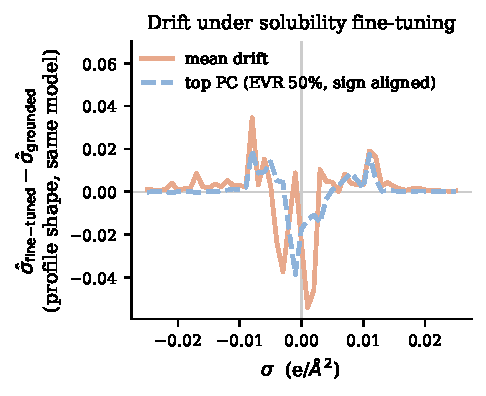
\includegraphics[width=\columnwidth]{figs/fig_compensation_surrogate.pdf}
\caption{The drift solubility fine-tuning imposes on the learned $\sigma$-profile ($n{=}44$
VT-2005-matched molecules): $\hat\sigma$ after fine-tuning minus the \emph{same model's grounded
profile}, not minus the external reference. Shown are the mean drift and its dominant PCA mode,
defined only up to sign and drawn in the mean drift's direction; the legend's EVR is that mode's
explained variance ratio.}
\label{fig:surrogate}
\end{figure}

\paragraph{Dominant mode, and the direct cancellation test.} The dominant drift mode
(Fig.~\ref{fig:surrogate}) transfers area \emph{out of} the nonpolar bins ($\sigma\!\approx\!0$)
and \emph{into} the polar wings: the network represents molecules as more polar than they are.
Whether that shift \emph{cancels} part of $\Bclos$---the input compensating the map, as the
non-identifiability of the split allows (Lemma~\ref{prop:ident})---is the comparison
$\mathrm{MSE}(m,g(\hat\sigma))$ against $\mathrm{MSE}(m,g(\zstar))$ on the same pairs. It does not
support the cancellation reading. Holding the cavity area at its reference value so that only the
profile shape varies, the sole retained end-to-end SLE-trained COSMO-SAC checkpoint gives $18.75$
against $1.47$: on the activity axis its drifted profile is an order of magnitude \emph{worse}
through the same closure, not better. Three limits sit on that number. The checkpoint is the
uncontrolled one, whose departure ($82\%$) is half again the three-seed $51\pm2\%$, so it may not
be representative of the three seeds. The axis is wrong: the drift is produced by the
finite-composition solubility objective and scored here at infinite dilution. The check also has
almost no power in the direction that matters, so it can separate ``no cancellation'' from ``large
cancellation'' but not from ``some cancellation'' (\S\ref{sec:si-mech}). It is the only direct
evidence available, and it is evidence against rather than a clean pass or fail. A second,
independent check on the closure's own axis points the same way: a \emph{more} polar profile moves
$g$ further from $m$ (\S\ref{sec:si-mech}). Both sit on that same infinite-dilution axis, so
neither refutes cancellation in the regime that generates the drift; they remove the one place it
could have been measured, and the cancellation reading remains inferred from the paradox itself. What is established is weaker and still consequential: the model's
``physical'' intermediate is not the molecule's charge distribution, consistent with cautions that
the interpretability of physics-grounded latents is not guaranteed under misspecification
\cite{brynjarsdottir2014,takeishi2021}, and that adapting a representation can itself collapse an
otherwise physically-faithful latent \cite{interno2026}. Its \emph{structure}---low-rank rather
than diffuse---excludes a random collapse but not the structured shrinkage above; the diagnostic
that would separate them is under-resolved here (\S\ref{sec:si-failed-diagnostics}).

\paragraph{What leaves $\sigma$ under-determined by activity.} The freedom that
would make such a cancellation possible is the closure's geometry: at infinite dilution the
activity map concentrates on the one or two hydrogen-bonding directions where the closure is least
faithful (\S\ref{sec:map}). The end-to-end head can therefore move $\sigma$ along the remaining,
low-sensitivity directions at little cost to the fit---the $\sigma$-profile form of
Lemma~\ref{prop:ident}. The Fisher measurement behind that statement, and the two respects in which
it does not settle the question, are in \S\ref{sec:si-mech}; nothing here shows recovery of the
physical profile to be impossible in principle. The sign of grounding turns on \emph{both} axes,
and on which sense of grounding is meant. Freezing the $\sigma$ head at its supervised warm-up
state instead of letting it drift end to end cuts the reference-input penalty by $65\%$
($\Delta\mathrm{MAE}$ from $+0.40$ to $+0.14$ over $n{=}5571$ matched test rows). Those are a
separate matched pair of runs, one base resumed twice with the freeze off and on, and not the
$+0.41$ headline arms of \S\ref{sec:paradox} (\S\ref{sec:si-tables}). A near-physical intermediate
makes the pipeline far more robust to substituting the reference $\sigma$. Supervision alone does
not, however, \emph{flip} the sign here---the penalty stays positive, the closure still being the
low-fidelity COSMO-SAC-2002 and the warm-up $\sigma$ itself only partly physical. The full flip
needs supervision \emph{and} fidelity together, which is what TeNNet-SAC \cite{yang2025tennet} has
and this pipeline does not (\S\ref{sec:intro}).



\subsection{The ceiling is not fixable downstream}
\label{sec:gateb}
% Artifacts: results/e5_sigma_grounding/seed_42/grounded_a_truetrain_residual{,_v2}_predictions.summary.json (Gate B v1 gated-shut / v2 forced-open); model.py correction_force_open_gate.
If the closure binding were merely a bad point estimate, a learned output-space
correction on top of the physics prediction should recover accuracy. It does not.
An additive bounded residual with a learned confidence gate
($\hat y=\hat y_{\text{phys}}+(1-c)\,r$, with $y=\lnx$) leaves the gate
effectively shut (applied residual $\approx0$); forcing it open removes the systematic
\emph{bias} ($+0.45\to+0.06$) but recovers little \emph{accuracy} ($R^2$
$0.236\to0.274$ on the same rows). This is the classical calibration-versus-accuracy
separation: a post-hoc map can fix reliability but not resolution when the
upstream map is misspecified---as expected if the closure, not the estimate, is the binding
constraint. Both arms are seed $42$ only.

\section{Discussion}
\label{sec:discussion}
The result is a cautionary measurement for physics-informed modeling, and it is a measurement about
one of the two operations the word ``grounding'' names. Supervising a learned physical latent on
reference values during training helps ($2.04\to1.85$ in $\lnx$ MAE). \emph{Supplying} those reference
values as an input at inference hurts ($1.85\to2.25$ when substituted at evaluation, $1.80\to1.98$
when the model is allowed to co-adapt), and it hurts because the fixed map that consumes them is
misspecified: when that map is of unknown fidelity---and the standard route does not improve
it---better inputs surface its bias rather than help. Used as an instrument, the decomposition places
the ceiling of the deployed kernel in the closure rather than its inputs, on $477$ activity measurements
over $185$ molecule pairs, scored against the profile database that kernel actually consumes. Whether
that ceiling is a lever depends on the chemistry: the 2002-to-2010 upgrade more than halves the error
on the hydrogen-bonding corner, where the decomposition also localises the defect, and does not lower
it on representative chemistry, a split we resolve on the $57$ pairs the two sets share rather than
leave to the reader. The attribution is an infinite-dilution one: its transfer to the
finite-composition regime the paradox spans is a conjecture supported by in-regime signs (the
more-physics-worse effect on the full $n{=}5608$ set and the chemistry-resolved structure), not a
measured fact.

% Condensed from a full Results subsection; the tables, nulls and controls are in
% App.~\ref{sec:si-blackbox}. Artifacts: results/blackbox/RESULT_study{1a,2,4}*.md via
% scripts/experiments/blackbox_study{1a,2,4}.py on the three checkpoints of \S\ref{sec:paradox}.
% Within-scaffold measure: results/blackbox/within_scaffold_discriminability.json via
% scripts/analysis/run_within_scaffold_discriminability.py on the same three checkpoints.
\paragraph{The unconstrained control does not carry the thermodynamics either.} If the physics arm's
intermediate is a surrogate, the thermodynamics might still be present implicitly in the control,
which is free to represent it. It is not. A ridge probe of the $788$-dimensional pair representation,
fitted on $152$ solutes and scored on $13$ held out, does not recover the measured ideal-solubility
term: $R^{2}=-0.51/{+}0.11/{+}0.03$ across the three seeds, none significant against a $1000$-draw
identity-permutation null, while the same probe recovers the model's own prediction at $R^{2}=0.98$
on the same rows. The permutation null reaches
$R^{2}\approx0.32$--$0.38$ at this sample size, so this bounds the effect at $R^{2}\lesssim0.30$
rather than excluding a weaker one. What it is organised by instead is measurable on
the whole test split, needing no external reference: scaffold identity accounts for
$99.8$--$100.3\%$ of what full molecular identity accounts for, in every seed. The design pins that
ratio near one: only $34$ of the $147$ test solutes share a Bemis--Murcko scaffold with another
($11$ multi-member scaffolds, $8.8\%$ of rows), the raw between-group variance share is
slightly \emph{lower} for scaffold than for solute in every seed ($0.636$ against $0.639$ at
seed~42), and the ratio reaches one only through the two size-matched permutation nulls ($0.022$
against $0.026$), with no interval on the $0.4$--$0.9\%$ raw gap they close. It bounds rather than
measures, and a direct measure on those $34$ solutes sizes what it bounds: two same-scaffold
solutes in a common solvent sit at $0.21$--$0.40$ of the between-scaffold representation distance
across the three seeds ($112$ pairs over $11$ scaffolds; $90\%$ scaffold-cluster intervals inside
$[0.14,0.57]$). Molecules sharing a scaffold are compressed, not unresolved: the representation
buys little beyond scaffold, not nothing. So read, it is consistent with the transfer
limitation of \S\ref{sec:gap}: a test molecule on an unseen scaffold is not a small extrapolation but a point off
the axis along which the representation is organised. Temperature is decodable from this vector at
$R^{2}=0.9997$ yet occupies $3$--$4\%$ of its variance: decodability of a quantity is not evidence
that a representation is organised around it (App.~\ref{sec:si-blackbox}).


\paragraph{What is load-bearing here.} The unit of contribution is the \emph{instrument}, not any single
measurement. Its two ingredients are individually standard: the closure--insufficiency split is a
law-of-total-variance identity, and the sign of grounding's effect follows the model-discrepancy principle
\cite{kennedy2001,brynjarsdottir2014}. What is new is their combination into a usable measurement.
Because a learned physical latent admits an \emph{external oracle}, the two error terms separate on a
\emph{fixed} operator by an identity---with the insufficiency side bounded, not point-identified---and
the resulting sign rule can be tested \emph{a priori} and \emph{bidirectionally}; the pKa domain
supplies that test as an in-distribution sign flip, consistent across splits ($20/20$, $19/20$) and
reaction series ($4/4$, $3/4$; App.~\ref{sec:pka})---with only four series the bootstrap resolves
nothing finer than that agreement, a sign test at $p{=}1/16$ on the pole where grounding hurts. This
oracle-on-a-fixed-operator affordance is what the concept-leakage literature lacks
\cite{parisini2025,espinosa2025leakage}, where the intermediate has no ground truth and leakage is inferred
only indirectly. The solubility results are the instrument's first application, graded in
Table~\ref{tab:claims}; their transfer out of the matched regime is not established.

\paragraph{Why we make no accuracy claim, and what remains after that.} The physics and control arms
were tuned separately---dropout $0.174$ against $0.012$, phase-2 learning rate $8.6\times10^{-4}$
against $8.5\times10^{-5}$, weight decay $4.2\times10^{-5}$ against $5\times10^{-4}$---and no
hyperparameter-matched control was run (\S\ref{sec:si-methods}). A global $\Delta\mathrm{MAE}$ of
$+0.14$ between pipelines whose learning rates differ by an order of magnitude carries no information
about the thermodynamic bottleneck, and neither do the per-solvent-class map, the per-solute-class
map, the novelty inversion or the data-efficiency trend, all of which resolve the \emph{same}
difference along chemical axes. We therefore claim no accuracy result in either direction; those
strata are reported in the SI (\S\ref{sec:map}, \S\ref{sec:data-efficiency}) as hypothesis-generating
descriptions of where two particular pipelines differ, each carrying that caveat, and no conclusion in
this paper rests on them. Running the matched control is the obvious repair and we have not run it.
What survives the confound is every \emph{within-checkpoint} contrast, because there the two sides
share one trained model and one tuning: the $\sigma$-oracle substitution (\S\ref{sec:paradox}), the
closure/insufficiency decomposition, which uses no trained model at all (\S\ref{sec:measure}), the
kernel-fidelity and fitted-residual comparisons, the latent's departure from its reference
(\S\ref{sec:surrogate}), and the output-residual control (\S\ref{sec:gateb}). Separately, and not as
an accuracy claim about the bottleneck: we did not find a configuration in which the physics path
attains a lower error than the control---external state-of-the-art models (FastSolv, SolProp) do no
better on a difficulty-bounding by-solute split (App.~\ref{sec:si-baselines}), and grounding the
crystal factor on external labels did not move the ceiling (\S\ref{sec:e2}). The one place the
physical \emph{structure} helps is temperature extrapolation---as a hypothesis-class property the
trained models do not exploit (\S\ref{sec:supporting}). Two structural facts are consistent with
that: the crystal/activity split is non-identifiable from solubility alone (Lemma~\ref{prop:ident}),
and the activity closure is misspecified where we can measure it (\S\ref{sec:measure}).

\paragraph{When a fixed-closure prior helps versus hurts.} The penalty sign rule (Prop.~\ref{prop:tax})
predicts \emph{when} to expect these negatives: a fixed-closure prior helps only when the estimation
variance it saves exceeds its asymptotic bias $\Delta_\infty$ (both measurable). The ``grounding helps
iff the closure is well specified'' reading is thus a statement about the \emph{bias} channel; even a
true-valued input need not give the lower total error, because a fitted nuisance can be the more
\emph{efficient} estimator---the semiparametric phenomenon by which an estimated propensity
outperforms the known-true one \cite{hirano2003,robins1997}---which Prop.~\ref{prop:tax} carries in
its variance term. The variance benefit is largest at small $n$ and vanishes as data accumulate,
whereas $\Delta_\infty$ is set by the closure; a prior is therefore predicted to hurt precisely in the
mature-data, low-noise, well-covered regime. The fidelity axis can be swept directly outside
chemistry: in a synthetic sweep composing a teacher of known form with a closure of controlled
fidelity $F$, reference inputs hurt monotonically more as $F$ falls (Fig.~\ref{fig:dial};
App.~\ref{sec:dial}), while the pKa closure (App.~\ref{sec:pka}) exercises the sufficiency channel on
real data. Whether grounding helps is shaped by \emph{two} axes---closure fidelity and how the latent
is trained; characterising that plane on real systems is future work.

\begin{figure}[t]
\centering
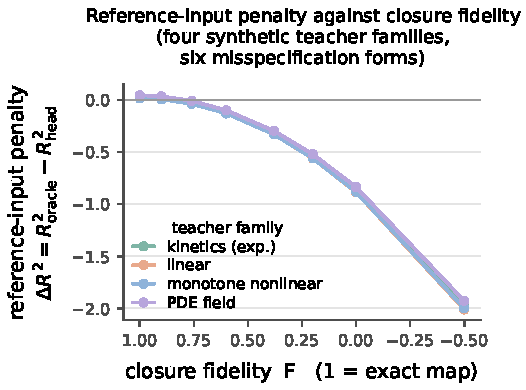
\includegraphics[width=0.78\linewidth]{figs/fig_fidelity_dial.pdf}
\caption{Reproducible closure-fidelity sweep on synthetic, non-chemical teacher functions. As the
closure is made more misspecified (fidelity $F$ falling from $1$; axis reversed), the reference-input
penalty $\Delta R^2=R^2_{\text{oracle}}-R^2_{\text{head}}$ falls monotonically below zero. In this
construction $\Delta R^2$ \emph{equals} $\Bclos$ by design---the free head recovers
$\Ex[m\mid\zstar]$ while $g_F$ is the misspecified map---so the sweep verifies that the instrument
responds to fidelity as constructed; it is a check on the construction, not an independent test of
the hypothesis. The four teacher curves are visually coincident, which shows that the teacher factor
carries no information here rather than that the effect is domain-general; the six misspecification
forms, which do spread, are averaged within each curve and not resolved by the panel, and all $24$
family$\,\times\,$form sweeps are individually monotone. No point is marked for the real closure.
App.~\ref{sec:dial} places it at $F\lesssim0.4$ \emph{only illustratively}---the real-closure-to-$F$
map is a synthetic construction, not a calibrated measurement, and the two $\Delta R^2$ values are
measured on different targets (synthetic $m$ here, $\lnx$ through the SLE solver and crystal head
there).}
\label{fig:dial}
\end{figure}

\paragraph{The novelty inversion (exploratory; not attributable to the bottleneck).} The strata here
resolve the same separately-tuned pipeline difference the previous paragraph declines to interpret,
so none of it is evidence about the thermodynamic bottleneck; we record the pattern because it is
where the sign rule predicts one, and because it names the experiment a matched control should run.
Resolving the penalty by solute novelty, the closure is neutral on the most \emph{novel} solutes
(nearest-train Tanimoto $\le0.3$: $\Delta\mathrm{MAE}=-0.04\pm0.18$) and heaviest on the most
\emph{familiar} ones (Tanimoto $>0.8$: $+0.51\pm0.09$). That is the direction the sign rule would
give if the difference were the prior's, but a separately tuned pair of pipelines can produce it for
reasons that have nothing to do with the prior---a learning rate an order of magnitude apart will
itself sort by how much data a stratum carries---so the agreement is not evidence. The penalty
likewise concentrates in strongly hydrogen-bonding solvents (water $+0.52\pm0.35$) and reverses sign
in the acceptor-dominated amides ($-0.22\pm0.11$) the closure was built for (\S\ref{sec:map}). There
is no multiplicity control across strata families. The diagnostic---measure $\Bclos$ through the
decomposition, read $\Delta_\infty$ off the large-$n$ asymptote, expect the sign to follow---is
\emph{proposed} rather than validated.


\paragraph{On the grades.} The vocabulary is defined in \S\ref{sec:grading} and the claims are
collected in Table~\ref{tab:claims}; one qualification belongs here. Where the clusters are few,
$P\!\to\!1$ states only that every cluster agrees, and we quote the agreement rather than the
frequency---this is why the pKa sign flip is reported as $4/4$ and $3/4$ series rather than as a
bootstrap interval.

% Limitation (i) enlarged-corner numbers: run_b_insuff_decomposition.{match_pairs,evaluate_closure,
% lotv_binning} (res convention, 8 equal-count bins) on notebooks/data/raw/idac_expanded{,_raw}.csv
% against results/sigma_profile_artifact/sigma_profiles.csv; the same call reproduces the deployed
% n=60 corner (MSE 1.4723, B_insuff 0.6180, margin +0.2362) exactly. Expanded: n=115, MSE 1.2553,
% B_insuff 0.4545, margin +0.3463; gas-chromatography-only subset n=100, MSE 0.9250, B_insuff 0.5274,
% margin -0.1298. Provenance of the n=60 pairs: notebooks/data/raw/idac.csv DOI counts 33/20/7 (all
% Chromatography). Corner size audit: results/idac_expansion_audit/summary.json.
% Limitation (i) InChIKey alternative: results/b_insuff/decomposition.json records
% n_pairs_inchikey_match=85, n_solutes_inchikey=46, n_solvents_inchikey=19, computed by
% run_b_insuff_decomposition.py on the same 298 K +-1 K window as the deployed n=60 match.
% Limitation (vi) scaffold geometry: Murcko scaffolds (blackbox_study4.murcko) over the 147 solutes
% of the has_solubility test rows -> 124 scaffolds, 11 multi-member (sizes 2x7, 3, 4, 5, 8) holding
% 34 solutes and 492 of 5608 rows (8.8%).
\paragraph{Limitations.} (i)~The phenomenon and its causal attribution lie in \emph{different
regimes}: the paradox is measured where the model operates (finite composition, all $\gamma$,
$n{=}5608$), but the closure--insufficiency attribution and the latent-departure result are
measured only on infinite-dilution activity data ($n{=}477$ across temperatures, and the $298$\,K,
low-$\gamma$, VT-2005-matched $n{=}60$ and $n{=}44$ sets). Transfer back to the paradox's own regime,
argued above from the
in-regime signs, is a conjecture rather than a measured fact and is the principal open question here.
The matched $n{=}60$ set is also narrowly sourced: under the deployed canonical-SMILES match the
curated IDAC compilation yields $74$ VT-2005-matchable pairs ($60$ at $298$\,K plus $14$
off-temperature), all by gas chromatography and all from three publications, $33$ pairs from one, so
neither a method-stratified nor a source-clustered re-estimate is available on it. A
tautomer-tolerant InChIKey match admits $85$ pairs; we keep the strict rule, which pairs each
measurement with a profile computed for its own tautomer, and have not re-estimated on the looser set.
A broader ThermoML extraction matches $115$ pairs at $298$\,K,
widening the margin from $0.23$ to $0.35$ but \emph{inverting} it to $-0.13$ on the $100$ pairs
labelled gas chromatography, so we do not adopt it \emph{as a replacement corner}; that quality-cut
sensitivity is unresolved at $298$\,K. That is not a verdict on the extraction, which matters because
the representative set is built from the same pull: there the same cut does the opposite, moving the
margin from $+0.95$ to $+1.06$, and the margin also survives clustering on the $15$ source
publications and on the $185$ molecule pairs (\S\ref{sec:measure}(i)). What differs is resolution, not
provenance---at $298$\,K a $15$-row cut moves a margin already inside the design's resolution, on
$477$ rows a $143$-row cut moves one that is not. We therefore use the enlarged pull where it is
stratifiable and keep the strict $n{=}60$ corner where the paradox's own oracle is defined. Because
few drug-like solutes carry a VT-2005 profile, the solubility substitution also falls almost entirely
on the solvent channel; the clean both-channel evidence is on the activity axis. On the corner the
attribution that the misspecification term is the larger rests on a one-sided bound whose margin under
the unbiased within-bin variance is $+0.05$, with clustered-bootstrap support
${\approx}0.7$---below conventional statistical significance and not resolved there. It is resolved on
the $n{=}477$ representative set, which is however not the set on which the paradox's own oracle is
defined. (ii)~$\Binsuf$ is upper-bounded, not point-identified (no
replicates at fixed $\zstar$); the smoothness-free Jensen bound assumes $m$ and $g$ share the $\lngi$
reference state, which we verify (\S\ref{sec:measure}), so the mean offset is genuine decoder bias, not
a units artifact. (iii)~The constant-offset margin is convention-specific and inverts under the
deployed residual-only default; there the separation rests on the convention-independent bound and the
more-physics-worse effect. (iv)~Absolute scaffold
accuracy is encoder-bound but well \emph{above} the inter-lab noise floor ($0.15$--$0.31$ in $\lnx$;
\S\ref{sec:supporting}), so label noise does not explain the ceiling. (v)~The latent-departure
result is three-seed mean$\pm$sd ($n{=}44$; \S\ref{sec:surrogate}); its load-bearing content is the
\emph{sign} and the presence of a transferable shared direction, with the magnitudes
($51\pm2\%$/$72\pm1\%$/$4.1\pm0.5\times$) reported but not stable across revisions of the analysis
pipeline. The two top-two shares in play are distinct quantities: the learned-versus-reference
deviation concentrates $0.399$ in its first two modes---$1.8\times$ a smoothness-matched
phase-randomised null ($0.221$), though below a wrong-molecule null built from real reference profiles
($0.772$; both in \S\ref{sec:surrogate}), and measured on one grounded checkpoint rather than three
seeds---whereas the $72\pm1\%$ isolation drift has no matched null of its own.
(vi)~The probe result on the unconstrained control is bounded by the same
reference scarcity: its crystal-term and temperature tests rest on $13$ held-out solutes and cannot be
enlarged, so the negative is an upper bound at $R^{2}\approx0.30$ rather than a demonstration that no
crystal information is present, and the crystal-slope test is additionally limited by the corpus,
whose empirical slope carries $-\Delta H_{\text{fus}}/R$ at $r=+0.24$. The scaffold-organisation
result needs no external reference, but its two partitions nearly coincide by construction---of the
$124$ scaffolds spanned by the $147$ test solutes only $11$ hold more than one solute, carrying
$8.8\%$ of the rows---so a ratio near one is weak evidence of within-scaffold indistinguishability
(App.~\ref{sec:si-blackbox}). (vii)~The closure-fidelity contrast compares \emph{oracle-input} activity error across kernels, so
$\Ggap$ itself is not measured under a modern closure on either axis, and whether the
\emph{solubility} paradox survives a $2010$/dsp closure is untested. Both require a typed
(donor/acceptor) $\sigma$-profile head trained end to end through the modern kernel, and the
solubility test a UD$\,\cap\,$BigSolDB matched set; we have neither.
(viii)~The two arms were tuned separately and no hyperparameter-matched control was run, so no
$\Delta\mathrm{MAE}$ in this paper---global, per-solvent-class, per-solute-class, novelty-stratified
or data-efficiency---is attributable to the thermodynamic bottleneck (\S\ref{sec:discussion}).
(ix)~The scaffold-leak guard is a property of the released stream builder and not a certified property
of these runs: one $\sigma$-stream build on disk carries $91$ held-out solutes, and per-run stream
provenance was not logged (\S\ref{sec:si-repro}). The paradox contrast is one checkpoint evaluated two
ways and so cannot be generated by such a leak, and DirectGNN uses no stream, but auditability is not
restored by those arguments. (x)~The repository URL, archive DOI, licence and commit hash are
submission-time placeholders in this draft, so a referee cannot exercise the reproduction commands the
Data availability statement describes; several load-bearing numbers---the representative set with its
design and provenance audit, the modern kernel's own-latent floors, the fitted kernel residual, the
estimator grid---are therefore checkable only through code we have not yet been able to release. This
objection stands in full, and the revision has made it heavier rather than lighter, since more of the
verdict now rests on artifacts a referee cannot open.

\section{Conclusion}
\label{sec:conclusion}
Physics-informed models are attractive because they promise both accuracy and interpretability, on the
assumption that grounding their internal quantities in reference physics can only help. That
assumption conflates two operations. Grounding as \emph{training-time supervision} from a reference
database helps here, and by more than the reverse operation costs. Grounding as \emph{inference-time
substitution} of reference values for the model's own hurts, and hurts in the way a misspecified
consuming model predicts. The learned intermediate does not converge to the physical quantity it
represents: it departs from the reference along a direction shared across molecules. Whether that
departure is a compensation for the model's error---which would explain the sign directly---we could
not measure. The one direct check available on retained checkpoints argues against it, but on the
infinite-dilution axis rather than the one that produces the drift and with too little power to
exclude a partial cancellation; we therefore leave it open. The failure is nonetheless diagnosable: an
external reference for the intermediate separates model misspecification from input insufficiency, and
on $477$ activity measurements over $185$ molecule pairs it places the accuracy ceiling of the
deployed COSMO-SAC-2002 kernel in the
fixed model rather than in its inputs, by a margin of $+0.95$ that survives every estimator
configuration we tried. On the $60$ pairs for which the paradox's own reference database is matchable
the same ordering holds only marginally, and under the modern 2010 kernel it is lost.

The practical consequence is that reading a grounded latent as the physical quantity, and supplying
reference values in its place at inference, is justified only to the extent that the downstream
physical model is faithful. When it is not, neither more accurate inputs nor a downstream correction
lifts the ceiling; the remedy must be sought in the model rather than in its inputs, and the standard
upgrade of that model supplies it only on the hydrogen-bonding chemistry it was built for, not on
representative data. Supervising the latent on the
same reference data during training remains worthwhile, and is the sense in which grounding paid here.
The instrument we introduce makes the distinction measurable for any predictor that composes a fixed
physical model over a learned intermediate; whether a latent trained end to end through an imperfect
model generally becomes a compensating surrogate is a testable prediction we state rather than a
result we report.

\section*{Author contributions}
\noindent
%% DRAFT, for both authors to confirm before submission: the roles below are inferred from the
%% work as recorded and are not an agreed statement.
N.~L. Polomoshnov: Conceptualization, Methodology, Software, Formal analysis, Investigation,
Data curation, Visualization, Writing -- original draft.
A.~V. Rudik: Writing -- review \& editing.
%% CRediT vocabulary (use only these 14 names): Conceptualization; Data curation; Formal analysis;
%% Funding acquisition; Investigation; Methodology; Project administration; Resources; Software;
%% Supervision; Validation; Visualization; Writing -- original draft; Writing -- review \& editing.

\section*{Conflicts of interest}
\noindent There are no conflicts to declare.

\section*{Data availability}
All code and the intermediate artifacts needed to regenerate every figure, table and reported number
are available at \url{https://github.com/doctawho42/tgnn-solv} (commit \pending[hash]) under the MIT licence; the model
checkpoints and full per-arm prediction files are deposited at \pending[Zenodo DOI]. \textbf{These are
placeholders in the present draft.} An anonymised repository and an archived snapshot at the commit
that regenerates every reported number will accompany the revised submission; until then the
reproduction commands below cannot be exercised at review, and we record that as limitation~(x). Every
data source is public: the solubility corpus is BigSolDB~2.0 \cite{krasnov2025bigsoldb}, the reference
$\sigma$-profiles are the VT-2005 database, the UD profiles are those of
Ref.~\cite{fingerhut2017} as redistributed with Ref.~\cite{bell2020cosmosac}, the infinite-dilution
activity coefficients are compiled from ThermoML, and the second-domain pKa data are the OPERA
compilation \cite{mansouri2019opera}. The
repository gives the command that reproduces each number from these sources. Two deposited artifacts
carry disclosed caveats, recorded in App.~\ref{sec:si-repro}: the seed-$44$ oracle per-row file is
truncated, and the three-seed surrogate run's per-run split provenance was not logged.

\begin{acknowledgement}
This research received no external funding.
Computations were carried out on commercial cloud services (Google Colab Pro+, Modal, and Google Cloud Platform) using NVIDIA T4 and L4 GPUs.
During the preparation of this work the authors used generative artificial-intelligence
tools (large language models, including Anthropic's Claude) to assist with literature search, drafting
and editing of the text, writing and debugging of analysis code, and generating figures. All content
was reviewed, verified, and edited by the authors, who take full responsibility for the manuscript.
\end{acknowledgement}

\begin{suppinfo}
The Supporting Information contains the notation table; supplementary methods, including the
architecture and the loss weights; proofs of the lemmas and of the grounding-gap theorem; per-arm
tables and the robustness of the decomposition; external baselines and ablations; supplementary
mechanism results; the second-domain pKa analysis; and the full tables of the black-box probe
programme.
\end{suppinfo}

% =====================================================================
% Supplementary Information: proofs, per-arm tables, robustness, mechanism results.
% =====================================================================
\appendix
\section*{Supplementary Information}

\section{Notation}
\label{sec:si-notation}
\begin{table}[h]
\centering
\caption{Notation and coined terms used throughout.}
\label{tab:notation}
\resizebox{\columnwidth}{!}{%
\begin{tabular}{@{}lp{0.62\linewidth}@{}}
\toprule
Symbol / term & Meaning \\
\midrule
$g$ (closure)          & fixed, non-fitted physical map (COSMO-SAC; a Hammett LFER for pKa) \\
$h$ (encoder)          & learned graph network, $x\mapsto z$ \\
$\zstar$, $\hat z$     & reference (oracle) vs.\ learned physical intermediate (the $\sigma$-profile) \\
$m$                    & activity target (experimental $\lngi$) \\
$\Bclos$               & closure misspecification, $\Ex[(\Ex[m\mid\zstar]-g(\zstar))^2]$ \\
$\Binsuf$              & input insufficiency, $\Ex[\Var(m\mid\zstar)]$ \\
$\Gamma$ (grounding gap) & $R_{\mathrm{orc}}-R_{\mathrm{e2e}}$: oracle risk minus best end-to-end risk \\
$\Delta_\infty$ (physics penalty) & asymptotic risk of the physics arm minus the capacity- and budget-matched control \\
full / res             & COSMO-SAC with / without the Staverman--Guggenheim combinatorial term \\
$R_{\mathrm{orc}},R_{\mathrm{e2e}},R_{\mathrm{free}}$ & oracle / best end-to-end / free black-box population risks (they define $\Gamma$) \\
compensating surrogate & a learned $\hat z$ that \emph{cancels} the closure's error instead of matching $\zstar$; here concentrated in a direction shared across molecules, and transferable between them only modestly (\S\ref{sec:surrogate}) \\
$P_{\mathrm{boot}}$    & clustered-bootstrap frequency of $\Bclos>\Binsuf$ on the matched set (a resampling frequency, not a posterior probability) \\
\bottomrule
\end{tabular}}
\end{table}

\section{Supplementary methods}
\label{sec:si-methods}
\paragraph{COSMO-SAC constants.} The differentiable COSMO-SAC layer uses the standard
VT-2005 / Lin--Sandler constants: effective segment area $a_{\mathrm{eff}}=7.5$\,\AA$^2$,
electrostatic-misfit constant $\alpha'=16466.72$\,kcal\,\AA$^4$\,mol$^{-1}$\,e$^{-2}$,
hydrogen-bond coefficient $c_{\mathrm{hb}}=85580$ with cutoff
$\sigma_{\mathrm{hb}}=0.0084$\,e\,\AA$^{-2}$, coordination number $z=10$, and
Staverman--Guggenheim normalisers $r_0=66.69$\,\AA$^3$, $q_0=79.53$\,\AA$^2$; the
$\sigma$-profile grid is $51$ bins on $[-0.025,0.025]$\,e\,\AA$^{-2}$. The segment-activity
fixed point is damped ($\lambda=0.7$) and run for $16$ iterations at train time and $30$
at evaluation.
\paragraph{A usage pitfall in \texttt{cCOSMO} (\texttt{COSMO1} on typed profiles).} Supplying the 2002
kernel with a typed three-profile base produces a silently-wrong result that the library returns without
warning. The reference implementation~\cite{bell2020cosmosac} pairs its 2002 model
(\texttt{COSMO1}) with the single-profile Virginia Tech database; the demonstrated input is one
untyped, Mullins-averaged profile. When \texttt{COSMO1} is instead supplied with a typed three-profile
(Hsieh, \texttt{sigma3}) base --- the configuration that arises when a 2002 and a 2010 arm share one
profile source --- it silently reads the nonpolar channel only, discards the donor and acceptor channels, keeps the
total cavity area as prefactor, and returns a number without error. The prescribed way to recover a
single 2002 profile from the typed set is instead their \emph{sum},
$p=p_{\mathrm{nhb}}+p_{\mathrm{OH}}+p_{\mathrm{OT}}$ (Eq.~9 of Ref.~\cite{bell2020cosmosac}); the
nonpolar-only read is neither that sum nor a documented mode. This single-channel arm scores
$\mathrm{MSE}\ 1.263$ on the matched corner, whereas the fair full 2002 (the same molecule supplied
either to our differentiable layer or to \texttt{cCOSMO} with the full profile placed in the single
nonpolar channel it actually reads) scores $1.757/1.758$. This is an issue for the library maintainers
(a silently-wrong return where an error would be safer), not a defect of any published benchmark.
The kernel arms of \S\ref{sec:measure} are deposited across two artifacts, and which file holds a
value does not follow the set. The dispersion-\emph{off} values ($1.757$ and $0.765$ on the corner, $1.911$ and $1.978$ on
the representative set) are our differentiable layers on each kernel's native profiles
(\texttt{fidelity\_lever\_fair2002.json}). Both dispersion values are \texttt{cCOSMO}'s own
\texttt{COSMO3} call: the corner's $0.785$ from \texttt{closure\_flip\_ci.json}, where the reference
returns no dispersion for the three bromine/iodine pairs and that arm therefore scores on $n{=}57$;
the representative set's $1.855$ from the \texttt{mse\_2010dsp} field of
\texttt{fidelity\_lever\_fair2002.json}, whose corner counterpart in the same file is instead our own
layer's $7.43$. That $7.43$ is the measure of the gap: our transcribed dispersion term is not
validated against the reference, which is why the dsp arm is deferred to \texttt{cCOSMO} throughout.
\paragraph{Crystal head.} $\Tm=100+600\,\sigma(\cdot)\in[100,700]$\,K,
$\dHfus=S_H\,\mathrm{softplus}(\cdot)$; the group-contribution $\Tm$ prior is affine-
calibrated on the train split before entering the head.
\paragraph{Architecture.} The headline COSMO-SAC model uses a message-passing encoder (a shared
backbone with a $2$-layer residual role-specific branch) of hidden width $64$ over $3$ message-passing
layers, on $35$-dimensional node and $8$-dimensional edge features; a set2set readout ($3$ processing
steps) pools each graph, solute and solvent interact through a $3$-layer cross-attention block, and the
$512$-dimensional pair representation $[\,g_s,g_v,g_s\!\odot g_v,|g_s-g_v|\,]$ (dropout $0.012$) feeds
the crystal head, the $51$-bin $\sigma$-profile head, and the parameter-free COSMO-SAC closure. The
full model has $5.40$M trainable parameters---capacity that the in-sample linear probe
($R^2\approx0.76$, \S\ref{sec:supporting}) indicates is not the binding constraint. The DirectGNN
control shares this encoder, interaction, and readout verbatim, and adds a thermometer encoding of
$T$ in place of the temperature dependence the physics arm receives through $\Phi(T)$ and the closure.

\begin{figure*}[t]
\centering
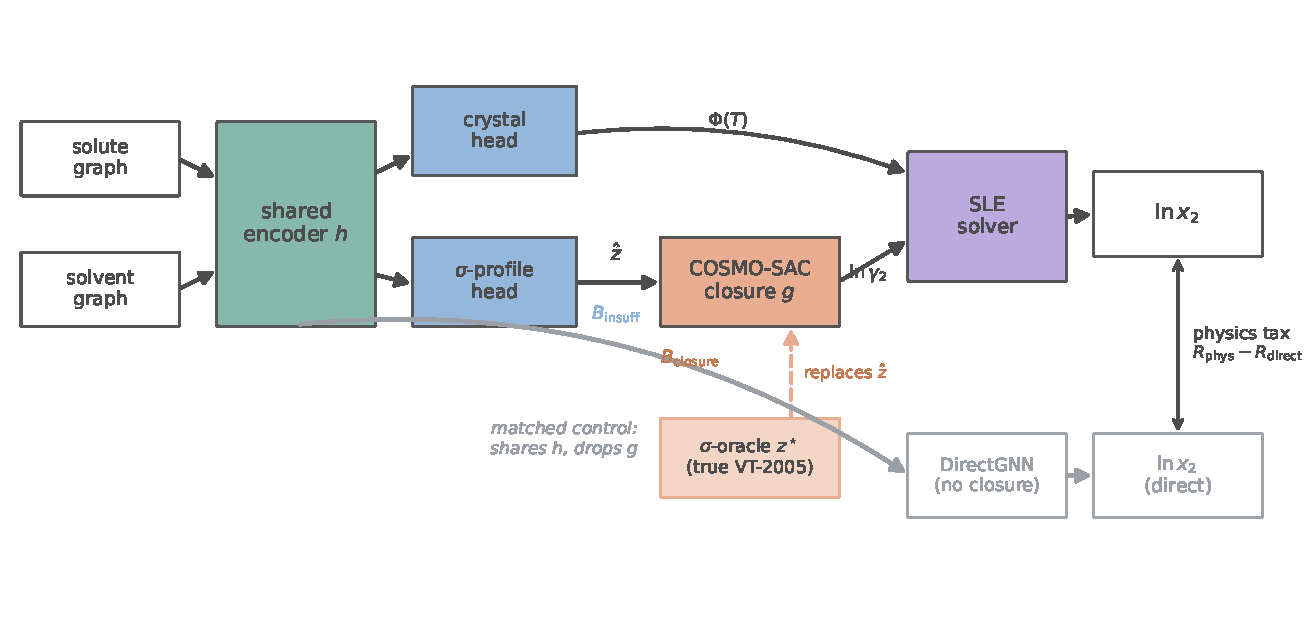
\includegraphics[width=0.82\linewidth]{figs/fig_architecture.pdf}
\caption{The model and the oracle substitution. Solute and solvent graphs pass
through a shared encoder to a crystal head (the ideal term $\Phi(T)$) and a
$\sigma$-profile head; the predicted profile $\hat z$ feeds the fixed COSMO-SAC closure
$g$, which returns $\ln\gamma_2$, and an SLE solver combines the two into $\lnx$. Input
insufficiency $\Binsuf$ enters at the intermediate $\hat z$ and closure misspecification
$\Bclos$ at $g$. The $\sigma$-oracle replaces $\hat z$ with the reference VT-2005 profile
$\zstar$ (salmon). DirectGNN (grey) is the capacity- and budget-matched control---it shares the
encoder but drops the closure; its optimisation settings were tuned separately (\S\ref{sec:framework}).}
\label{fig:arch}
\end{figure*}

\paragraph{Encoder backbones.} The shared encoder has three interchangeable backbones: the
headline message-passing network (MPNN); a hybrid local-message/global-attention graph transformer
(GPS \cite{rampasek2022}); and a physics-channelled variant, Thermodynamically-Informed Message
Passing (TIMP), which splits messages into dispersive, polar, and hydrogen-bonding channels
supervised toward the Hansen parameters to prevent channel collapse. TIMP does not outperform the plain
MPNN across our runs, consistent with the encoder being transfer-limited rather than
expressivity-limited (linear probe train $R^2\approx0.76$, test $R^2\approx0.45$).
\paragraph{Optimisation, and the two arms' settings.} The physics arm uses Adam (weight decay
$5\times10^{-4}$, gradient clipping at $2.0$, batch $64$)
under the three-phase curriculum of \S\ref{sec:methods}: $30$ epochs of auxiliary pretraining (P1),
$70$ of full SLE training (P2), and $10$ of low-rate stabilisation (P3), at learning rates
$2.6\times10^{-4}$, $8.5\times10^{-5}$, and $8.5\times10^{-6}$ respectively. The DirectGNN control
was tuned separately and its settings differ: dropout $0.174$ against $0.012$, P2 learning rate
$8.6\times10^{-4}$ against $8.5\times10^{-5}$, weight decay $4.2\times10^{-5}$ against
$5\times10^{-4}$, gradient clipping $2.54$ against $2.0$, over $110$ P2 epochs equal to the physics
arm's total budget at the same width ($64$) and depth ($3$). Width, depth, batch size and epoch
budget are therefore matched and the optimisation is not, so $\Delta_\infty$ and every per-arm
$\Delta\mathrm{MAE}$ in this paper is a difference between two separately tuned pipelines and is not
attributable to the thermodynamic bottleneck alone (\S\ref{sec:framework}). A
hyperparameter-matched control was not run.
\paragraph{Loss.} The objective is a weighted sum. Of its $32$ registered terms, $17$ carry weight
$0$ by default and never enter training---disabled experimental scaffolding (TIMP channel supervision;
van't~Hoff / temperature terms, $\times7$; Hansen-contrastive terms, $\times5$; descriptor/group priors;
an auxiliary direct-solubility term), released with the code for completeness. The $15$ \emph{active}
terms are below; only the top two groups are load-bearing for the claims, and a loss-simplification
ablation (\S\ref{sec:si-lossablation}) tests which.

\begin{table}[h]
\centering\small
\resizebox{\columnwidth}{!}{%
\begin{tabular}{@{}llr@{}}
\toprule
role & term & default wt. \\
\midrule
task                 & solubility (bin-weighted Huber on $\lnx$)        & $1.0$ \\
crystal grounding    & melting point $\Tm$                              & $0.3$ \\
                     & fusion enthalpy $\dHfus$                         & $0.3$ \\
$\sigma$/act.\ ground.& infinite-dilution $\lngi$                       & $0.5$ \\
                     & finite-composition $\lng$                        & $0.5$ \\
                     & Hansen parameters                                & $0.2$ \\
                     & $\sigma$-profile EMD (grounding stream on)        & $^\dagger$ \\
regulariser          & solubility monotonicity in $T$                   & $0.1$ \\
                     & physics preference                               & $0.1$ \\
                     & adaptive-correction residual                     & $0.01$ \\
                     & NRTL $\tau$                                       & $0.01$ \\
                     & solubility variance                              & cfg \\
control coupling     & DirectGNN NLL                                    & $0.2$ \\
                     & DirectGNN regulariser                            & $0.05$ \\
architecture         & mixture-of-experts balance                       & $0.02$ \\
\bottomrule
\end{tabular}}
\caption{The $15$ active loss terms (non-zero default weight). $^\dagger$The $\sigma$-profile
earth-mover term is active only when the grounding stream is on.
A further $17$ registered terms are disabled (weight $0$). Per-phase weight overrides are pinned in each
run's resolved configuration.}
\label{tab:loss}
\end{table}

\paragraph{Loss-simplification ablation.}\label{sec:si-lossablation}
For a diagnostic result the elaborate objective is a potential confound: the paradox
could be an artifact of loss tuning. We test the opposite---that the paradox and the compensating-surrogate
drift survive a \emph{minimal} objective. Pre-registered before the run: train the end-to-end grounded
arm with only the task ($\lnx$ Huber), the crystal grounding ($\Tm,\dHfus$), and the $\sigma$-profile
warmup, \emph{dropping} the activity-grounding auxiliaries ($\lngi$, $\lng$, Hansen) and every
regulariser, then read the sign of the paradox (oracle vs.\ learned) and the surrogate drift.
Prediction: both persist, because the mechanism is end-to-end training through a misspecified closure,
not the auxiliary terms. Confirmed at the level the ablation measures. The ablation re-measures the
solubility \emph{paradox} (reference minus learned $\lnx$ MAE), the observable effect, not the profile drift
directly: on the full test set it is $+1.13$ (95\% CI $[0.88,1.38]$) under the minimal objective,
\emph{larger} than the $+0.30$ ($[0.20,0.39]$) under the full one. This is the \emph{overall},
solvent-dominated paradox, and it strengthens once the activity-grounding auxiliaries---the only pressure
toward physics---are removed; on the both-reference subset ($n{=}297$ rows over the ${\approx}7$ VT-covered
solutes) the sign in fact reverses ($-0.23$ minimal vs $+0.22$ full), so the ablation is evidence
that the overall observable effect is loss-robust, not subset-level confirmation of the mechanism. It is
\emph{consistent with} the compensating surrogate being intrinsic to end-to-end training through a
misspecified closure rather than a regularisation artifact; it is an implication of the amplified paradox,
not a direct re-measurement of $\lVert\hat\sigma-\sigma\rVert$ under the minimal run (the minimal-loss
checkpoint was not retained, and the larger reference-arm error is consistent with more profile drift but
does not isolate it from closure-path recalibration). The minimal model trains normally (validation
$\lnx$ MAE $1.87$, within $0.1$ of the full-loss base), ruling out a degenerate-training reading
(seed $42$; \texttt{scripts/\allowbreak analysis/\allowbreak run\_loss\_ablation\_analysis.py}).

\section{Proofs}
\label{sec:si-proofs}

\begin{proof}[Proof of Lemma~\ref{prop:ident} (non-identifiability)]
Write $u=1/T$ and $h=\dHfus/\Rgas$, $u_m=1/\Tm$. At infinite dilution and with
$\Delta C_p=0$ the observable is
\[
\begin{aligned}
  \mu(u)=-\Phicry(u)-\lngi(u)&=-h(u-u_m)-(c+d\,u)\\
  &=-(h+d)\,u+(h u_m-c),
\end{aligned}
\]
using $\lngi(u)=c+d\,u$ (affine in $u$ by hypothesis). Thus $\mu$ depends on the
parameters $\theta=(\dHfus,\Tm,c,d)$ only through the pair
$(S,K)=(-(h+d),\,h u_m-c)\in\mathbb R^2$. The activity block spans this plane,
$\partial(S,K)/\partial c=(0,-1)$ and $\partial(S,K)/\partial d=(-1,0)$; hence for
\emph{any} crystal value $(h,u_m)$ and any target $(S,K)$ there is an activity pair
$d=-S-h$, $c=h u_m-K$ reproducing it. The likelihood level set therefore contains the
full two-dimensional family $\{(h,u_m)\}$, so $(\dHfus,\Tm)$ are unidentified.
Equivalently, the crystal score $\partial(S,K)/\partial h=(-1,u_m)$ lies in the span
of the activity columns, so profiling out $(c,d)$ annihilates it and
$\mathcal I_{\mathrm{eff}}(\dHfus)=0$. At finite dilution
$\lng(u)=\lngi(u)\,(1-x_2)^2$ adds $\lngi(u)\,(2x_2-x_2^2)=O(x_2)$, which is not
affine in $u$ because $x_2=x_2(u)$; the crystal score then has a component outside the
activity span of order $x_2$, so $\mathcal I_{\mathrm{eff}}(\dHfus)=O(x_2^2)>0$.
\end{proof}

\begin{lemma}[Class-dependent efficient information]\label{prop:semiparam}
Let the activity nuisance lie in a class $\mathcal H$ with tangent projection
$\Pi_{\mathcal H}$, and let $v=\partial\mu/\partial\dHfus$ be the crystal score.
The efficient information for $\dHfus$ is
$\mathcal I_{\mathrm{eff}}(\dHfus)=\sigma^{-2}\,\lVert v-\Pi_{\mathcal H}v\rVert^2$.
If $\mathcal H$ contains the crystal score's span $\{1,1/T\}$ (a free intercept and slope) then
$\Pi_{\mathcal H}v=v$ and $\mathcal I_{\mathrm{eff}}=0$, recovering
Lemma~\ref{prop:ident}; if $\mathcal H$ is restricted (the slope is known or
constrained) then $\mathcal I_{\mathrm{eff}}>0$ and the Cram\'er--Rao lower bound (CRLB) on
$\dHfus$ is finite. (The melting point $\Tm$ is likewise an unknown crystal parameter, but is
profiled jointly: its score $\partial\mu/\partial\Tm$ lies in $\mathrm{span}\{1\}\subset
\mathrm{span}\{1,1/T\}$, already inside the nuisance tangent whenever the slope is free, so the
dichotomy is unaffected by treating $\Tm$ as free.)
\end{lemma}
\begin{proof}[Proof of Lemma~\ref{prop:semiparam} (class-dependent information)]
This is the semiparametric efficient-score construction \cite{vandervaart1998}
(here finite-dimensional and Gaussian, so equivalently the partitioned-information /
Frisch--Waugh--Lovell identity). With
Gaussian noise of variance $\sigma^2$, parameter-of-interest score
$v=\partial\mu/\partial\dHfus$, and nuisance tangent space $\mathcal T_{\mathcal H}$
(the $L^2$-closure of the span of nuisance scores), the efficient score is the
residual $\tilde v=v-\Pi_{\mathcal H}v$ and the efficient information is
$\mathcal I_{\mathrm{eff}}=\sigma^{-2}\lVert v-\Pi_{\mathcal H}v\rVert^2$. Here
$v=\partial\mu/\partial\dHfus=-(u-u_m)/\Rgas\in\operatorname{span}\{1,u\}$. If
$\mathcal T_{\mathcal H}\supseteq\operatorname{span}\{1,u\}$ then $\Pi_{\mathcal H}v=v$
and $\mathcal I_{\mathrm{eff}}=0$, recovering Lemma~\ref{prop:ident}; if
$\mathcal T_{\mathcal H}$ is a proper subspace not containing $v$ (e.g.\ a fixed
slope, $\mathcal T_{\mathcal H}=\operatorname{span}\{1\}$) then
$\Pi_{\mathcal H}v\neq v$ and $\mathcal I_{\mathrm{eff}}>0$, with a finite
Cram\'er--Rao bound.
\end{proof}

\begin{proof}[Proof of Lemma~\ref{prop:decomp} (decomposition and bounds)]
\emph{(a) Identity.} Split the residual as
$m-g(\zstar)=[m-\Ex(m\mid\zstar)]+[\Ex(m\mid\zstar)-g(\zstar)]$, square, and take
expectations. The squared terms give $\Ex[\Var(m\mid\zstar)]=\Binsuf$ and
$\Ex[(\Ex(m\mid\zstar)-g(\zstar))^2]=\Bclos$. The cross term vanishes: since
$\Ex(m\mid\zstar)-g(\zstar)$ is $\sigma(\zstar)$-measurable, the tower rule gives
$\Ex\big[(m-\Ex(m\mid\zstar))(\Ex(m\mid\zstar)-g(\zstar))\big]
=\Ex\big[(\Ex(m\mid\zstar)-g(\zstar))\,\Ex(m-\Ex(m\mid\zstar)\mid\zstar)\big]=0$.
\emph{(b) Jensen lower bound.} With $\Delta(\zstar)=\Ex(m\mid\zstar)-g(\zstar)$,
$\Bclos=\Ex[\Delta^2]\ge(\Ex[\Delta])^2=(\Ex[m]-\Ex[g])^2$ by Jensen, using
$\Ex[\Ex(m\mid\zstar)]=\Ex[m]$; it requires only that $m$ and $g$ share a reference
state, so that $\Ex[m]-\Ex[g]$ is a genuine mean discrepancy.
\emph{(c) Law-of-total-variance upper bound.} For any binning
$B=\mathrm{bin}(g(\zstar))$, $\sigma(B)\subseteq\sigma(\zstar)$, so conditioning on the
coarser $\sigma$-algebra cannot reduce expected conditional variance:
$\Ex[\Var(m\mid B)]\ge\Ex[\Var(m\mid\zstar)]=\Binsuf$.
\emph{(d) Convention-independence.} $\Binsuf=\Ex[\Var(m\mid\zstar)]$ is a functional of
the law of $(m,\zstar)$ alone and does not involve $g$; hence it is identical across
closure conventions, and any $\mathrm{MSE}(g_1)-\mathrm{MSE}(g_2)$ is entirely
$\Bclos(g_1)-\Bclos(g_2)$.
\end{proof}

\begin{theorem}[Grounding-gap sandwich]\label{thm:gap}
Assume all risks are finite ($m,g(\zstar)\in L^2$; $g$ and each $h\in\mathcal E$
measurable), (A1) the true encoder is representable, $\phi^\star\in\mathcal E$ with
$\zstar=\phi^\star(x)$, and (A2) the intermediate is a lossless bottleneck,
$\Ex[m\mid x]=\Ex[m\mid\zstar]$. Then
\begin{equation}
0\;\le\;\Gamma\;\le\;\Bclos,\qquad
\Gamma=\Bclos-\big(R_{\mathrm{e2e}}-R_{\mathrm{free}}\big),
\label{eq:gap}
\end{equation}
with $\Gamma=\Bclos$ iff $R_{\mathrm{e2e}}=R_{\mathrm{free}}$ (the composed class realizes
the Bayes predictor by distorting the intermediate). In particular a well-specified closure
($\Bclos=0$) gives $\Gamma=0$; hence \emph{under A1--A2}, $\Gamma>0$ certifies $\Bclos>0$.
\end{theorem}
\begin{proof}[Proof of Theorem~\ref{thm:gap} (grounding-gap sandwich)]
Throughout assume $m,g(\zstar)\in L^2$ and $g$, every $h\in\mathcal E$ measurable.
\emph{(a) $\Gamma\ge0$.} By A1, $\phi^\star\in\mathcal E$ is a feasible encoder with
$g(\phi^\star(x))=g(\zstar)$, so $R_{\mathrm{e2e}}=\inf_{h}\Ex[(m-g(h(x)))^2]\le
\Ex[(m-g(\zstar))^2]=R_{\mathrm{orc}}$; the infimum need not be attained. Hence
$\Gamma=R_{\mathrm{orc}}-R_{\mathrm{e2e}}\ge0$.
\emph{(b) $R_{\mathrm{e2e}}\ge R_{\mathrm{free}}$.} Every $g(h(x))$ is
$\sigma(x)$-measurable, and $R_{\mathrm{free}}=\Ex[(m-\Ex(m\mid x))^2]$ is the infimum of
$\Ex[(m-p)^2]$ over \emph{all} $\sigma(x)$-measurable $p$; an infimum over the subclass
$\{g(h(\cdot)):h\in\mathcal E\}$ is no smaller.
\emph{(c) $R_{\mathrm{free}}=\Binsuf$ under A2.} From
$\Var(m)=\Ex[\Var(m\mid x)]+\Var(\Ex(m\mid x))=\Ex[\Var(m\mid\zstar)]+\Var(\Ex(m\mid\zstar))$
and A2 ($\Ex(m\mid x)=\Ex(m\mid\zstar)$, so the two $\Var(\Ex(\cdot))$ terms agree), the two
expected conditional variances agree: $R_{\mathrm{free}}=\Ex[\Var(m\mid x)]=\Binsuf$.
\emph{(d) Sandwich and identity.} By Lemma~\ref{prop:decomp},
$R_{\mathrm{orc}}=\Binsuf+\Bclos$. With (c),
$\Gamma=R_{\mathrm{orc}}-R_{\mathrm{e2e}}=\Bclos-(R_{\mathrm{e2e}}-R_{\mathrm{free}})$, and (b)
gives $R_{\mathrm{e2e}}-R_{\mathrm{free}}\ge0$, so $0\le\Gamma\le\Bclos$; equality
$\Gamma=\Bclos$ holds iff $R_{\mathrm{e2e}}=R_{\mathrm{free}}$. Finally $\Bclos=0$ forces
$0\le\Gamma\le0$, i.e.\ $\Gamma=0$; contrapositively, under A1--A2, $\Gamma>0\Rightarrow\Bclos>0$.
\emph{(e) A2 is necessary for the certificate.} If A2 fails, take $x\in\{a,b\}$ equiprobable,
$\zstar\equiv0$ (so A1 holds), $m(a)=+1,m(b)=-1$, and $g$ with $g(0)=0=\Ex(m\mid\zstar)$ so
$\Bclos=0$; an encoder $h^\dagger(a)=1,h^\dagger(b)=-1$ with $g(\pm1)=\pm1$ gives
$R_{\mathrm{e2e}}=0$ while $R_{\mathrm{orc}}=1$, hence $\Gamma=1>0=\Bclos$. So $\Gamma>0$ alone
does not certify $\Bclos>0$; the decomposition (Lemma~\ref{prop:decomp}) does.
\end{proof}

\noindent The penalty-sign result (Proposition~\ref{prop:tax}, stated in the main text at
\S\ref{sec:tax}) is proved here.
\begin{proof}[Proof of Proposition~\ref{prop:tax} (sign of the physics penalty)]
\sloppy\relpenalty=0 \binoppenalty=0
Write $D(n):=V_{\mathrm{direct}}(n)-V_{\mathrm{phys}}(n)$ and
$\Delta_\infty:=R_{\mathrm{e2e}}-R_{\mathrm{direct},\infty}$, so that
$\mathcal{T}(n)=\Delta_\infty-D(n)$.
\emph{(i)} $\mathcal{T}(n)<0$ exactly when $D(n)>\Delta_\infty$, immediately.
\emph{(ii)} If $\Delta_\infty>0$ and $D(n)\to0$, choose $n^\star$ with $|D(n)|<\Delta_\infty$
for all $n>n^\star$ (possible since $D(n)\to0$); then $\mathcal{T}(n)=\Delta_\infty-D(n)>0$. Monotonicity
of $D$ is \emph{not} required for existence of $n^\star$; it is needed only for the stronger
claim ``$\mathcal{T}(n)>0$ at every $n$,'' which we treat as an empirical observation.
\emph{(iii)} Since $V_{\mathrm{phys}}(n)\ge0$, $D(n)\le V_{\mathrm{direct}}(n)$: the variance a
prior can save is bounded by the control's own estimation variance. As the black box approaches
the aleatoric floor $V_{\mathrm{direct}}(n)\to0$, so $\limsup_n D(n)\le0$; with both estimators
consistent, so $V_{\mathrm{phys}},V_{\mathrm{direct}}\to0$, one has $D(n)\to0$ and
$\mathcal{T}(n)\to\Delta_\infty\ge0$. When the control is asymptotically Bayes, so
$R_{\mathrm{direct},\infty}=R_{\mathrm{free}}$, and A2 holds, then
$\Delta_\infty=R_{\mathrm{e2e}}-R_{\mathrm{free}}=\Bclos-\Gamma$ by \eqref{eq:gap}.
\end{proof}


\section{Per-arm tables and decomposition robustness}
\label{sec:si-tables}
Table~\ref{tab:si-arms} gives the exact per-arm metrics behind
Fig.~\ref{fig:paradox}: three seeds (mean$\pm$sd) on the cross-arm intersection lock
($n{=}5608$, rows supervised and finite in every arm). Both closure families---NRTL and
COSMO-SAC over a learned $\sigma$-profile---trail the DirectGNN control (the physics
penalty); the $\sigma$-oracle (reference VT-2005 profile) is the worst arm, and restoring the
Staverman--Guggenheim combinatorial term makes it slightly worse still---the signature
of a misspecified map (\S\ref{sec:measure}).

\begin{table*}[h]
\centering
\caption{Per-arm scaffold-split metrics (3 seeds, $n{=}5608$ cross-arm lock).
Ordered by MAE.}
\label{tab:si-arms}
\begin{tabular}{lrr}
\toprule
Arm & MAE & $R^2$ \\
\midrule
DirectGNN (no closure)                         & $1.70\pm0.03$ & $+0.42\pm0.03$ \\
NRTL closure                                   & $1.80\pm0.07$ & $+0.34\pm0.03$ \\
COSMO-SAC, learned $\sigma$ (grounded)         & $1.85\pm0.05$ & $+0.33\pm0.05$ \\
\quad $+$ Staverman--Guggenheim combinatorial  & $1.88\pm0.09$ & $+0.32\pm0.05$ \\
COSMO-SAC, ungrounded $\sigma$                 & $2.04\pm0.04$ & $+0.19\pm0.01$ \\
COSMO-SAC, reference $\sigma$ ($\sigma$-oracle)     & $2.25\pm0.02$ & $-0.03\pm0.04$ \\
\bottomrule
\end{tabular}
\end{table*}

% Schedule: configs/cosmo_sac.yaml (freeze_sigma_head_during_sle, warmup 40, 30/70/10 epochs)
% + scripts/experiments/run_e5_sigma_grounding.sh (per-arm invocations).
\paragraph{$\sigma$-head schedule of these arms.} The four COSMO-SAC rows come from three
training runs under one pinned configuration --- $30$ P1, $70$ P2 and $10$ P3 epochs with
\texttt{freeze\_sigma\_head\_during\_sle} on, so the $\sigma$ head's weights are held from P2
onward. The two grounded rows precede that with a $\sigma$ warm-up on the grounding pool (up to $40$
epochs, early-stopped on a held-out tenth of the pool) and interleave the pool through P1; under the
freeze the stream is inactive in P2/P3. The ungrounded row sets warm-up and stream budget to zero,
so its $\sigma$ head is shaped in P1 by the corpus-internal \lngi\ auxiliary loss alone, never by an
external $\sigma$ label, and is frozen from P2 in the same way. The $\sigma$-oracle row is the grounded
checkpoint re-evaluated with $\zstar$ injected, so it shares the grounded schedule exactly. Because
the freeze holds the head and not the encoder that feeds it, the predicted profile is not pinned at
its warm-up value in these arms; we have not run the surrogate isolation (\S\ref{sec:surrogate}) on
these checkpoints, so how far their latent drifted is not measured, and the supervision contrast
quoted there ($+0.40\to+0.14$) is a separate matched pair of runs --- one warm-up-plus-short-P1 base
resumed twice for SLE, with the freeze off and on, on $n{=}5571$ matched rows --- and not these arms.

% Artifacts: results/e5_sigma_grounding/seed_42/{grounded_a_truetrain,channel_swap}_predictions.csv
% (seed 42 only; no seed_43/seed_44 counterpart), scored on the same n=5608 cross-arm lock.
\paragraph{Oracle-application controls: two of the three are single-seed.} Of the three oracle
applications (\S\ref{sec:methods}), only the evaluation-only substitution is a three-seed result.
Training-time injection (MAE $1.98$) and the channel swap (MAE $2.08$) were run at seed $42$ alone,
so their matched comparator is the seed-$42$ learned-$\sigma$ value $1.80$ on the same $n{=}5608$
lock, not the three-seed mean $1.85$ of Table~\ref{tab:si-arms}. Both exceed the worst of the three
learned-$\sigma$ seeds ($1.80/1.92/1.81$), so the direction of both survives a worst-case seed
comparison. The channel-swap margin ($+0.28$) is $2.3$ times the learned arm's full between-seed
range; the training-time margin ($+0.18$) is one and a half times it, so that control fixes a sign
rather than an effect size.

\paragraph{Robustness of the closure/insufficiency separation.} We stress-test the deployed-convention verdict
$\Bclos>\Binsuf$ (\S\ref{sec:measure})---equivalently $\Binsuf<\mathrm{MSE}/2=0.74$ at
$\mathrm{MSE}_{\mathrm{res}}=1.47$---four ways on the $n{=}60$ set.

\emph{(i)~Estimator sensitivity.} The four $\Binsuf$ upper bounds of Table~\ref{tab:decomp}---$0.40$
($k$-NN), $0.62$ (binning/LOTV), $0.56$ (random forest), $0.62$ (ridge out-of-fold)---all fall below the
$0.74$ threshold. The $k$-NN value is the smallest and least conservative input to $\Bclos\ge\mathrm{MSE}-\Binsuf^{\mathrm{up}}$,
so we take the leakage-immune LOTV bound as the headline instead. The LOTV bound bins $g(\zstar)$ and is therefore
finite-sample downward-biased when points per bin are few, which would \emph{inflate} $\Bclos$ favourably;
The two non-binning bounds (RF $0.56$, ridge $0.62$) are immune to that particular per-bin sparsity,
but they do not provide independent corroboration: under random folds every held-out row shares its
solvent or its solute with a training row, so both can borrow strength from a near-twin,
anti-conservatively and in the same direction as the binning (\S\ref{sec:measure}). Blocking folds on
both molecules leaves no informative estimator on this set. The headline should therefore be read as
resting on the leakage-immune LOTV bound alone, not on agreement between three estimators.
The sole non-certifying configuration is a
deliberately aggressive ridge, which lifts $\Binsuf$ to $0.88$ (then $\Bclos\ge0.59<0.88$): a sensitivity
edge, not a refutation.

\emph{(ii)~Leave-one-solvent-out.} Dropping each of the $17$ solvents in turn, the verdict holds in all
$17$ folds under the LOTV bound. Under the random-forest estimator it holds in only $2/17$, because an RF
over-fits conditional variance in $102$ dimensions at $n{=}60$ (its out-of-fold MSE approaches $\Var(m)$),
so its leave-one-out estimate is unstable---an estimator artifact, not a sign flip.

\emph{(iii)~Label noise.} Injecting zero-mean Gaussian noise $\sigma_\eta\in\{0.2,\dots,0.8\}$ into $m$
leaves the $\Bclos$ lower bound stable ($0.84\to0.70$), as expected since
$\Bclos=\mathrm{MSE}-\Ex[\Var(m\mid\zstar)]$ is invariant to zero-mean noise.

\emph{(iv)~Clustered-bootstrap interval.} A solvent-clustered bootstrap ($3000$ resamples of the $17$
solvents, LOTV bound) makes the confidence explicit: the $\Bclos$ lower bound has median $0.93$
(CI$_{90}$ $[0.40,\,1.62]$), and the margin $\Bclos-\Binsuf$ has median $0.36$ (CI$_{90}$ $[-0.22,\,+0.97]$)
with $P(\Bclos>\Binsuf)\approx0.89$ (single-axis; the conservative two-way solute$\times$solvent bootstrap,
which also charges for repeated solutes, gives $\approx0.78$, the value reported in the main text). With
$G=17$ solvent and $41$ solute clusters this small-$G$ regime has optimistic interval coverage, and the
finite-cluster correction acts in the direction of less confidence and non-certification. We
therefore treat the $P$ values as a coarse band, not two-decimal quantities. The separation is
\emph{likely} but not certified at the $90\%$ level under either clustering, which is
why the main text treats it as supporting rather than decisive.

\paragraph{In-regime ($\gamma$-stratified) separation.} The $n{=}60$ measurement is matched at low $\gamma$,
while the paradox spans all $\gamma$. Stratifying the $n{=}60$ set by $\lngi$
tests whether closure-dominance is a regime artifact. It is
not: the verdict $\Bclos>\Binsuf$ (leakage-immune LOTV binning bound) holds in every
stratum and \emph{strengthens} toward higher $\gamma$ (Table~\ref{tab:regime})---in the highest
stratum ($\overline{\lngi}=2.94$, approaching the non-ideal regime) $\Bclos\ge2.69$ exceeds
$\Binsuf\le0.67$ several-fold. The high-$\gamma$ strata are small
($n=17$--$30$ in $102$ dimensions): the law-of-total-variance bound can be pushed toward zero by
too-few-points-per-bin, which mechanically widens the margin exactly where data is thinnest, so
it is the several-fold separations rather than the precise values that carry the
qualitative reading. The bound here bins each stratum into three equal-count bins (against eight in
the main text) and uses the maximum-likelihood within-bin variance, as in the
headline row of Table~\ref{tab:decomp}; recomputed with the unbiased (Bessel) one it rises to
$0.08/0.95/0.81$ across the three strata, so each still separates, but the middle stratum only
marginally ($0.95$ against its own $\mathrm{MSE}/2=0.96$). The $m>\overline{m}$ stratum separates
through its upper (high-$\gamma$) half, and the \emph{isolated} moderate band
($\overline{m}<m\le1.5$) does \emph{not} separate. This is not a counter-example. The total error there
is only ${\approx}0.06$, so $\Bclos\le\mathrm{MSE}\approx0.06$ assumption-free (since $\Binsuf\ge0$),
and there is simply nothing to attribute---near ideality the target is small and the split is
uninformative. We read no closure-quality claim from it in either direction. This supports---but does
not prove---the conjecture that the same closure misspecification drives the all-$\gamma$ paradox.

\begin{table}[h]
\centering
\caption{Closure/insufficiency verdict across $\lngi$ strata of the matched set (deployed
residual-only convention; $\Binsuf^{\mathrm{up}}$ is the leakage-immune LOTV binning bound throughout,
at the maximum-likelihood within-bin variance).}
\label{tab:regime}
\resizebox{\columnwidth}{!}{%
\begin{tabular}{lrrrr}
\toprule
Stratum & $n$ & $\overline{\lngi}$ & $\Binsuf\le$ & $\Bclos\ge$ \\
\midrule
lower $\gamma$ ($m\le$ med.) & $30$ & $-0.40$ & $0.08$ & $0.95$ \\
higher $\gamma$ ($m>$ med.)  & $30$ & $+1.90$ & $0.86$ & $1.07$ \\
high $\gamma$ ($m>1.5$)      & $17$ & $+2.94$ & $0.67$ & $2.69$ \\
\bottomrule
\end{tabular}}
\end{table}

The closure/insufficiency decomposition (full/res conventions; law-of-total-variance (LOTV), random-forest (RF), ridge, and
k\textsc{nn} estimators; solvent-clustered bootstrap; the pyridine stratum) is
tabulated in \S\ref{sec:measure}.

\begin{figure}[t]
\centering
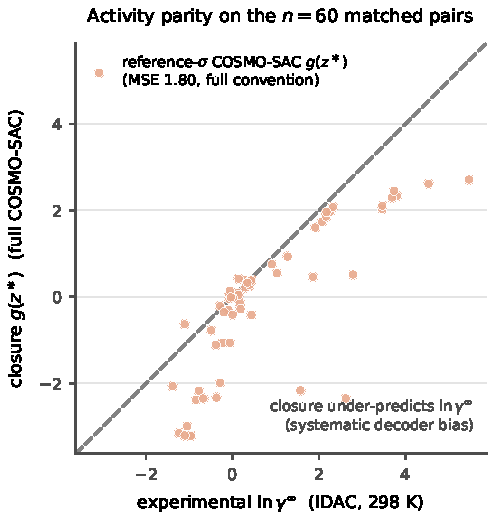
\includegraphics[width=0.72\linewidth]{figs/fig_parity.pdf}
\caption{Activity-coefficient parity on the $n{=}60$ matched pairs. The reference-$\sigma$
COSMO-SAC closure $g(\zstar)$ (salmon) falls below the diagonal at
larger $\lngi$, under-predicting the activity coefficient (MSE $1.80$, full
convention).}
\label{fig:parity}
\end{figure}

\paragraph{The four hedges (full).} The adversarial audit does not invert the verdict
but sharpens its scope:
\begin{enumerate}
  \item \emph{Convention.} The deployed default is residual-only. Under it the
  \emph{constant-offset} (Jensen) lower bound inverts
  ($\Bclos\ge0.43<\Binsuf\le0.62$; it separates only under the full convention,
  $\Bclos\ge0.72$), so that assumption-free bound does not separate under deployment
  (this is the convention-specific row deferred here from Table~\ref{tab:decomp} /
  Fig.~\ref{fig:decomp}), and
  the full-convention margin (the sharpened $\mathrm{MSE}-\Binsuf$ bound,
  $1.27$ vs $0.53$) is a full-COSMO-SAC-only result. What separates under the deployed
  convention is the leakage-immune bound
  $\Bclos\ge\mathrm{MSE}_{\mathrm{res}}-\Binsuf^{\mathrm{LOTV}}\approx0.85>0.62$, which carries
  the headline claim, together with the combinatorial argument above.
  \item \emph{Confound.} The closure error is predominantly a \emph{between-solvent}
  systematic bias ($\sim$64\% of total error); within the largest single-solvent stratum
  (pyridine, $n{=}20$) the closure is nearly correct (stratum MSE $0.07$). Because
  solvent $\sigma$ is part of $\zstar$, these offsets are still decoder error and give an
  independent solvent-conditional lower bound $\Bclos\ge0.89$ (full)/$0.56$ (res).
  \item \emph{Confidence.} Confidence on the full-convention constant-offset
  separation is the solvent-clustered bootstrap $P(\Bclos{>}\Binsuf)\approx0.85$ ($0.83$
  vs the random-forest upper bound, $0.89$ vs the law-of-total-variance bound); we report
  the solvent-clustered scheme rather than the less conservative i.i.d.-pair one because
  solvent dependence dominates. The leakage-immune margin ($0.85$ vs $0.62$) is a
  point estimate. The decomposition is checkpoint/seed-independent (the closure has zero
  learnable parameters).
  \item \emph{Selection/scope.} The 60 matchable pairs are the low-to-moderate $\gamma$
  regime (matched mean $\lngi=0.75$ vs $3.56$ for VT-2005-unmatchable pairs, $t=-7.44$;
  the strongly non-ideal amide-solvent regime is untested because VT-2005 lacks those
  profiles). This narrows scope but is \emph{conservative}, since the untested regime is
  a harder closure test. The target is $\lngi$ at 298\,K, so the numeric ceiling does not
  necessarily transfer unchanged to the finite-composition solubility regime.
\end{enumerate}

\section{External baselines and ablations}
\label{sec:si-baselines}
% Artifacts: results/external_baselines/solute/{fastsolv,solprop_calibrated,solprop_native}_contract_v2/metrics.json.
We evaluated the direct state-of-the-art model (FastSolv \cite{osanloo2024}) and the
physics-informed state-of-the-art model (SolProp \cite{vermeire2022solprop}) on a
by-solute test split (\texttt{test\_solute.csv}, $n\approx10$--$12$k). The two arms are not obtained
the same way, and the difference matters below: FastSolv is retrained on our corpus, whereas SolProp
is the released pretrained thermodynamic cycle---the arm that instantiates the physics---mapped onto
our target by a three-parameter linear recalibration fitted on the training rows, not by retraining.
That cycle is run at $298$\,K on every row, so the temperature of a measurement reaches the SolProp
arm only through the calibrator's temperature term. In $\lnx$ they
reach MAE $1.94$ (FastSolv, $R^2\,0.23$) and $2.34$ (SolProp, calibrated,
$R^2\,{-}0.18$); in $\log_{10}S$, $0.87$ and $1.04$. These are on a \emph{by-solute} split that is
\emph{not comparable} to our scaffold numbers (Table~\ref{tab:si-arms}): they bound the task's
difficulty, not a ranking of the models against one another, so this does \emph{not} establish that our
scaffold-split DirectGNN ($1.70$) outperforms them; a like-for-like scaffold evaluation of the
external models was not run, the deposited external runs being by-solute and pair-random only.
The internal ordering---the physics-informed SolProp trailing the direct FastSolv, the same
ordering we find between our physics closures and DirectGNN---is therefore a
comparison of the \emph{cycle} against a direct model, and it reverses when SolProp's encoder is
instead retrained directly on $\lnx$ with the cycle discarded: that arm reaches MAE $1.63$
($R^2\,0.39$) in $\lnx$ and $0.76$ in $\log_{10}S$ on the $n{=}10{,}287$ rows FastSolv is scored on,
against FastSolv's $1.94$ and $0.87$. We quote the cycle as the physics-informed arm because only it
assembles the separately learned components; the retrained arm measures what discarding the closure
buys on this corpus, not a better physics-informed model. The regime-level reading is that on this corpus no
black box, ours or external, escapes the accuracy ceiling---consistent with the
structural account of \S\ref{sec:discussion}. Per-arm ablations (NRTL vs COSMO-SAC,
combinatorial on/off) are in Table~\ref{tab:si-arms}.

\section{Supplementary mechanism results}
\label{sec:si-mech}
\paragraph{Non-identifiability, empirically (the corrupted twin).} Training a twin model
on data whose crystal labels are corrupted (every $\Tm$ shifted by $+273$\,K) leaves the
\emph{solubility} fit essentially unchanged---$\lnx$ MAE $1.835$ versus $1.812$ on the
corrected data---while the recovered crystal grounding differs by hundreds of kelvin
($\Tm$ MAE $258$\,K versus $45$\,K). Two very different crystal/activity splits produce
the same solubility, which is Lemma~\ref{prop:ident} made concrete.
\paragraph{Crystal grounding on physical labels.} When the crystal head is supervised
on measured melting points it predicts $\Tm$ to $45$\,K MAE, about $4\times$ better than
a Joback group-contribution reference---so the flat downstream result of
\S\ref{sec:e2} is a dose/identifiability effect, not an inability to learn crystal
properties.
\paragraph{The $\Delta C_p=0$ approximation.} The ideal term omits the constant-heat-
capacity correction; a group-contribution audit finds a nonzero $\Delta C_p$ for
$1441$ of $1525$ solutes ($108{,}287$ rows), so this is a bounded model-form
approximation. It cannot produce either headline result. The closure/insufficiency
decomposition is measured on the activity target ($\lngi$ at $298$\,K), where $\Delta C_p$
does not enter at all; and the grounding paradox is an arm-to-arm difference (learned-$\sigma$
vs.\ oracle-$\sigma$) whose two arms share the \emph{identical} crystal term, so any $\Delta C_p$
error cancels exactly in the comparison. It is thus orthogonal to the activity closure, not a
source of the paradox.
\paragraph{Fusion-supervision scarcity.} Direct $\dHfus$ labels are extremely sparse:
$1279$ training rows across $31$ solutes, and essentially none in validation or test.
This is the quantitative basis of the identifiability argument---there is almost no
signal with which to pin the crystal term from data.
\paragraph{The NRTL branch trains (a trainability check).} The asymptotic physics penalty is not an
under-training artifact of the activity branch. In the headline NRTL arm the head produces
solvent-varying interaction parameters---$\tau_{12}$ over the $n{=}8103$ test pairs has mean
$0.97$ and std $2.5$ (range $[-2.6,22]$), far from collapsed---yet the arm still trails the
closure-free DirectGNN ($1.80$ vs $1.70$; Table~\ref{tab:si-arms}). A trained, non-degenerate
activity branch that the control still outperforms is evidence that the penalty is structural, not a
failure to train the branch.
(The core closure-misspecification result---the $\sigma$-oracle and the decomposition---is in
any case training-\emph{independent}: it feeds the reference VT-2005 profiles through the fixed
closure with no encoder optimization, so it cannot be a training pathology.)

\paragraph{Structured temperature extrapolation.} Withholding \emph{temperature} rather
than structure (train at $T\le309.75$\,K, test at higher $T$; $n=3343$), the
affine-in-$1/T$ hypothesis classes extrapolate far better than an unstructured
descriptor regressor (Table~\ref{tab:si-temp}); the van't~Hoff class also predicts the
\emph{direction} of the high-$T$ shift correctly $99\%$ of the time versus $40\%$ for
the random forest. This is a property of the structured hypothesis class---the trained
neural models are weaker than the van't~Hoff baseline---not an accuracy claim for our
model.

\begin{table}[h]
\centering
\caption{Same-pair high-temperature extrapolation ($n=3343$, train $T\le309.75$\,K).
``dir.'' is the fraction of pairs whose high-$T$ shift direction is predicted
correctly.}
\label{tab:si-temp}
\begin{tabular}{lrrr}
\toprule
Model & MAE & $R^2$ & dir. \\
\midrule
per-pair van't~Hoff ($1/T$)     & $0.37$ & $0.89$ & $0.99$ \\
per-pair linear in $T$          & $0.41$ & $0.85$ & $0.99$ \\
per-pair last-low-$T$ hold      & $1.20$ & $0.69$ & $0.01$ \\
RF (Morgan $+\,T$)              & $1.29$ & $0.66$ & $0.40$ \\
per-pair mean                   & $1.46$ & $0.56$ & $0.01$ \\
\bottomrule
\end{tabular}
\end{table}

\section{Supplementary diagnostics and broad negatives}
\label{sec:si-diagnostics}
\subsection{Supporting diagnostics} \label{sec:supporting}

The interpretive claims of the preceding sections are based on a set of controlled diagnostics, each run under a named protocol. We report them here with their exact numbers, including the results that are unfavourable to the physics-informed hypothesis.

% NOISE FLOOR: the derivation, both functionals and every value moved into the article at
% \S\ref{sec:data} on 2026-08-02 (editorial item A3) -- the referees asked for it there and it is
% one of the four things they could not verify without this document. What is left here is the
% part the article does not carry: the upper tail of the per-group distribution, which is what
% says the floor's mean is set by a minority of badly disagreeing systems.
\paragraph{Aleatoric noise floor.} The derivation, the two aggregating functionals and their values
are in the article at \S\ref{sec:data}. One property of the per-group distribution is not: it is
strongly right-skewed, which is why the mean and the median differ by a factor of five. On the
groups backed by two sources the $90$th percentile of the per-group disagreement is $0.42$ \lnx{}
units and the $99$th is $1.41$; on those backed by three, $0.83$ and $3.55$. The floor's
mean is therefore set by a minority of badly disagreeing systems rather than by a broad band, and on
either reading it lies far below the scaffold-split error.

\paragraph{The encoder is transfer-limited, not expressivity-limited.} To separate what the frozen graph embedding can represent from what it transfers out of distribution, we fit a linear probe from the encoder representation onto RDKit descriptors and compare in-distribution and held-out fit. The median train $R^2$ is $0.758$ against a test $R^2$ of $0.448$ ($n=700$ solutes in each partition), a gap of $0.31$. Individual descriptors split sharply: FractionCSP3 transfers well (test $R^2 = 0.96$) while HeavyAtomCount does not ($0.23$). The embedding is expressive enough in sample; what degrades out of distribution is the generalisation of that expressivity across scaffolds. This evidence is suggestive rather than decisive: the sharp per-descriptor spread (FractionCSP3 $0.96$ vs HeavyAtomCount $0.23$) means the train--test gap partly reflects covariate shift in the descriptor \emph{targets} across scaffolds rather than an encoder property alone, and the probe measures descriptor-representability, not task-relevant expressivity directly. It therefore \emph{suggests}---rather than establishes---that a new graph encoder is unlikely to be the main lever for out-of-distribution accuracy, with pretraining and coverage the more likely ones.

\paragraph{Temperature extrapolation.} A structured van't Hoff activity class (log-solubility affine in $1/T$) encodes the correct temperature dependence of \lng{} by construction, and this is apparent when the split withholds temperature rather than structure. Training on measurements at $T \le 309.75$~K and testing at $T \ge 330$~K ($n_{\text{test}} = 3343$), the structured class attains a high-temperature MAE of $0.37$ against $1.29$ for a random forest over Morgan fingerprints plus temperature (in \lnx{} units), consistent with the temperature-aware \lngi{} modelling of \cite{sanchezmedina2023}. This is a property of the structured hypothesis class, not a performance claim for the trained model: the functional form carries temperature extrapolation that a descriptor-plus-temperature regressor does not. Neither is it a claim that our trained arms fail to carry it. The one checkpoint scored on this split is a near-constant predictor whose activity branch never left initialisation, so it separates nothing (\S\ref{sec:si-mech}); what would separate it is a retraining of both arms on this split at the budget used elsewhere here.

% REPLACED 2026-08-06.  What stood here was a single-arm table -- rho 0.511 / top-1 0.477 /
% Kendall 0.436 / nDCG@3 0.732 at n=826 -- computed from
% results/e0_compensation/tgnn_mpnn_test_predictions.csv, an early proxy checkpoint on a
% SUPERSEDED split (826 groups, 5826 rows, against the current 823 and 5608).  It belonged to no
% arm of Fig. 2 and sat one paragraph from the arms a reader would take it for.  It is replaced,
% not annotated, by the paired within-checkpoint contrast of \S\ref{sec:paradox}, which measures
% the same thing on the arms this paper is about.  The retired values are recorded in
% paper/retired_numbers.txt.  The conformal sentence below comes from the same proxy checkpoint
% and now says so.
\paragraph{Ranking and calibration.} Absolute error and decision quality diverge, and within one
checkpoint the divergence has a direction. Table~\ref{tab:ranking} ranks the solvents of each
solute--temperature group of the labelled test rows under the two $\sigma$-profiles of
\S\ref{sec:paradox}: the same weights, the same rows, and only the profile fed to the closure
differing ($\max|\Delta\Phi|=4.2\times10^{-4}$ at the worst of the three seeds, against $4.4$ to
$5.9$ between separately trained arms). With its own learned profile the model orders solvents above
two solute-blind references; with the reference profile substituted it is not distinguishable from
either, on any of the four metrics, at any of the three seeds. Both arms remain far above the
within-group permutation floor, so the substitution does not reduce the ordering to chance---it
reduces it to one that a ranker never shown the solute could produce. Groups are formed on solute
and temperature rounded to $1$\,K, kept when they hold at least three distinct solvents, with
duplicate measurements averaged per solvent. The effective
sample is the $107$ solute clusters, not the $823$ groups, and every interval below is a $95\%$
bootstrap over those clusters.

\begin{table*}[t]
\centering
\caption{Solvent ranking under the two $\sigma$-profiles, on the labelled test rows grouped by
solute and temperature ($823$ groups, $107$ solute clusters, $\ge3$ solvents per group). Both
columns are one checkpoint per seed; only the profile injected into the closure differs.
Per-seed values are $42/43/44$. The last column is the paired per-group difference averaged over
the three seeds, with a $95\%$ cluster bootstrap over solutes; all three per-seed intervals exclude
zero for $\rho$, $\tau$ and nDCG@3, and only seed $42$'s does for top-1, which is why that row is
quoted pooled. The lower block gives each arm's margin over its \emph{own} solute-blind floors---a
floor built from the other arm is not a comparison---and counts, over four metrics $\times$ three
seeds $\times$ two floors, how many of those margins have an interval excluding zero. Each floor is
rebuilt from the predictions of the arm it is set against. One reference-$\sigma$ cell decides that
count on a knife edge and is named so nobody has to rediscover it: nDCG@3 at seed $44$ against its
own shuffled-profile floor is $[-0.0008,+0.0762]$, inside the resampling noise of the boundary
itself, and an independent recomputation places it on the other side. The reference-$\sigma$ count is
therefore $0$ or $1$ according to the bootstrap draw; nothing here turns on which, and the margins
themselves, printed above, are what the reading rests on.}
\label{tab:ranking}
% Width: the tabular must fit \textwidth (504.5 pt) inside table*. At \small with the default
% \tabcolsep it runs 85 pt over, and the stub is where that is won back -- the qualifications
% belong in the caption, not in a row label.
{\footnotesize
\setlength{\tabcolsep}{4pt}
\begin{tabular}{lllr}
\toprule
 & learned $\sigma$ & reference $\sigma$ & reference $-$ learned \\
\midrule
Spearman $\rho$   & $0.592/0.546/0.598$ & $0.365/0.369/0.410$ & $-0.197$ $[-0.282,-0.117]$ \\
Kendall $\tau$    & $0.518/0.469/0.521$ & $0.303/0.306/0.333$ & $-0.188$ $[-0.263,-0.118]$ \\
nDCG@3            & $0.796/0.748/0.792$ & $0.697/0.690/0.698$ & $-0.084$ $[-0.124,-0.043]$ \\
Top-1 accuracy    & $0.586/0.515/0.548$ & $0.447/0.428/0.454$ & $-0.107$ $[-0.192,-0.020]$ \\
\addlinespace[3pt]
\multicolumn{4}{@{}l@{}}{\emph{Margin over its own solute-blind floor} ($\rho$)}\\
shuffled-profile floor    & $+0.120/{+}0.209/{+}0.264$ & $+0.039/{+}0.033/{+}0.079$ & \\
solute-blind label floor  & $+0.240/{+}0.207/{+}0.273$ & $+0.038/{+}0.037/{+}0.080$ & \\
of $24$, excluding zero   & $24$ & $0$ & \\
\addlinespace[3pt]
permutation floor, $\rho$ & \multicolumn{2}{l}{$0.00\pm0.02$, both arms} & \\
\bottomrule
\end{tabular}}
\end{table*}

The shuffled-profile floor gives each group another randomly drawn solute's predictions over the
same solvents, $200$ to $300$ draws; the solute-blind label floor ranks the group's solvents by
their leave-one-solute-out mean measured solubility, which is label-derived and therefore an
optimistic reference. Both are paired per group against the arm they are built from. Two of the
reference arm's twenty-four margins are marginal rather than comfortable---seed $44$ against its
own shuffled-profile floor, $\rho$ $[-0.005,+0.165]$ and nDCG@3 $[-0.001,+0.076]$---so
\emph{indistinguishable from its floor} is the description all twenty-four support, and
\emph{below} it is not. The contrast survives excluding the $16$ groups where some solvent has no
reference profile and the arm therefore runs on a mixture ($807$ groups: $-0.212/{-}0.158/{-}0.172$),
survives a leave-one-solute-out jackknife over the $107$ clusters (ranges $[-0.239,-0.211]$,
$[-0.190,-0.157]$, $[-0.203,-0.171]$), and exceeds at every seed the largest difference between
seed replicates of one arm ($|\Delta\rho|\le0.060$ over nine seed pairs, every interval spanning
zero). Two further readings are not available from it. The floors are built at the prediction
level, not by a forward pass on a permuted profile, so they are faithful to \emph{which} profile
the closure sees and not to how its nonlinearity would answer a profile no molecule has; and the
closure-carrying arm cannot be ranked against DirectGNN here, that difference---DirectGNN minus the
learned-$\sigma$ arm---being $-0.056/{+}0.053/{-}0.040$ by seed, sign-flipping, each interval spanning
zero and each smaller than the seed-replicate spread.

Uncertainty, by contrast, is badly miscalibrated in the native model---a nominal-$90\%$ interval
covers only PICP@90 $=0.13$ of held-out points---but split-conformal wrapping repairs it to $0.92$
empirical coverage at the same nominal level. Those two figures come from an earlier proxy
checkpoint on a superseded split and are a property of an uncalibrated regressor of this family
rather than of any arm of Fig.~\ref{fig:paradox}; the repair is the generic split-conformal
guarantee and does not depend on which arm is wrapped. The ranking signal and the post-hoc
calibrated intervals are the practically usable outputs, even where the point predictions are not
competitive.

\subsection{Identifiability and compensation} \label{sec:ident}

Lemma~\ref{prop:ident} asserts that the crystal/activity split is not recoverable from solubility data alone. Two diagnostics make this concrete. The first is a numerical Fisher audit of the SLE design, computed on synthetic data and independent of any particular activity closure. We evaluate the Fisher information matrix $I$ of the observation model at a reference operating point and read off the conditioning $\mathrm{cond}(I)$ and the Cram\'er--Rao lower bound on the standard deviation of $\dHfus$ under three supervision regimes. Table~\ref{tab:fisher} reports the result at a temperature window of $\Delta T = 40$~K. With solubility measurements only, the design is severely ill-conditioned and the CRLB on $\dHfus$ is roughly $20{,}000$~J/mol, comparable to the quantity being estimated. Adding a direct $\Tm$ label drops the conditioning by nearly two orders of magnitude and cuts the bound to about $3{,}200$~J/mol; supplying $\Tm$ and $\dHfus$ together brings it to about $1{,}700$~J/mol. The ill-conditioning is a property of the design rather than of noise level, and it is closed only by external single-component supervision, which is the mechanism the aux-stream pattern supplies.

\begin{table}[t]
\centering
\caption{Fisher audit of the SLE design at $\Delta T=40$\,K (synthetic,
closure-independent). Solubility alone leaves the crystal parameter
near-unidentified; external single-component labels close the deficiency.}
\label{tab:fisher}
\resizebox{\columnwidth}{!}{%
\begin{tabular}{lrr}
\toprule
Supervision regime & $\mathrm{cond}(I)$ & CRLB $\mathrm{sd}(\dHfus)$ [J/mol] \\
\midrule
Solubility only & $2.3\times10^{5}$ & $19{,}895$ \\
\quad $+\ \Tm$ label & $5.4\times10^{3}$ & $3{,}151$ \\
\quad $+\ \Tm + \dHfus$ & $1.6\times10^{3}$ & $1{,}689$ \\
\bottomrule
\end{tabular}}
\end{table}

Widening or narrowing the temperature window does not rescue the solubility-only case. A $\Delta T$ sweep moves the solubility-only conditioning from $1.7\times10^{3}$ at a wide window to $2.3\times10^{5}$ at $40$~K and to $1.9\times10^{16}$ at $10$~K, so multi-temperature data alone does not resolve the split; the two parameters remain confounded along the ideal-term direction. Restricting the activity slope rather than adding labels helps, but only partially: it cuts $\mathrm{sd}(\dHfus)$ to $8{,}251$~J/mol, still well above the label-supervised regimes. A second, model-side diagnostic must be read with more care, and we keep it out of the load-bearing argument. On the supervised test set, with a group-contribution (Joback) crystal reference, the crystal and activity residuals are strongly anti-correlated ($\mathrm{corr}(\delta\Phicry,\delta\lng)=-0.962$). This is an \emph{accounting artifact}, not evidence of a learned split: the two residuals sum to the (negative) $\lnx$ fit residual, so their correlation tends to $-1$ as the fit improves, a permutation null that destroys any learned coupling still reproduces most of it, and the model's own factors barely co-vary. The large apparent crystal offset is likewise not a usable mis-grounding metric --- it is dominated by reference error, since the Joback reference is physically implausible on these drug-like polycyclics, and capping predicted $\Tm$ at a physical bound collapses the offset from $\approx-7.1$ to $\approx-1.5$.\footnote{Permutation null (learned coupling destroyed) $-0.90$ to $-0.93$; model-factor $\mathrm{corr}(\hat\Phi,\lng)=-0.19$; the Joback reference predicts $\Tm>1000$\,K for a substantial fraction of these polycyclics.} We therefore rest the non-identifiability claim on the reference-free Fisher/CRLB audit above, and relegate the compensation figures to the SI (\S\ref{sec:si-mech}) as a cautionary diagnostic rather than a decomposition-quality measurement.

\subsection{Grounding the crystal factor: a null measured on labels the model already had} \label{sec:e2}

Whether the ceiling lies in the inputs rather than the closure can be tested by grounding a \emph{different} factor---the crystal term---on abundant external data. We trained the identical model without and with an external single-component crystal-property pool of roughly $15{,}000$ melting points ($15{,}427$ molecules), added through the grounding-stream mechanism after excluding any pool solute whose Bemis--Murcko scaffold appears in the validation or test split. Neither the property the pool supplies nor solubility improved on the held-out solutes: melting-point MAE $45.0\to46.6$~K (paired $+1.59$~K over the $n=2518$ test solutes carrying a $\Tm$ label) and $\lnx$ MAE $1.81\to1.88$.

That comparison did not test external crystal grounding, because the pool was barely external. Of its $15{,}427$ molecules, $15{,}082$---$97.76\%$---already carried a $\Tm$ label in the training corpus, $98.2\%$ of them agreeing with the in-corpus value to within a millikelvin (mean $|\Delta|$ $0.07$~K); the net-new contribution is $345$ molecules, $2.24\%$. The two label sets are drawn from the same open melting-point tables, and nothing in the pool builder counts the overlap. Where the pool did carry something new, the crystal head moved. Scored on the pool itself, $\Tm$ MAE falls $35.85\to35.21$~K (paired $-0.636$~K, $95\%$ CI $[-1.09,-0.20]$), splitting into $-0.371$~K $[-0.81,+0.05]$ on the $15{,}082$ duplicated molecules and $-12.233$~K $[-18.25,-6.27]$ on the $345$ new ones---thirty times the movement per molecule on the fraction that supplied information.

Dose was not the constraint. The exported state is the one entering phase 3, after $79$ epochs, by which point the stream had run $632$ optimiser steps---$2.62$ passes over the pool, $93.0\%$ of it seen at least once, the loader reshuffling each epoch---and $240$ of those steps ran at loss weight $1.0$, the phase-1 melting-point weight that an unset stream weight inherits, not at the phase-2 value $0.05$. The downstream half of the null is in turn weaker than its row count suggests: the $+0.065$ $\lnx$ MAE gap is $5608$ rows from $147$ test solutes, and clustered by solute it is $+0.088$ with CI $[-0.127,+0.284]$, crossing zero. Nor is it the activity branch absorbing the crystal branch. Between the two arms the predicted $\Phicry$ differ by $1.25$ ln units per row on average; regressing the predicted $\ln\gamma_2$ on that difference gives a slope of $-0.08$ where full compensation would be $-1$, so $91\%$ of the crystal head's disagreement passes into $\lnx$. The activity-path $\Bclos/\Binsuf$ decomposition does not apply on this path in any case: the crystal ``closure'' is the near-exact ideal-solubility term $\Phi=(\dHfus/\Rgas)(1/T-1/\Tm)$, not a misspecified map.

What the experiment licenses is narrower than a null on external crystal labels, and more useful: a grounding pool has to be measured by its net-new content before it can test anything. This one was scaffold-guarded correctly---none of the $2518$ evaluation solutes appears in it---and was redundant all the same, because the guard protects the estimand and says nothing about what the model already holds. A real test declares the net-new count in advance, the builder reporting it and refusing to run below a floor of a few thousand molecules, which in turn needs a melting-point source disjoint from the one the training corpus itself drew on. Compute is not the obstacle: the grounded arm here was an eight-hour CPU run, so three seeds by two arms is on the order of $50$ CPU-hours. Sourcing the labels is.

\subsection{Chemistry-resolved structure of the physics tax} \label{sec:map}

Across the full test set the two arms are separated by little more than label noise. On the 3-seed scaffold split the DirectGNN control reaches an $\lnx$ MAE of $1.70 \pm 0.03$, while the grounded physics arm (learned-$\sigma$ COSMO-SAC closure) reaches $1.85 \pm 0.05$, for a global $\Delta\mathrm{MAE} = \mathrm{MAE(physics)} - \mathrm{MAE(control)} = +0.14$ (positive meaning the closure adds cost; the per-seed values span $+0.05$ to $+0.25$, so this point estimate is itself only a 3-seed mean, not a tight one; it is computed on unrounded per-seed means, so the rounded $1.70/1.85$ above differ by $0.15$). At this granularity the physics bottleneck is a small, near-noise tax on accuracy. The interesting structure appears only once the error is resolved along chemical axes, where the average tax turns out to be an average over regimes that disagree in sign.

The solvent axis is the sharp one. Binning test pairs by solvent class and recomputing $\Delta\mathrm{MAE}$ per seed (Table~\ref{tab:solvent-map}) shows the cost concentrated in solvents that hydrogen-bond strongly and directionally, precisely the regime in which the COSMO-SAC closure is least faithful and $|\lng|$ is largest. Water carries the heaviest penalty, and the effect decreases monotonically as the donor strength of the class softens. One class inverts the sign: amide solvents, which are aprotic dipolar hydrogen-bond acceptors and therefore closer to the closure's well-specified regime, are the stratum where the tax is smallest and nominally reverses sign ($\Delta\mathrm{MAE}=-0.22 \pm 0.11$ over seeds). We flag this as exploratory rather than a confirmed win: across a family of nine simultaneous solvent-class comparisons the amide interval is an uncorrected per-class pair bootstrap, and the three-seed spread alone does not exclude zero; the halogenated class shows a nominal improvement of similar magnitude but is not seed-robust. The robust reading is the \emph{direction} --- the physics tax shrinks and can turn negative as solvent hydrogen-bond donation weakens toward the acceptor-dominated regime the closure was built for --- not the significance of any single class. This solvent-resolved pattern is the chemistry-resolved shadow of the same synthetic dial we used to vary closure fidelity in controlled experiments.

\begin{table}[t]
\centering
\caption{Per-solvent-class physics tax
$\Delta\mathrm{MAE}=\mathrm{MAE(physics)}-\mathrm{MAE(control)}$ on the scaffold
split (mean $\pm$ sd over 3 seeds; positive means the closure adds cost). The
intervals are uncorrected per-class pair bootstraps across a family of nine
simultaneous comparisons; the two negative (physics-helps) entries are
exploratory, not multiplicity-controlled.}
\label{tab:solvent-map}
\begin{tabular}{lr}
\toprule
Solvent class & $\Delta\mathrm{MAE}$ (mean $\pm$ sd) \\
\midrule
Water & $+0.52 \pm 0.35$ \\
Carboxylic acid & $+0.39 \pm 0.16$ \\
Sulfoxide & $+0.26 \pm 0.24$ \\
Nitrile & $+0.21 \pm 0.19$ \\
Alcohol & $+0.15 \pm 0.14$ \\
Aromatic & $+0.03 \pm 0.63$ \\
Hydrocarbon & $+0.02 \pm 0.50$ \\
Halogenated & $-0.29 \pm 0.36$ \\
Amide & $-0.22 \pm 0.11$ \\
\bottomrule
\end{tabular}
\end{table}

The solute axis tells a compatible but weaker story in prose. Oxygenated solutes ($+0.32$), polyaromatics ($+0.27$), and heterocycles ($+0.17$) are where the closure costs the most, while halogenated-aromatic solutes are roughly neutral. An earlier hypothesis, that the physics path should hurt most on charged and high-$|\lng|$ solutes such as salts, did not replicate once the split was corrected: the charged/salt stratum is neutral at $-0.04 \pm 0.19$. The clean penalty falls instead on ordinary neutral organics, not on the ionic tail we had expected to be hardest.

The most suggestive pattern is a novelty inversion that runs opposite to the usual coverage intuition. Binning solutes into three pre-specified nearest-train Tanimoto-similarity strata, the physics arm is neutral on the most novel chemistry ($\leq 0.3$: $-0.04 \pm 0.18$) and hurts most on the most familiar chemistry ($>0.8$: $+0.51 \pm 0.09$). We flag this as exploratory, not a confirmed effect: the $\pm0.09$ is the spread across three training seeds on the fixed test split, not a within-bin sampling interval over which solutes fall in the stratum, and the Tanimoto binning is one of several strata families we examine (solvent class, solute class, similarity) without multiplicity control. Read as a direction rather than a tested quantity, it suggests the ceiling on the physics path is not coverage or extrapolation but the closure's systematic misfit---masked on novel solutes by the large errors both arms already incur there, and exposed on easy, well-covered solutes where the direct control is accurate enough for a structural bias in the closure to become the dominant residual---consistent with the same closure-misspecification reading as the rest of the paper. A multiplicity-controlled, within-bin-bootstrapped test is left to future work. Read together, the maps say the physics decomposition pays where the closure is misspecified relative to the solvent chemistry, and it can only turn into a win in the narrow acceptor-dominated regime the closure was built to describe.

% The heading used to read "Grounding does not improve accuracy in the low-data regime
% either" -- an accuracy claim in one direction, which Sec. 5 and Table 2 decline to make,
% and which contradicted the caption below it once that caption was made to carry the
% no-claim rule. It names the sweep now, and the text carries the observation with its scope.
\subsection{The data-efficiency sweep, and what survives its confounds}
\label{sec:data-efficiency}
% Artifact: results/data_efficiency/summary.json via run_data_efficiency_summary.py
% over the Modal run (volume tgnn-e5, seed 42); ΔMAE = physics − DirectGNN.
% COMPRESSED 2026-08-20, from about 380 prose words to 190.  Nothing here is attributable -- the
% arms differ in capacity and in optimisation settings, the sweep is single-seed and non-monotone,
% and its endpoint does not reproduce the main comparison -- and the section said so at length.  A
% confound inventory longer than the result it disqualifies invites the question of why the result
% is in the submission at all.  What is kept is the observation that runs AGAINST this paper's own
% reading, and the reason nothing follows from it.  Table~\ref{tab:data-eff} and
% Fig.~\ref{fig:data-eff} are unchanged and carry the rest.
The strongest a-priori case for a physics prior is data scarcity: with few training molecules, an
inductive bias toward the correct factorisation should outperform a data-hungry black box. We test
it by subsampling the training set \emph{by solute} at fractions $0.05$--$1.0$ and training both
arms on the identical subsample (Table~\ref{tab:data-eff}, Fig.~\ref{fig:data-eff}, seed $42$). The
physics arm is worse at every fraction, and against the hypothesis the gap is \emph{smallest} at the
least data ($\Delta\mathrm{MAE}=+0.08$ at $5\%$) --- the one direction in this sweep that favours
the prior rather than this paper's reading of it.

Nothing in the sweep is attributable to the thermodynamic bottleneck, and no accuracy claim is made
from it. The two arms differ in capacity and in the per-arm optimisation settings of
\S\ref{sec:eval}, both are wider than the three-seed arms (hidden width $256$ and $128$ here, $64$
there), the sweep is single-seed with non-monotone physics-arm MAEs, and its endpoint does not
reproduce the main comparison: at fraction $1.0$ it gives $2.98$ against $1.97$ where the three-seed
runs of Table~\ref{tab:si-arms} give $1.7950$ against $1.7022$, a $\Delta\mathrm{MAE}$ an order of
magnitude apart ($+1.01$ here, $+0.09$ there). Both arms are worse than their three-seed
counterparts and the physics arm much the more so ($+1.18$ against $+0.27$ MAE), so the trend
measures how a light per-fraction budget interacts with training-set size at least as much as how a
physics prior does. The one inverting metric is top-1 solvent ranking ($0.42$ against $0.23$ at
$5\%$), which does not translate into lower error.

\begin{table}[t]
\centering
\caption[The data-efficiency sweep]{Data-efficiency sweep (train subsampled by solute, fixed scaffold test,
seed 42). $\Delta\mathrm{MAE}=\mathrm{MAE(physics)}-\mathrm{MAE(direct)}$.}
\label{tab:data-eff}
\resizebox{\columnwidth}{!}{%
\begin{tabular}{lrrrrr}
\toprule
train fraction & \multicolumn{2}{c}{MAE} & $\Delta\mathrm{MAE}$ & \multicolumn{2}{c}{$R^2$} \\
\cmidrule(lr){2-3}\cmidrule(lr){5-6}
(by solute) & physics & direct & (phys$-$dir) & physics & direct \\
\midrule
$0.05$ & $2.28$ & $2.20$ & $+0.08$ & $-0.09$ & $+0.07$ \\
$0.10$ & $2.44$ & $2.07$ & $+0.37$ & $-0.25$ & $+0.15$ \\
$0.25$ & $2.93$ & $1.81$ & $+1.12$ & $-0.75$ & $+0.38$ \\
$0.50$ & $3.12$ & $1.98$ & $+1.14$ & $-0.98$ & $+0.22$ \\
$1.00$ & $2.98$ & $1.97$ & $+1.01$ & $-0.79$ & $+0.22$ \\
\bottomrule
\end{tabular}}
\end{table}

\begin{figure}[t]
\centering
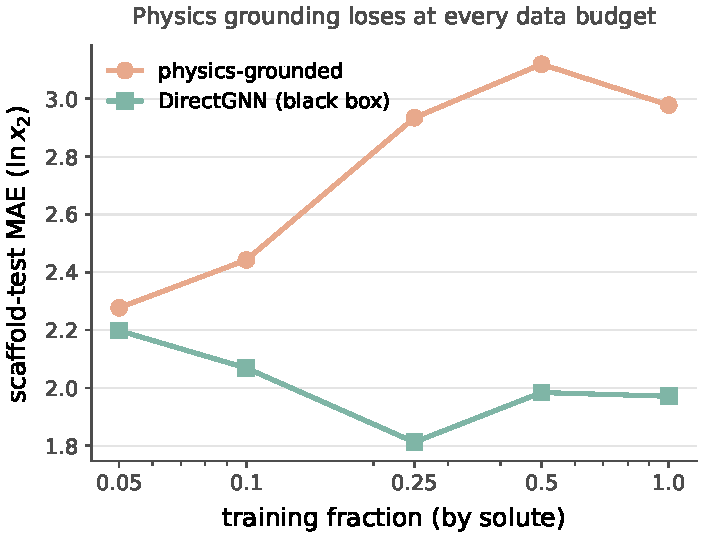
\includegraphics[width=\linewidth]{figs/fig_data_efficiency.pdf}
\caption[The data-efficiency curve]{Data-efficiency curve: scaffold-test MAE of the physics-grounded arm (salmon) and of
DirectGNN (teal) at five training-data fractions, one seed. The plotted values are the MAE columns
of Table~\ref{tab:data-eff}.}
\label{fig:data-eff}
\end{figure}


\section{A second chemical closure: pKa through a Hammett LFER}
\label{sec:pka}
% \S\ref{sec:pka-main} carries the statement of this result in the main text -- what was measured, on
% what, and the two signs. This appendix is the construction behind it and repeats those numbers on
% purpose; keep the two in step if either changes.
The measured result of this section is stated in \S\ref{sec:pka-main}; what follows is the
construction, the estimator and the sweep behind it.
The instrument is not specific to COSMO-SAC. In a second real domain---aqueous $\mathrm pK_a$ of
substituted aromatics---the fixed closure is a Hammett linear-free-energy relationship
$g(\zstar)=\mathrm pK_{a,0}-\rho\,\hammett^\star$ over $\zstar=(s,\hammett^\star)$: the reaction series $s$,
which fixes $(\mathrm pK_{a,0},\rho)$, together with the Hammett substituent constant \hammett,
written with its subscript throughout so that it cannot be confused with the $\sigma$-profile of
\S\ref{sec:framework}, with Hansch--Leo tabulated constants as the
external oracle. The two classic LFER failure modes fall cleanly onto the two channels of
Lemma~\ref{prop:decomp}: \emph{resonance saturation} (a curvature the linear closure cannot
represent) lands in $\Bclos$, while \emph{ortho/steric} effects, absent from the tabulated
constants, are information the intermediate lacks and land in $\Binsuf$. On the OPERA experimental
compilation \cite{mansouri2019opera}---the canonical full set under a uniform, closure-independent
quality filter that drops pre-ionized microstates (\S\ref{sec:si-pka})---this yields a
\emph{measured} fidelity sweep. The clean meta/para series ($n{=}158$) is well specified (RMSE $0.55$,
$\Bclos$ below the insufficiency floor). The degraded pole ($n{=}846$)---an ortho substituent, or one outside the tabulated
list, at some ring position (\S\ref{sec:pka-main})---degrades to
RMSE $2.26$, of which a within-series estimator conditioning on $(s,\hammett^\star)$ places at most $4.5$
of the $5.1$ total in input insufficiency and hence at least $0.6$ in the closure. That estimator is an out-of-fold residual, so
both figures are one-sided, and the a-priori
channel assignment---what the zeroed positions carry and the tabulated constant lacks---is consistent with the
measurement rather than established by it (\S\ref{sec:si-pka}); the sweep is the
near-exact-to-degraded transition. The decisive test is the
same oracle swap as on solubility---the learned $\hat\sigma_{\mathrm H}$ replaced by the tabulated $\sigma_{\mathrm H}^\star$
in the same closure, the sign of the change recorded per stratum---measured \emph{in-distribution} across
$K{=}20$ within-scaffold splits. It \emph{flips}. On the clean meta/para
pole feeding the reference constant \emph{helps} (learned MAE $0.48$ vs oracle $0.315$; oracle better
in $19/20$ splits and in three of the four reaction series): the ceiling there is the noisy learned estimate, not the
closure---a real-data pole on which grounding helps, and an internal positive control. On the degraded pole the
same swap \emph{hurts} (learned $0.83$ vs oracle $1.62$; oracle worse in $\mathbf{20/20}$ splits and in
all four series, gap $90\%$ CI $[{+}0.57,{+}0.95]$): the freely learned $\hat\sigma_{\mathrm H}$ absorbs what
the zeroed positions carry and the tabulated constant lacks. What reverses here is the sign of the grounding penalty; it
reverses through the insufficiency channel---consistent with the one-sided bound above, though not
isolated by it---rather than through the closure-error cancellation of \S\ref{sec:surrogate}: a second
instance of the sign rule, not of that mechanism.
The clustering unit is the Hammett reaction series, of which only $G{=}4$ exist,
so the accompanying bootstrap resolves nothing finer than series-level sign agreement---read as a
sign test on four units, $p{=}1/16$ on the degraded pole and $p{\approx}0.31$ on the clean one---and is
quoted as such (\S\ref{sec:si-pka}).

Both signs are one comparison: the sign of the grounding gap is by construction that of the learned
arm's error against the fidelity-set oracle error, and what a competence sweep adds is that the
oracle side of it does not move with the training budget while the learned side does
(\S\ref{sec:si-pka}). The well-specified pole's threshold (${\approx}0.315$) is never beaten by
the learned arm, so grounding helps at all four budgets swept. The degraded pole's threshold ($1.62$)
is high, so the learned arm beats it, and grounding hurts, across the whole interpolation range
(down to $12\%$ of the data), reverting to helps only under scaffold \emph{extrapolation}, where
$\hat\sigma_{\mathrm H}$ breaks ($2.6{\pm}2.0$) back above the threshold---in the mean over six
splits, three of which still have grounding hurting. The flip is thus a within-distribution, fidelity-driven crossover whose one
scope boundary is that same comparison read where the learned arm breaks. It is the sharp, two-sided form of the penalty sign rule
(Prop.~\ref{prop:tax}); its ``a fitted intermediate can beat the true one'' half is known---plug-in
efficiency under correct specification \cite{hirano2003}, pseudo-true fitting under misspecification
\cite{white1982}---sharpened here into a fidelity-set
threshold. The trained physics-vs-DirectGNN comparison is weaker and is not load-bearing
(\S\ref{sec:si-pka}). On an independent chemical closure the instrument separates a pole where
grounding helps from one where it hurts, each with a sign consistent across splits and series; the full construction,
the estimator validation and the measured sweep are in \S\ref{sec:si-pka} (Fig.~\ref{fig:pka}).

\section{The pKa closure: full construction, measured sweep, and trained comparison}
\label{sec:si-pka}
This section gives the full construction behind \S\ref{sec:pka}: a fixed
Hammett linear-free-energy relationship (LFER) $g(\hammett)=\mathrm pK_{a,0}-\rho\,\hammett$ over the
Hammett substituent constant $\hammett$ (with $\mathrm pK_{a,0},\rho$ the per-scaffold
Hansch--Leo--Taft reaction-series constants), for which Hansch--Leo tabulated constants provide an
external oracle $\zstar$. The analogy is close: as with the $\sigma$-profile through COSMO-SAC, a
learnable physical descriptor is pushed through a fixed, approximate, differentiable map. The two
classic LFER failure modes fall cleanly onto the two error channels of Lemma~\ref{prop:decomp}:
\emph{resonance saturation}---a curvature in $\hammett$ that the linear closure structurally cannot
represent---is a mis-map of a function of $\zstar$ and lands in $\Bclos$; \emph{ortho/steric} field
effects, absent from the tabulated constants, are information the intermediate lacks and land in
$\Binsuf$. The chemical scope is a fidelity sweep: meta/para monosubstituted benzoic acids, phenols,
and anilinium ions are the near-exact ($\Bclos\!\approx\!0$) regime, ortho
(insufficiency-dominated) and polyfunctional the low-fidelity one.

This decomposition is directly visible before any training. Pushed through the fixed Hammett
closure, $p$-nitrophenol reads $\mathrm pK_a\!\approx\!8.3$ against an experimental $\approx7.1$
(and $p$-nitroaniline overshoots similarly): the linear closure is off by $\sim1$ unit exactly
where through-conjugation ($\sigma_{\mathrm H}^-$) breaks it---$\Bclos$ observed in practice.

A controlled semi-synthetic construction on real tabulated $\hammett$ (known ground-truth
channels) validates the estimator and reproduces the paper's central distinction in this second
closure (Fig.~\ref{fig:pka}). Sweeping closure fidelity with a sufficient intermediate, the
grounding gap $\Ggap$ tracks $\Bclos$ (the plug-in estimate recovers the truth to within a few
percent, e.g.\ $0.20$ vs $0.21$, $0.81$ vs $0.81$), the case where Theorem~\ref{thm:gap}'s
proxy is valid. Sweeping the ortho/steric channel with a \emph{well-specified} closure gives
$\Bclos=0$ at every knob while $\Ggap$ rises with the insufficiency fraction, from $-0.035$ at zero
insufficiency through zero near a fraction of $0.25$ to $+0.34$ at $0.7$: at the three fractions
where it is positive it is positive with $\Bclos$ identically zero, which is the pKa realization of
the conflation that makes $\Ggap$ an indicator rather than a certificate. The two negative points
are the same statement in the other direction---a well-specified closure with a nearly sufficient
intermediate leaves the oracle marginally ahead. The oracle-$\hammett$ pipeline
(scaffold-resolved substituent$\to\hammett$ assignment) and this validation extend directly to real
data. On the OPERA experimental $\mathrm pK_a$ compilation \cite{mansouri2019opera} ($7{,}904$
records under the same net-neutral filter), applying the same decomposition to the fixed Hammett
closure yields a \emph{measured} fidelity sweep. On the clean meta/para series ($n{=}158$) the closure
predicts experimental $\mathrm pK_a$ to RMSE $0.55$, with the closure at the input-insufficiency floor:
the leakage-immune lower bound $\mathrm{MSE}-\Binsuf^{\mathrm{up}}$ is $-0.2$ ($95\%$~CI $[-0.4,-0.0]$),
i.e.\ below zero, as a lower bound on the non-negative $\Bclos$ must sit when the LFER predicts as well
as a flexible within-scaffold regressor. There $\Bclos$ is not separately resolvable and is consistent
with a well-specified closure (per-scaffold systematic offsets $\le0.18$). The ortho/heteroaromatic regime ($n{=}846$)
degrades to RMSE $2.26$, dominated by input insufficiency. Here the pKa latent is a \emph{scalar}
Hammett constant, so---unlike the solubility regime---$\Binsuf$ is estimated \emph{directly} rather
than through a coarsening of the closure's argument (\S\ref{sec:decomp}): a within-scaffold
out-of-fold regression estimator gives $\Binsuf=4.5$
($95\%$~CI $[4.0,5.1]$; $\approx89\%$ of the error---the tabulated $\hammett$ carries no ortho
information, exactly the a-priori channel assignment), leaving a closure misspecification
$\Bclos=0.6$ ($[0.3,0.8]$, a stratified within-scaffold molecule bootstrap). Directly estimated is
not point-identified: the estimator is an out-of-fold residual mean square, which is an upper
estimate of $\Ex[\Var(\mathrm{p}K_a\mid\hammett)]$, so $4.5$ is an upper figure and the $0.6$ it
leaves is a lower one---one-sided in the same direction as everywhere else in this paper, and
narrower only because the scalar latent needs no binning (\S\ref{sec:decomp},
\S\ref{sec:pka}). This is the
near-exact-to-degraded transition, measured rather than asserted. This places the pKa closure near the phase-diagram boundary
in its clean regime. \paragraph{Data quality control (uniform, closure-independent).} The trained runs use the canonical
full OPERA set ($7904$ records). A small number of entries are supplied as pre-ionized microstates---an
$[\mathrm{NH}^+]$-protonated aminopyridine at $\mathrm pK_a=-7.78$, a pyrylium $[\mathrm O^+]$, among
others---inconsistent with a neutral-scaffold Hammett assignment, and they degrade the clean pole
(pyridinium RMSE $0.63\!\to\!3.83$). We drop them with one rule, \emph{net formal charge} $\neq0$,
applied uniformly to both strata. It is closure-independent (it never references the oracle residual,
so it cannot be circular) and keeps net-neutral substituents such as nitro $[\mathrm N^+][\mathrm O^-]{=}\mathrm O$.
This removes $5$ of $163$ meta/para rows (restoring the clean pole to RMSE ${\approx}0.55$) and $352$
of $1198$ ortho rows (leaving $846$; the ortho RMSE is essentially unchanged, so the filter does not
manufacture the sign), for $1004$ Hammett-amenable rows.

\paragraph{Evidence for the flip.} We train the physics arm (encoder $\to\hat\sigma_{\mathrm H}\to$ fixed LFER)
on $K{=}20$ stratified $80/20$-within-scaffold splits---a Bemis--Murcko split collapses the meta/para
pole to two ring systems and is unstable---and record the paired per-molecule error against the
deterministic oracle, per stratum. Meta/para: learned MAE $0.48\pm0.09$ vs oracle $0.315\pm0.07$, gap
$-0.165$, oracle better in $19/20$ splits, $90\%$ CI $[-0.28,-0.04]$. Ortho: learned $0.83\pm0.07$ vs
oracle $1.62\pm0.08$, gap $+0.79$, oracle worse in $20/20$ splits, $90\%$ CI $[+0.57,+0.95]$ (both
intervals from the scaffold-cluster bootstrap).

\paragraph{What the two bootstraps do and do not resolve.} We report the sign statements above rather
than the bootstrap $P$ values, because neither bootstrap here carries the resolution a two-decimal $P$
implies. The cluster unit is the Hammett reaction series, and only $G{=}4$ exist (benzoic acid,
phenol, anilinium, pyridinium): the resampling law then has $\binom{7}{4}{=}35$ distinct outcomes and
a finest atom $(1/4)^4{\approx}0.004$, so the cluster-bootstrap $P(\text{oracle worse}){=}1.00$ on
ortho is exactly the statement that all four series means favour the learned arm, and $P{=}0.004$ on
meta/para that exactly one of them does, the other three favouring the oracle. Read as a sign test on
four units those are $p{=}1/16$ and $p{\approx}0.31$; the interval endpoints quoted above are
percentiles of the same $35$-outcome law and are no finer. This is the same small-$G$ caution applied
on the solubility side (\S\ref{sec:si-tables}), where the $P$ values are likewise read as a coarse
band rather than as two-decimal quantities. The split bootstrap adds nothing independent: the $20$
splits resample train/test assignments over the same molecules (each molecule lands in ${\approx}4$
test sets), so it prices split-to-split noise rather than molecule sampling, and with all $20$ ortho
gaps positive it returns $1.000$ by construction---a restatement of the $20/20$, not a second
confirmation. What the flip rests on is therefore the sign consistency across splits and series and
the size of the ortho gap ($+0.79$ against an oracle MAE of $1.62$, ${\approx}49\%$), not on a $P$
value. A leave-one-series-out refit, the estimate that would settle the series-level question at
$G{=}4$, was not run.

\paragraph{The crossover law and its scope boundary.} A competence sweep (train fraction
$\in\{1.0,0.5,0.25,0.12\}$ and, as the low-competence extreme, scaffold extrapolation; six seeds each)
confirms the sign is set by the crossover of the learned error against the fidelity-fixed oracle
threshold. On meta/para the learned arm rises from $0.46$ to $0.98$ as data shrinks but never reaches
the $0.31$ oracle threshold, so grounding helps throughout. On ortho the learned arm stays below the
$1.62$ threshold across the whole interpolation range ($0.85$ at full data, $1.31$ at $12\%$), so
grounding hurts throughout; only scaffold extrapolation, where $\hat\sigma_{\mathrm H}$ breaks to $2.6\pm2.0$,
pushes it back above the threshold and reverts the sign. The flip is therefore a within-distribution,
fidelity-driven crossover, and the extrapolation reversion is predicted by the same law. A trained
physics-vs-DirectGNN comparison agrees in direction overall but has weak absolute errors and an
untuned control; the load-bearing second-domain results are the decomposition above and the
sign-consistent flip.

\begin{figure*}[t]
\centering
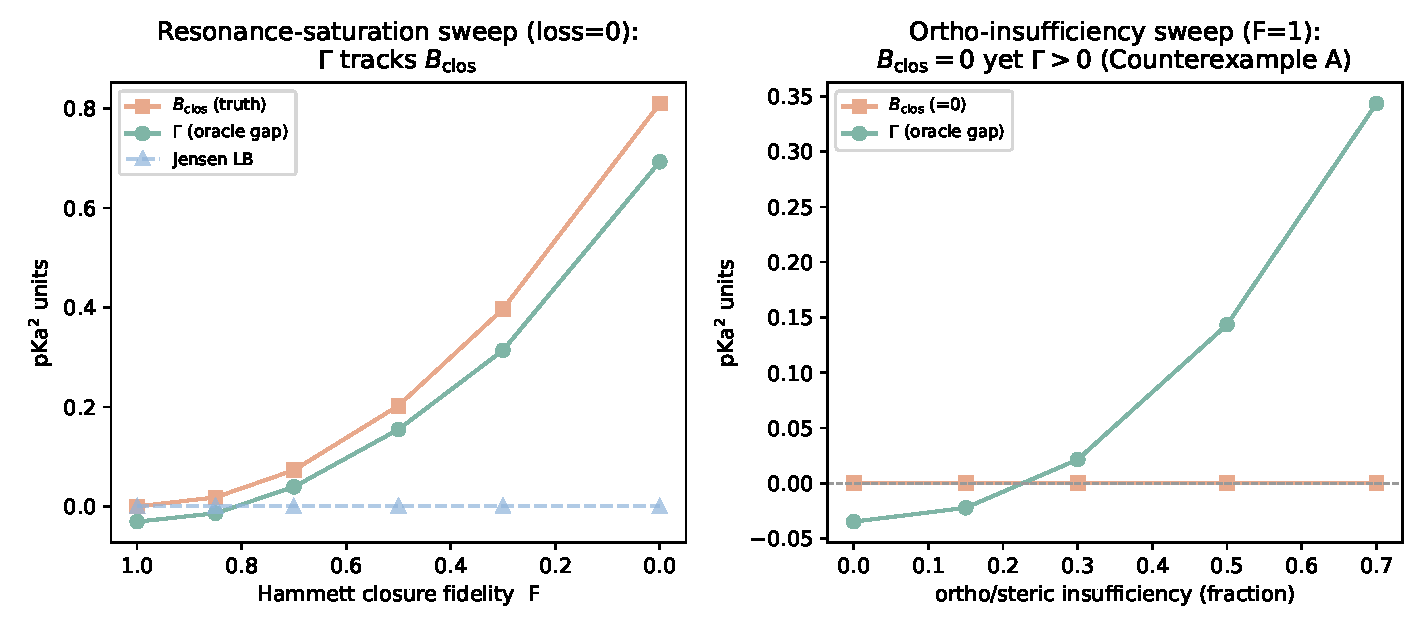
\includegraphics[width=\linewidth]{figs/fig_pka_hammett.pdf}
\caption{pKa through a Hammett LFER on a construction with known ground-truth
channels. \emph{Left:} closure fidelity varied with a sufficient intermediate; grounding gap
$\Ggap$, closure bias $\Bclos$, and the assumption-light Jensen bound. \emph{Right:} an
ortho/steric insufficiency channel varied with a \emph{well-specified} closure; $\Bclos=0$ at each
knob while $\Ggap$ rises with the insufficiency fraction, crossing zero near $0.25$.
Scope: \S\ref{sec:si-pka}.}
\label{fig:pka}
\end{figure*}


\subsection{Diagnostics that do not work, and why}
\label{sec:si-failed-diagnostics}

\begin{figure}[t]
\centering
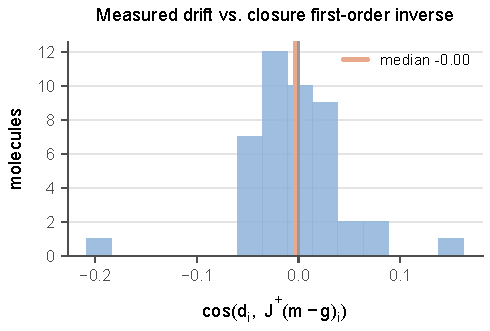
\includegraphics[width=0.82\linewidth]{figs/fig_picard_test.pdf}
\caption{Per-molecule cosine between the measured drift $\hat\sigma-\sigma$ and the first-order closure compensation
$J^{+}(m-g)$; the distribution is centred on zero (median $-0.00$).}
\label{fig:picard}
\end{figure}

\paragraph{The drift is not the closure's signed first-order inverse---but the test is under-resolved.}
A candidate account of the compensating drift is the closure's linear-response inverse,
$\hat\sigma-\sigma\approx J^{+}(m-g(\sigma))$ (with $J=\partial g/\partial\sigma$), predictable a priori
from $J$ before any solubility training. On the matched set the per-molecule drift shows no signed
alignment with $J^{+}(m-g)$ (median cosine $-0.00$; Fig.~\ref{fig:picard}).\footnote{The residual
COSMO-SAC closure runs a segment-activity fixed point, so its autograd Jacobian is numerically unstable
($\lVert\partial g/\partial\sigma_{\text{solvent}}\rVert\!\sim\!10^{15}$ at infinite dilution); $J$ is
computed by finite differences on the converged closure.} We read this as a signed negative only, and do
not build on it, for two reasons intrinsic to the test. First, the matched set is sparse (median one
pair per molecule), so each per-molecule Jacobian subspace is one-dimensional and the dimension-matched
row-space controls are uninformative---a resolved direction common across molecules makes a molecule's
``own'' and ``other'' subspaces coincide. Second, and more fundamentally, the single-pair $J^{+}(m-g)$
is a poor \emph{estimator} of the first-order compensation: the activity Fisher is near rank-one
($\mathrm{PR}\approx1.4$ of $51$, \S\ref{sec:surrogate}), so the closure's first-order inverse is
ill-posed along all but one direction. A null here is therefore uninformative about whether the drift is
first-order, not evidence that it is not. The load-bearing claim is the under-determination of $\sigma$
by activity (\S\ref{sec:surrogate}), not the geometry of the drift.

The instrument behind \S\ref{sec:surrogate}---the rank of the activity Fisher $J^{\top}J$
($J=\partial\lngi/\partial\sigma$), read as a participation ratio
$\mathrm{PR}=(\sum_i\lambda_i)^2/\sum_i\lambda_i^2$---is computationally inexpensive and oracle-free, which
is its appeal for probing any physics-grounded latent. It is also easy to misread in three ways that inflate a null or a rank
in the flattering direction, silently; we record them because the corrections are not obvious.

\paragraph{(i)~Finite differences inflate the participation ratio.} $\mathrm{PR}$ is a \emph{tail} statistic,
governed by the small eigenvalues. A closure evaluated by an unrolled fixed point carries a small,
step-\emph{independent} gradient noise (from the convergence tolerance, not truncation), so central finite
differences lift the exactly- and near-zero eigenvalues onto a floor and $\mathrm{PR}$ rises. On the
differentiable COSMO-SAC-2002 layer, autograd and finite differences on \emph{identical} profiles give
$\mathrm{PR}=1.00$ and $1.25$---a $25\%$ inflation from noise alone, though the per-gradient cosine is $0.995$
(the direction is right, the tail is not). It is worse on a typed ($3\times51$) profile basis: a closure that
ignores the typing (2002) has $102$ exactly-redundant coordinates that finite differences decorrelate into a
spurious floor, inflating its $\mathrm{PR}$ from $1.0$ toward $2.0$, while a closure that uses the typing
(2010) has no such redundancy---so the same step inflates the two \emph{asymmetrically} and can manufacture a
rank ordering with no physical content. \emph{Autograd is the appropriate instrument where the closure is
differentiable; with only finite differences, $\mathrm{PR}$ is interpretable against a known-rank or
permuted control, never absolutely.}

\paragraph{(ii)~``Own vs.\ other'' controls are powerless when the resolved direction is common.} A
dimension- and smoothness-matched control aligns a molecule's drift against its own predicted compensation and
against other molecules'. It has power only if the predictions differ. But when the aggregate Fisher is
rank-one (\S\ref{sec:surrogate}) the resolved direction is \emph{common}, so ``own'' and ``other'' point
almost the same way and the diagonal must sit inside the null---$p\approx0.5$ regardless of the truth. On the
matched set sparsity compounds this: a median of one pair per molecule makes each per-molecule Jacobian
subspace one-dimensional, so ``own'' and ``other'' subspaces coincide exactly. \emph{A control's null is
interpretable only once its power is established: if the compared predictions have median cosine near one,
the test cannot reject.}

\paragraph{(iii)~Energy-in-subspace baselines need the effective rank and a cluster null.} A random zero-mean
vector in $D$ dimensions places $k_{\mathrm{eff}}/(D{-}1)$ of its energy in a subspace of \emph{effective}
rank $k_{\mathrm{eff}}$ (the participation ratio of its singular values), which for near-collinear Jacobian
rows is far below the nominal row count. On the matched set the per-molecule subspace is effectively
one-dimensional, so the baseline is ${\approx}2\%$ and the observed $5.5\%$ is a two-to-threefold
\emph{enrichment}, not the ``no concentration'' a raw own-versus-other equality suggests: own equals other
because both one-dimensional subspaces are the same common direction, not because the drift avoids the
resolved one. And with that direction common, $N$ enriched molecules are not $N$ independent draws---the
enrichment needs a cluster null (\S\ref{sec:measure}), without which its significance is over-stated by
$\sqrt{N/N_{\mathrm{eff}}}$. We therefore report the $5.5\%$ as evidence in neither direction. \emph{The
baseline must be set by effective rank, and the null clustered by the shared direction.}

Each failure turns a soft spectral quantity into a hard structural claim---the mode the surviving
statements of \S\ref{sec:surrogate} avoid by carrying their null model and a power check inline.

\section{Data provenance and reproducibility}
\label{sec:si-repro}
\paragraph{Sources.} Solubility: BigSolDB~2.0 \cite{krasnov2025bigsoldb}. Crystal
$\Tm/\dHfus$: an open melting-point pool plus a group-contribution prior. True
$\sigma$-profiles: the VT-2005 database (ingested to
\texttt{sigma\_profiles.csv}, $1432$ compounds, with the COSMO cavity volume
$V_{\mathrm{cosmo}}$ for the combinatorial term). These are quantum-chemically computed for a
single reference conformer and protonation state; mismatch to the experimental measurement
conditions is noise in $\zstar$ that inflates $\Binsuf$, but under a Berkson-type displacement it
also loads onto $\Bclos$ through the curvature of $g$, so we treat it as an unsigned limitation and
\emph{not} as conservative for the closure-dominance verdict (\S\ref{sec:measure}). Infinite-dilution
activity coefficients: ThermoML. Enlarging the reference $\sigma$-profile set would not materially
grow the matched activity corner: of the $298$\,K ThermoML IDAC pairs, only two solutes lack a VT-2005
profile while their solvent has one---the binding constraint is joint IDAC$\times$profile coverage, not
profile availability. What does enlarge the corner is a broader extraction on the IDAC side: the
expanded ThermoML pull released with the code matches $115$ pairs at $298$\,K, which we do not adopt
because its verdict is quality-cut sensitive (\S\ref{sec:discussion}).
The corner is matched to VT-2005 by RDKit canonical SMILES on solute and
solvent, the rule the deployed $\sigma$-oracle itself uses; matching by InChIKey instead admits $85$
pairs over $46$ solutes and $19$ solvents at $298$\,K in place of $60/41/17$ (both counts are recorded
in \texttt{decomposition.json}). We keep the stricter rule so that the $\zstar$ charged against each
label is the profile the deployed pipeline would supply, rather than one imported across a tautomer or
protonation variant---the same mismatch that makes the reference imperfect above. The decomposition
was not re-estimated on the InChIKey-matched set; whether the verdict moves on those $25$ extra pairs
is untested. Second-domain pKa: the OPERA experimental compilation
\cite{mansouri2019opera} (\texttt{pKa\_QR.sdf}, $7904$ QSAR-ready records, public-domain US EPA;
cited, not redistributed); the uniform net-formal-charge filter reduces this to the $1004$
Hammett-amenable rows ($158$ meta/para, $846$ ortho/heteroaromatic) analysed in \S\ref{sec:si-pka}. The Bemis--Murcko scaffold split follows the main text; because the seeded
split is not stable across pipeline versions (\S\ref{sec:framework}), every number in this paper is
computed on a \emph{single} committed split, whose molecule-level hash is recorded with the released
artifacts.\footnote{The three-seed surrogate isolation (\S\ref{sec:surrogate}) was produced on a
separate run whose per-run split provenance was not logged; its matched set is the same $n{=}44$
molecules, derivable from the committed split independently of the model, so it is consistent with the
reported split. We record the split hash in the runner so future runs are auditable directly.}
Melting-point tables are auto-detected as $^\circ$C or K to avoid a $+273$\,K double-conversion.
% Artifact: notebooks/data/processed_sigma_aux_stream/summary.json (exclude_scaffolds_from points at
% a debug split; n_excluded_scaffolds 48 vs 2702 in the crystal stream's summary.json); guard in
% scripts/data/build_sigma_profile_aux_stream.py.
\paragraph{Grounding-stream provenance, and one build that violates the guard.} The
$\sigma$-stream builder drops any pool molecule whose Bemis--Murcko scaffold appears in the
validation or test split and aborts rather than proceed when a split file is missing; a correct
build retains $1319$ of the $1427$ VT-2005 molecules that parse into the pool. The stream file was
subsequently rebuilt with the exclusion pointed at the splits of a small debug dataset: it carries
$1425$ rows, of which $106$ ($99$ train, $7$ validation) have a scaffold in the real
test$\,\cup\,$validation union of $2702$ scaffolds. The overlap is not confined to scaffold
relatives: $91$ of those $106$ rows are themselves held-out solutes by canonical SMILES --- $65$
test solutes and $26$ validation solutes --- and the correctly guarded build leaves none of them.
The crystal stream's build on disk
records the correct $2702$-scaffold exclusion, so among the streams feeding the runs reported here
the defect is confined to the $\sigma$ one. Per-run stream provenance was not logged, so the
artifacts cannot certify which build fed which arm. The rebuilt file postdates every prediction file
behind Fig.~\ref{fig:paradox} and Table~\ref{tab:si-arms} and predates the two single-seed
oracle-application controls (\S\ref{sec:si-tables}) and the output-residual arms
(\S\ref{sec:gateb}); that ordering is consistent with the headline arms having used the guarded
build and the later controls the leaking one, but these are timestamps on local copies of
cloud-run outputs and settle nothing on their own. Three facts bound what the leak can do. It is
common-mode across the paradox contrast, the learned-$\sigma$ and $\sigma$-oracle rows being one
checkpoint evaluated two ways, so it cannot generate the gap between them; DirectGNN uses no
grounding stream, so a leak can only flatter the physics arm that loses to it; and on the $n{=}44$
matched set of \S\ref{sec:surrogate} a correct guard would have removed one molecule (piperidine).
What it does compromise is auditability, and with it the reach of the split guarantee: an arm
trained on that build would have had reference $\sigma$-profiles --- though no solubility labels ---
for $65$ test solutes, and the guarantee stated in \S\ref{sec:methods} is therefore a property of the
released builder rather than of every stream file we trained on. Closing this requires hashing each
stream build beside the split hash, which was not done for these runs.
\paragraph{Compute ledger.} The headline $\sigma$-grounding comparison
(Fig.~\ref{fig:paradox}, Table~\ref{tab:si-arms}) is a full-corpus GPU run (three seeds);
the closure/insufficiency decomposition (\S\ref{sec:measure}), the
Fisher audit (\S\ref{sec:ident}), the noise floor, the encoder probe, and the
temperature and mechanism diagnostics of \S\ref{sec:si-mech} are CPU-reproducible from
committed artifacts. Each figure and table names the script that regenerates it from
\texttt{results/}; large prediction CSVs and model checkpoints are deposited separately
(\pending[Zenodo DOI]) rather than in the repository.
\paragraph{Seeds and determinism.} Controlled comparisons use seeds $\{42,43,44\}$ and
are reported on a cross-arm intersection lock (rows supervised and finite in every arm); the
surrogate isolation (\S\ref{sec:surrogate}) uses seeds $\{0,1,2\}$; the training-time and
channel-swap oracle controls and the output-residual arms (\S\ref{sec:gateb}) are seed $42$ only.
The decomposition is seed-independent
(its closure has no learnable parameters). One artifact caveat: a save-time bug truncated the released
per-row prediction file for the seed-$44$ oracle solubility arm to $295$ rows, a small fraction of the
test set. The three-seed headline summaries (Fig.~\ref{fig:paradox}, Table~\ref{tab:si-arms}) were
aggregated at run time, before that file was written, so they are unaffected; only the one on-disk
artifact is partial, and any per-row re-analysis of the solubility arms therefore uses the two complete
seeds ($42,43$). The learned-$\sigma$ and DirectGNN solubility files and the activity-level
($n{=}60$, $n{=}44$) artifacts are complete for every seed.

\section{Black-box probe programme: full tables}
\label{sec:si-blackbox}
% Artifacts: results/blackbox/*.md and *.json; scripts/experiments/blackbox_study{1a,2,4}.py.
All three studies use the same current-split DirectGNN checkpoints (seeds $42/43/44$, test MAE
$1.749/1.674/1.684$) whose manifests pin the train/val/test SHA-256 to the split on disk. Every
figure is CPU-computed; no number here required a GPU.

\paragraph{Crystal-term decodability.} Probe fitted on $152$ solutes / $14{,}348$ rows,
scored on $13$ held-out solutes / $527$ rows, solute overlap zero. $\Phi^{*}$ is $92.2\%$
between-solute variance, so the effective $n$ is $13$ clusters.

\begin{table*}[t]
\centering\footnotesize
\begin{tabular}{lccccc}
\toprule
seed & $R^{2}$(model) & perm.\ $p$ & jackknife range & sign flips & top-3 leverage \\
\midrule
42 & $-0.506$ & $0.894$ & $[-1.151,\,-0.228]$ & $0/13$ & $56.2\%$ \\
43 & $+0.111$ & $0.055$ & $[-0.286,\,+0.333]$ & $3/13$ & $59.8\%$ \\
44 & $+0.027$ & $0.177$ & $[-0.253,\,+0.237]$ & $6/13$ & $57.2\%$ \\
\bottomrule
\end{tabular}
\caption{Crystal-term decodability per seed, with the permutation null, the drop-one-solute jackknife and the leverage carried by the worst solutes.}
\end{table*}

\noindent Controls: positive---model's own prediction $R^{2}=0.980$, temperature $R^{2}=0.9997$;
negative---random target $-0.0006$, molecule-blind constant profile $-0.015$, raw RDKit
descriptors $-0.514$ (set A) and $-0.928$ (set B). Null $p_{95}=+0.105/+0.117/+0.096$ and
$\max=+0.316/+0.380/+0.346$ over $1000$ draws.

Two features of this table bear on how such probes should be
read. First, the between-seed spread ($0.616$ range, sd $0.334$) exceeds every individual value:
a single-seed run would have been unreadable, and seed $43$ alone would have read as a
near-miss. Second, a decision rule of the common form
$R^{2}(\text{model})-R^{2}(\text{raw})\ge0.10$ would have declared success here on all three
seeds under descriptor set B---including seed $42$, whose probe is worse than a molecule-blind
constant---and on two of three under set A. The subtrahend is an unregistered analyst choice
worth more than the effect; we report $R^{2}(\text{raw})$ as a level beside $R^{2}$(model) and
never as a difference.

\paragraph{Temperature structure.} Slopes are fitted at fixed (solute, solvent); a slope
pooled across solvents would confound activity differences with temperature. Ceiling, measured on
the data before any model: $r=+0.239$ on train ($1353$ pairs / $151$ solutes) and $-0.125$ held
out ($66$ pairs / $13$ solutes, permutation $p=0.581$).

\begin{table*}[t]
\centering\footnotesize
\begin{tabular}{lccc}
\toprule
 & seed 42 & seed 43 & seed 44 \\
\midrule
corr(model, empirical slope) & $+0.294$ & $+0.406$ & $+0.195$ \\
corr(model, $-\Delta H/R$)   & $+0.066$ & $-0.283$ & $-0.028$ \\
median $|$model $-$ empirical$|$ slope & $1329$ & $1088$ & $1007$ \\
curvature in $1/T$ (data: $6.8\times10^{5}$) & $2.0\times10^{6}$ & $2.1\times10^{6}$ & $2.3\times10^{6}$ \\
\bottomrule
\end{tabular}
\caption{The model's temperature response against the empirical slope and against $-\Delta H_{\text{fus}}/R$, with the curvature of both in $1/T$.}
\end{table*}

\paragraph{Organisation of the representation.} Excess over a permutation null matched
to the factor's level, on the full test set.

\begin{table*}[t]
\centering\footnotesize
\begin{tabular}{lcccl}
\toprule
factor & seed 42 & seed 43 & seed 44 & null level \\
\midrule
solute identity (147 levels) & $+0.613$ & $+0.587$ & $+0.597$ & row \\
solute scaffold (124 levels) & $+0.614$ & $+0.586$ & $+0.595$ & row \\
scaffold beyond arbitrary solute grouping & $+0.082$ & $+0.082$ & $+0.082$ & solute \\
solvent identity (70 levels) & $+0.278$ & $+0.301$ & $+0.271$ & row \\
temperature & $+0.040$ & $+0.029$ & $+0.037$ & row \\
$\log P$ (solute) & $+0.089$ & $+0.048$ & $+0.028$ & solute \\
TPSA (solute) & $+0.060$ & $+0.061$ & $+0.042$ & solute \\
MolWt (solute) & $+0.032$ & $+0.013$ & $+0.018$ & solute \\
\bottomrule
\end{tabular}
\caption{Share of representation variance per organising factor, as an excess over a permutation null matched to the level at which that factor varies.}
\end{table*}

\noindent As a share of the solute-identity ceiling: scaffold $100.3/99.9/99.8\%$, $\log P$
$13.6/8.2/4.7\%$, TPSA $9.0/10.3/7.1\%$, MolWt $5.3/2.3/3.1\%$. The scaffold share is pinned near one
by the split rather than by the representation: only $34$ of the $147$ test solutes share a
Bemis--Murcko scaffold with another ($11$ multi-member scaffolds, $492$ of the $5608$ rows), so the two
partitions coincide on $91\%$ of the data. The raw variance shares in fact run the other way
(seed~$42$: scaffold $0.636$ against solute $0.639$), and the ratio reaches one only through the
differing size-matched permutation nulls ($0.022$ against $0.026$); no interval is attached to the
$0.2$--$0.9\%$ gap. The row therefore bounds what the representation adds beyond scaffold and does not
measure within-scaffold discriminability (\S\ref{sec:discussion}).

On the $331$ rows carrying a measured $\Phi^{*}$, $\Phi^{*}$ accounts for $18.3/42.5/18.0\%$ of
that subset's own solute-identity ceiling. This does not contradict the held-out null above.
$\Phi^{*}$ is a solute-level quantity and the representation is organised by solute identity, so
any solute-level variable shares variance with it in sample; the decodability probe above asks the different and
sharper question of whether the mapping transfers to solutes the probe never saw. In sample the
organisation is partly $\Phi^{*}$-aligned; out of sample that alignment does not carry.

\subsection{Closure fidelity sets the true-input penalty} \label{sec:dial}
% Artifact: results/synthetic_dial/summary.json via scripts/analysis/run_fidelity_dial.py (seed 0).
To isolate the mechanism behind the grounding paradox we built a controlled, reproducible
synthetic experiment in which the only quantity that varies is the fidelity of the closure,
with input quality, sample size, and estimator held fixed. A teacher draws a latent $\zstar$
and generates a target through a known map $T$; a fixed candidate closure $g_F$ reconstructs
the target from $\zstar$ under a tunable misspecification that deforms $T$ by a controlled
amount, summarized by a scalar fidelity $F$ ($F=1$ recovers $T$ exactly; $F$ decreases as the
closure is pushed further away). The measurement is the true-input penalty
$\Delta R^2 = R^2_{\text{oracle}}-R^2_{\text{head}}$, the change in fit from feeding the genuine
latent through $g_F$ rather than fitting a free head---$B_{\mathrm{closure}}$ made visible,
since the free head recovers $\Ex[m\mid\zstar]$ while $g_F$ is the misspecified map. As $F$
falls the penalty grows monotonically and without exception: averaged over six misspecification
functional forms (linear, quadratic, cubic, absolute-value, sinusoidal, cross-term), $F=1.00$
gives $\Delta R^2\approx0$; $F=0.76$ gives $\approx-0.04$; $F=0.38$ gives $\approx-0.33$; and an
over-rotation stress test ($F=-0.50$) gives $\approx-2.0$ (Fig~\ref{fig:dial}). The ordering is
identical across four unrelated teacher families---linear, monotone-nonlinear,
kinetics-exponential, and a PDE-field surrogate, agreeing to within a few hundredths at each
$F$---so the effect is a property of the fidelity magnitude, not of any one domain or
deformation form.

This construction separates the two error channels the physics path confounds. When the closure
is exact the true input is optimal and $\Delta R^2=0$; the penalty appears only as the closure
becomes misspecified, and its size is set by that misspecification alone. Placing the real system
on the same dial only illustratively---the mapping from a real closure to a scalar $F$ is a
synthetic construction, not an independently calibrated measurement---the COSMO-SAC closure over
predicted $\sigma$-profiles falls well inside the misspecified regime, where the dial's
solubility $\Delta R^2$ between the $\sigma$-oracle and learned-$\sigma$ arms ($\approx-0.36$)
lands at $F\lesssim0.4$ on the monotone curve. This locates the empirical grounding paradox on a
mechanistic axis: the loss from feeding true physical inputs is what one expects from a closure
of this fidelity, consistent with $\Bclos$ dominating $\Binsuf$.

The same engine also makes concrete why the grounding gap is a symptom rather than a certificate
(\S\ref{sec:gap}). With a knob on the sufficiency of $\zstar$, we can hold the closure
\emph{well specified} ($\Bclos=0$) and vary how much target-relevant information the intermediate
discards. When $\zstar$ is sufficient (A2 holds) the grounding gap $\Gamma$ tracks $\Bclos$ as
fidelity varies, the regime in which Theorem~\ref{thm:gap}'s proxy is exact; when $\zstar$ is
lossy but the closure is correct, $\Bclos=0$ throughout yet $\Gamma>0$ and grows with the
discarded variance (Fig~\ref{fig:conflation}). A positive grounding gap can therefore be pure
input insufficiency, not closure error---so the certificate of closure-dominance is the
convention-independent decomposition, and $\Gamma$ only corroborates it.



% achemso selects achemso.bst automatically; no \bibliographystyle is given.
\bibliography{references_verified}

\end{document}
